\documentclass[lang=cn,11pt]{elegantbook}
\usepackage[utf8]{inputenc}
\usepackage[UTF8]{ctex}
\usepackage{amsmath}%
\usepackage{amssymb}%
\usepackage{graphicx}
\usepackage{pdfpages}
\newcommand*{\avint}{\mathop{\ooalign{$\int$\cr$-$}}}
\title{Math 597: advanced Real Analysis}
\subtitle{Following Folland' book.}
\setcounter{tocdepth}{2}
\begin{document}
\frontmatter
\tableofcontents
\mainmatter



\chapter*{Prologue}
\noindent In this Prologue, we will only state important prerequisites that we should know without proving them, for the sake of time saving.
\section{set theory}
\begin{definition}{$\limsup$ and $\liminf$ of of a sequence of sets}
$$
\limsup E_n = \intsec_{k=1}^\infty \union_{n=k}^\infty E_n
$$
$$
\liminf E_n = \union_{k=1}^\infty \intsec_{n=k}^\infty E_n
$$
\end{definition}
limsup represent the elements that occur in infinitely many $E_n$; and liminf represent the elements that occur in all but finitely many $E_n$.


    
\begin{definition}{Cartesian product}
Let $A$ be some index set, define
    $$
    \prod_{\alpha \in A} X_\alpha := \{ f: A\rar \union_{\alpha \in A} X_\alpha \mid f(\alpha) \in X_\alpha \forall \alpha   \}
    $$
\end{definition}
Notice that if all $X_\alpha = Y$ for a fixed $Y$, then we have $\prod_{\alpha \in A} X_\alpha = Y^A$.

\section{ordering}
\begin{definition}{partial ordering, linear ordering}
    A partial ordering on a nonempty set $X$ is a relation $R$ that is 
    \begin{enumerate}
        \item transitive: $xRy, yRz \implies xRz$
        \item reflexitive: $xRx \; \forall x$
        \item antisymmetric: $xRy,yRx \implies x=y$
    \end{enumerate}
    A linear ordering $R$ is a partial ordering that also satisfies:
    \begin{enumerate}[resume]
        \item strongly connected: $\forall x,y \in X$, either $xRy$ or $yRx$.
    \end{enumerate}
\end{definition}



\begin{axiom}{The Hausdorff Maximal Principle}\label{The Hausdorff Maximal Principle}
Every partially ordered set has a maximal linearly ordered subset. (i.e. there is a linearly ordered subset s.t. no other subset properly including it is linearly ordered.)
\end{axiom}

\begin{definition}{maximal/minimal element}
    A maximal element $x \in X$ means that no other element is greater than it. (notice: \textbf{It is possible that there exists another element that cannot be compared with it. The definition only says they cannot be greater than it.})\\
    Dually can define minimal element.
\end{definition}
\begin{axiom}{Zorn's Lemma} \label{Zorn's Lemma}
If $X$ is a partially ordered set and every linearly ordered subset has an upper bound, then $X$ has a maximal element.
\end{axiom}
\begin{remark}
    Zorn's Lemma and the Hausdorff Maximal Principle can imply each other.
\end{remark}

\begin{definition}{well ordering}
If $X$ is linearly ordered and every nonempty subset has a \textbf{unique minimal element}, then $X$ is said to be \textbf{well ordered}.
\end{definition}


\begin{lemma}{well ordering principle}
    Every nonempty set can be well ordered.
\end{lemma}

\begin{corollary}{Axiom of choice}
    The Cartesian product of a nonempty collection of nonempty sets is nonempty.
\end{corollary}

\section{cardinality}
\begin{proposition}
    Let $X$ be any set. We must have $\card(\cP(X)) > \card(X)$
\end{proposition}

\begin{definition}
 $$\mathfrak{c} := \card(\bR)$$
\end{definition}

\begin{proposition}
    \begin{equation}
        \card(\cP(\bN)) = \mathfrak{c}
    \end{equation}
\end{proposition}
\begin{proof}
    Using base-2 expansion, can create a bijective function from $\cP(\bN)$ to $[0,1]$.
\end{proof}


\begin{proposition}
    Given $f: X \rar [0,\infty)$, $A:= \{ f(x)>0 \}$, if $A$ is uncountable, then $\sum_{x \in X}f(x) = \infty$
\end{proposition}


\section{topology in metric space}
\begin{definition}{dense, nowhere dense, separable}
We say $E \sub X$ is dense in $X$ if $\overline{E} = X$.\\
We say $E \sub X$ is nowhere dense in $X$ if 
$\overline{E} = \emptyset $.\\
We say $X$ is separable if it has a countable dense subset.
\end{definition}


\begin{proposition}
    TFAE for metric spaces:
    \begin{enumerate}
        \item $x \in \overline{E}$.
        \item Every open ball centered at $x$ has nonempty intersection with $E$.
        \item There is a seq in $E$ converging to $x$.
    \end{enumerate}
\end{proposition}


\begin{definition}{Cauchy, complete}
    A sequence in metric space $X$ is said to be Cauchy if $d(x_n,x_m) \rar 0$ as $n,m \rar \infty$.\\
    A subset $E\sub E$ is said to be complete if every Cauchy sequence in $E$ converges.
\end{definition}

\begin{proposition}
    Complete is a stronger condition than closed, in any metric space. And a closed subset of a complete metric space is complete.
\end{proposition}

\begin{theorem}
    TFAE for metric spaces:
    \begin{enumerate}
        \item $E$ is complete and totally bounded.
        \item $E$ is compact.
        \item $E$ is sequentially compact. (Every sequence in $E$ has a subseq converging to some point in $E$.)
    \end{enumerate}
\end{theorem}


\chapter{$\sigma$-algebra}
\noindent 我们在 395 中已经证明: 在 $\bR$ 上不存在一个 measure function $\mu : \cP(\bR) \rar [0,\infty]$ satisfying:
\begin{enumerate}
    \item $\mu(\emptyset) = 0$;
    \item translate invariant
    \item countably additivite
\end{enumerate}

\noindent 因而, 对于比如 $\bR$ 的这种无法在其幂集上定义良好的 measure function 的集合, 我们要定义一个 $\cA \sub \cP(X)$, 使得我们能在这个 power set 的子集上, 定义一个 make sense 的 measure.\\\\
\noindent 
首先, 为了对于一个任意的集合 $X$ 都能在其上定义 measure, 我们要考虑在 $X$ 的一个什么样的子集簇上有希望定义这样的 measure. 

\begin{definition}{algera, $\sigma$-algebra}
对于 set $X$, $S \sub \cP(X)$ 被称为 $X$ 上的一个 $\sigma$-algebra, if 其满足:
\begin{enumerate}
    \item $\emptyset \in X$;
    \item \textbf{closed under complement}: if $E \in S$ then $X \setminus E \in S$;
    \item \textbf{closed under countable union}: if $E_1,E_2,\cdots \in S$ then $\union_{k=1}^\infty E_k \in S$.
\end{enumerate}
如果第三条并不满足, 而是只满足 \textbf{closed under finite union}, 则称 $S$ 是 $X$ 上的一个 algebra. 当然, $\sigma$-algebra 是比 algebra 严格更强的条件.
\end{definition}

\noindent 我们定义 $X$ 的一个子集簇为一个 $\sigma$-algebra 如果它包含空集并 closed under complement and countable union. 但这并不是 $\sigma$-algebra 的全部性质. 这三个性质还蕴涵了: $\sigma$-algebra 也一定包含 $X$, 且 \textbf{closed under set difference}, \textbf{symmetric difference} 以及 \textbf{countable intersection}. \\
\noindent \textbf{对于 algebra, 它也有以上的所有性质的 finite version.}


\begin{theorem}{$\sigma$-algebra also closed under set difference, symmetric difference and countable intersection}
    Let $S$ be a $\sigma$-algebra on set $X$.\\
    Claim: 
    \begin{enumerate}
        \item $X \in S$
        \begin{proof}
            Directly from def.
        \end{proof}
        \item $D,E \in S \implies D\cup E, D\cap E, D \setminus E \in S$
        \begin{proof}
            union: from def by leaving others as $\emptyset$; \\intersection: $$(D\cap E)^C = D^C \cup E^C \in S$$
            setminus: $$ D\setminus E = D \cap (X \setminus E) \in S$$    
        \end{proof}
        \item $D,E \in S \implies D \Delta S\in S$
        \begin{proof}
        $$
        D \Delta E = (D \setminus E) \union (E \setminus D)
        $$
        \end{proof}
        \item $A_1,A_2,\cdots \in S \implies \intsec_{i=1}^\infty A_i \in S$
        \begin{proof}
            $$(\intsec_{n=1}^\infty )^C = \union_{n=1}^\infty E_n ^C \in S  $$
        \end{proof}
    \end{enumerate}
\end{theorem}

\begin{remark}
    我们发现 $\sigma$-algerbra 很像是 topology. 实际上 $\sigma$-algerbra 和 topology 的区别就是: $\sigma$-algebra 只保证了 closed under countable union 而 topology closed under any union; topology 只保证 closed under finite intersection 而 $\sigma$-algebra closed under countable intersection.
\end{remark}


\begin{lemma}{任意 $\sigma$-algebra 的 intersection 仍是 $\sigma$-algebra}
Let $\{S_\alpha \}_{\alpha \in A}$ be a collection of $\sigma$-algebra on $X$, then $\intsec_{\alpha \in A} S_\alpha$ is a $\sigma$-algebra on $X$. 
\end{lemma}
\begin{proof}
    这是个 trivial proof. 但是它具有一定理解上的启发.\\
    我们对 $\sigma$-algebra 有一个直观理解: 如果我们想把一些集合做成一个 $\sigma$-algebra, 那么首先我们把它们的补集放进这个 $\sigma$-algebra 里, 其次我们把这些集合的 up to countable 的任意组合的并集也放进这个 $\sigma$-algebra 里.\\
    因而即便我们把一些 $\sigma$-algebra 给 intersect 起来, 其中每个集合的补集和这些集合的 up to ctbl 的任意组合的并集也在这个 intersection 里.\\
    这是个重要的直观理解. 我们想到, 如果我们要把一个 sigma-algebra 里的一部分去掉,并保持它仍然是一个 sigma-algebra,那么我们得把这些集合的补集, 以及能够 ctbly union 成这些集合的小集合也去掉, 并对这些小集合也 recursively 进行这个操作.
\end{proof}

\begin{corollary}{unique smallest $\sigma$-algebra containing a collection of subsets}
    Given $\varepsilon  \sub \cP(X)$
    $$
    <\varepsilon> := \intsec_{\varepsilon  \sub S \sub \cP(X), \newline S \text{ is }\sigma \text{ -algebra on } X} S
    $$
\end{corollary}

\begin{definition}{$\sigma$-algebra generated by a subset}
We call  $$
    <\varepsilon> := \intsec_{\varepsilon  \sub S \sub \cP(X), \newline S \text{ is }\sigma \text{ -algebra on } X} S
    $$ \textbf{the $\sigma$-algebra generated by $\varepsilon$ }
\end{definition}



\chapter{Borel $\sigma$-algebra on $\bR$ and measure}
\noindent Recall: the $\sigma$-algebra generated by $\varepsilon$
    $$
    <\varepsilon> := \intsec_{\varepsilon  \sub S \sub \cP(X), \newline S \text{ is }\sigma \text{ -algebra on } X} S
    $$ is the smallsest $\sigma$-algebra containing $\varepsilon$.


\begin{example}
\begin{equation}
    <\{ E\}> = \{ \emptyset, E, E^c, X       \}
\end{equation}
\end{example}


\begin{lemma}{inclusion properties of generated $\sigma$-algebra}
\label{inclusion properties of generated sigma-algebra}
\begin{enumerate}
    \item if $\cE \sub \cA$ where $\cA$ is a $\sigma$-algebra, then $<\cE> \sub \cA$.
    \item if $\cE \sub \cF$, then $<\cE> \sub <\cF>$.
    \item if $\cE \sub <\cF>$, then $<\cE> \sub <\cF>$.
\end{enumerate}
\end{lemma}
\begin{proof}
    trivial.
\end{proof}

\begin{definition}{Borel $\sigma$-algebra defined on a topological space}
For topological space $(X, \cT)$, we define:
$$
\cB_X := <\cT>
$$
\end{definition}
\noindent \textbf{Borel $\sigma$-algebra} on a topological space 就是 $\sigma$-algebra generated by the topology. Its members are called \textbf{Borel sets}. 当然, 所有的 open sets 和 closed sets 都是 Borel sets.




\section{generating Borel $\sigma$-algebra on $\bR$}
\begin{example}
    Let
    $\cE_1 $: $\bR$ 上所有的 open intervals; \\ 
    $\cE_2 $: $\bR$ 上所有的 closed intervals;\\
    $\cE_3 $: $\bR$ 上所有的左开右闭 intervals;\\
    $\cE_4 $: $\bR$ 上所有的左闭右开 intervals;\\
    $\cE_5 $: $\bR$ 上所有的左开右无界 intervals;\\
    $\cE_6 $: $\bR$ 上所有的左闭右无界 intervals;\\
    $\cE_7 $: $\bR$ 上所有的左无界右开 intervals;\\
    $\cE_8 $: $\bR$ 上所有的左无界右闭 intervals;\\
    $\union_{i=1,\cdots,8}\cE_i$ 即 $\bR$ 上的所有形式的 interals.
\begin{lemma}
    任意以上 $\cE_i, i=1,\cdots,8$ 都可以 generate $\cB_{\bR}$
\end{lemma}
\begin{proof}
    我们 recall: 所有的 countable 以及 second countable 的 topological space 都具有 \textbf{Lindelöf property}: 任意 open covering 都存在一个 countable 的 subcovering.\\
    Lindelöf property 的一个推论就是, 在具有 Lindelöf property 的 metric space 或者 second countable 的 space 中, 任意 open set 都可以写成 countable 个 open balls 的 union.\\
    我们在 elementary 的 real analysis 中已经学过, $[a,b) = \cap_{n \geq 1}(a-1/n, b)$, 以其作为例子, 这些 intervals 彼此之间都可以相互转换.
\end{proof}
\end{example}




\section{measure}
\begin{definition}{measurable space and measure space}
    Let $X$ be a set, $\cM$ be a $\sigma$-algebra on $X$.\\
    A measure on $(X,A)$ is a function $\mu: \cM \rar [0, \infty)$ satisfying:
    \begin{enumerate}
        \item $\mu(\emptyset) = 0$
        \item countable additive: 
        $$
        \mu(\union_{i=1}^\infty E_i) = \sum_{i=1}^{\infty} \mu(E_i)  
        $$ for disjoint seq of $E_i \in \cM$.
    \end{enumerate}

    如果这样的 $\mu$ 存在, 我们则称 $(X,\cM)$ 为一个 measurable space, 并称 $(X,\cM, \mu)$ 为一个 measure space.
\end{definition}
\begin{remark}
    一个 probability space 就是一个 measure space, satisfying $\mu(X) = 1$.
\end{remark}

\begin{example}
\begin{enumerate}
    \item 对于任意的 $(X, \cM)$, 我们可以定义:
    $$
    \mu(A) := \#A \;\;\;(\in \bZ_{\geq 0} \cup \{\infty \})
    $$
    这个 measure 叫做 \textbf{counting measure}.
    \item 
    Fix $x_0 \in M$, 可以 define
    $$
    \mu(A) := \delta_x := \begin{cases}
        1 \; \text{, if } x_0 \in A \\
        0 \; \text{, if } x_0 \not\in A \\
    \end{cases}
    $$
    这个 measure 叫做 the \textbf{Dirac measure at $x_0$}.
    \item 
    给定一个 $X$ 上的函数 $f: X \rar [0, \infty)$, 我们可以通过这个函数来定义:
    $$
    \mu(A) := \sum_{x \in A} f(x)
    $$
    这个测度依赖于函数值来表示每个点的单点集的 measure, 并通过一个集合上所有点的单点集 measure 相加得到这个集合在这个函数下的 measure. (缺点: 我们已经知道, 如果一个函数在一个集合上的正集是 uncountable 的, 那么这个集合上的这个测度一定是 $\infty$.)
    \end{enumerate}
\end{example}



\noindent 以下是 measure function 由它的定义的两条性质(空集为0以及 ctbl additivity)推导出的一些基本性质:

\begin{lemma}{measure is finitely additive}
    Measure is finitely additive.
\end{lemma}
\begin{proof}
    显然, ctbl additive implies finite additive.
\end{proof}

\begin{remark}
    反向则不成立. 这让我们想起: Jordan measure 和 Lebesgue measure. 
\end{remark}

\begin{lemma}
    $A,B\in \cM \implies$
    $$
    \mu(A) + \mu(B) = \mu(A \cap B) + \mu(A \cup B)
    $$
\end{lemma}
\begin{proof}
    $$A \cup B = (A \setminus B) \sqcup (A\cap B) \sqcup (B\setminus A)$$
    而后使用 finite additive 可得. 这是一个 direct corollary of countable additivity.
\end{proof}

\begin{corollary}
    $A,B\in \cM, A\sub B, \mu(A) < \infty \implies$
    $$
    \mu(B\setminus A) = \mu(B) - \mu(A)
    $$
\end{corollary}




\begin{theorem}{properties of measure}
    对于任何 measure space $(X,\cM, \mu)$:
    \begin{enumerate}
        \item \textbf{monotonicity}: $A \sub B \in \cM \implies \mu(A) \leq \,\mu(B)$
        \begin{proof}
            trivial.
        \end{proof}
        \item \textbf{countable subadditivity}: 
        $$
        \mu(\union_{i=1}^\infty A_i) \leq \sum_{i=1}^\infty \mu(A_i)
        $$
        \begin{proof}
            By setting $B_i = A_i \setminus \union_{j=1}^{i-1} A_j$, 而后通过 ctbl disjoint additivity 与 monotonicity 可得
        \end{proof}
        \item \textbf{continuous from above}: 
        如果 $A_i \sub A_{i+1} \forall i \geq 2\implies $
        $$
        \mu(\union_{i=1}^{\infty}A_i   ) = \lim_{i \rar \infty} \mu(A_i)
        $$
        \begin{proof}
            使用 same trick as 2.
        \end{proof}
        \item \textbf{countinuous from below}:
        如果 $A_i \supseteq A_{i+1} \forall i$ 且存在某个 $j$ 使得 $\mu(A_i) < \infty$, 则
        $$
        \mu(\intsec_{i=1}^{\infty}A_i) = \lim_{n \rar \infty} \mu(A_n)
        $$
        \begin{proof}
            前面的都无视, 直到第一个 measure $< \infty$ 的集合, 是可能出现在最后的 intersection 里的最大集合. 我们 Fix 这个 $A_j$. 通过构造补集的方式, 把交转为并, 从而用 (3) 得证.
            Define:
            $
            E_i := A_j \setminus A_i \forall i \geq j
            $
            从而
            $$
            \union_{i=j}^\infty E_i = A_j \setminus (\intsec_{i=j}^\infty A_i)
            $$进而 
            $$
            \mu( \union_{i=j}^\infty E_i) = \mu(A_j) - \mu(\intsec_{i=j}^\infty A_i)
            $$
            进而 by (3)
            $$
            \mu(\intsec_{i=1}^\infty A_i) = \mu(\intsec_{i=j}^\infty A_i) = \mu(A_j) - \lim_{i\rar \infty}\mu(E_i)  = \mu(A_j) - \lim_{i\rar \infty}(\mu(A_j) - \mu(A_i))
            = \lim_{i\rar \infty} A_i
            $$
            
        \end{proof}
    \end{enumerate}
\end{theorem}



\chapter{complete measure space and outer measure}

\begin{definition}{nul set, subnull set, almost everywhere}
对于 measure space $(X, \cM, \mu)$
\begin{enumerate}
    \item 我们称 $A \in \cM$ 为一个 \textbf{null set}, 如果 $\mu(A) = 0$;
    \item 我们称 $B \sub \cM$ 为一个 \textbf{subnull set}, 如果存在某个 null set $A$ containing it.
    \item 我们称一个 statement about $X$ 是 \textbf{almost everywhere (a.e.)} 的, 如果这个 statement 除了在某个 null set 上之外, 在 $X$ 上处处成立.
\end{enumerate}
\end{definition}


\begin{definition}{complete measure space}
    我们称 $(X,\cM, \mu)$ 是一个 complete measure space, 如果它其中的任意 subnull set 都是 null set. (即它 measurable)
\end{definition}
\begin{remark}
    我们知道, 根据 measure 的 monotonicity, subnull set 的 measure, 如果存在, 一定是 $\leq$ 它所在的 null set 的, 即一定 $=0$. 所以 complete measure space 的实际意思是: 这个 measure space 里, 任意 null set 的所有子集都是 measurable 的, 即所有足够小的集合都在这个 $\sigma$-algebra 里.
\end{remark}




\begin{example} 一个 not complete 的 measure space 的例子:
$$
X = \{1,2\}, \cM = {\emptyset, X}, \mu(\forall) = 0.
$$
这个例子中, $\{1\}, \{2\}$ 这两个集合不是 measurable 的, 但是却是 nullset (全集) 的子集.
\end{example}



\begin{theorem}{every measure space can be completed}
    Suppose $(X, \cM,\mu)$ is a measure space.\\
    Let 
    \[
    \cN := \{\text{all null sets in }   \cM \}
    \]
    Claim:
    \[
    \ol{M}  := \{   E\cup F \mid E \in \cM, F \sub N \text{ for some } N \in \cN \}
    \]
    is a $\sigma$-algebra, 并且在 $\ol{\cM}$ 上存在一个 unique 的 extension $\ol{\mu}$ of $\mu$.
\end{theorem}
\begin{proof}
    这一部分的 proof 以及 remark 在 hw2. 这里, $\overline{M}$ 称为 \textbf{completion of $\cM$ with respect to $\mu$}, 以及 $\overline{\mu}$ 称为 \textbf{completion of $\mu$.}
\end{proof}




\section{outer measure}
\begin{definition}{outer measure}
    An outer measure on $X$ is a function $\mu^*: \mathcal{P}(X) \rightarrow {[0,\infty)}$ such that
    \begin{enumerate}
        \item $\mu(\varnothing) = 0$
        \item monotone ($A \subset  B \implies \mu^*(A) \leq \mu^*(B)$)
        \item countable subadditive ($\mu^*(\bigcup_{i=1}^\infty E_i)  \leq \sum_{i=1}^\infty \mu^*(E_i)$)
    \end{enumerate}
\end{definition}
\begin{remark}
    我们对比 measure 和 outer measure 的定义:
    measure 的条件比 outer measure 强在:
    \begin{enumerate}
        \item measure 是定义在一个严格的 $\sigma$-algebra 上的, 而 outer measure 则是定义在整个幂集上的. 
        \item measure 要求 disjoint countable additivity, outer measure 并不要求
    \end{enumerate}
\end{remark}

在这两个条件的缩减下, 我们规定 outer measure 具有 monotonicity 和 countable subadditivity. 注意: measure 本身也有这个性质, 这是 measure 的 countable additivity 的推论. \\
outer measure 的意义在于, 我们的 measure 只定义在 $\sigma$-algebra 上, 而我们想要给每个子集都赋予一个近似于测度的东西. 

\section{induce outer measure out of a "elementary length function"}
\begin{theorem}{construct outer measure out of an "elementary  length function" }\label{construct outer measure out of a "elementary length function"}
    另 $\cE \sub \cP(X)$ 为一个包含 $\varnothing, X$ 的集合, 并定义 $\rho: \cE \rar [0,\infty)$ 为一个满足 $\rho(\varnothing) = 0$ 的函数, 则
\[
\mu^*(A )  = \inf \{    \sum_{i=1}^\infty \rho(E_i) \mid E_i \in \cE \text{ for each i and }  A \sub \union_{i=1}^\infty E_i    \}
\]
is an outer measure.
\end{theorem}
\begin{proof}
\begin{enumerate}
    \item 取所有 $E_j = \varnothing$, 得到 $\mu^*(\varnothing) = 0$
    \item monotonicity 显然, 因为如果 $A \sub B$, 那么 $A$ 取 inf 的这个集合是包含于 $B$ 的, 因而取到的 inf 是小于等于的.
    \item  证明 ctbl subadditivity, 我们使用经典的 $\epsilon  / 2^i$ argument. 这个 statement 直观上是显然的, 因为对一个 seq of sets, 每一个里面都有一个 seq of covering, 那么这个 seq of seq of covering 总体也是这个 seq union 的一个  covering. 不过我们不能这么说, 因为这里有一个 inf 操作的换序. 所以我们令 $\epsilon >0$, 对于每个 $A_i$ 的 covering $(E_{i,k})_{k\in\bN}$, 我们令 $\sum_k \rho(E_{i,k}) \leq \mu^*(A_i) + \epsilon / 2^i$,  最后可以得到 $\mu^*(\union_i A_i) \leq \sum_i \mu^*(A_i)$. 由于 $\epsilon$ arbitrary, 得证.
\end{enumerate}
\end{proof}
\begin{example}
    我们取 $\cE$ 为 $\bR$ 上所有的 intervals, 并取 $\rho $ 为 interval 的 length, 就得到了一个外测度. (也就是 Lebesgue outer measure)
\end{example}





\chapter{$\mu^*$-measurability and Carathéodory's Theorem}


\section{$\mu^*$-measurable}
\begin{definition}{$\mu^*$-measurable}
    Given outer measure $\mu^*$, 我们称 $A \sub X$ 是 $\mu^*$-measurable 的, if:
    $$
    \mu^*(E) = \mu^*(E \cap A) + \mu^*(E \cap A^c)
    $$
\end{definition}
\begin{remark}
countable subadditivity 蕴含的信息是: 如果我们把一个集合 divide 成几部分, \textbf{其 outer measure 有可能 increase.}  而 $\mu^*$-measurable 的含义是: 任何一个其他集合, 分割为和 $E$ 重合以及和 $E$ 的两部分之后, 其 measure 都不会增大.\\
\noindent \textbf{Note: }\textbf{by subaddivity, must have $\mu^*(E) \leq \mu^*(E\cap A) + \mu^*(E\cap A^c)$}, 而 $\mu^*$-measurable 的集合, 则有 equality 总是成立.\\
\noindent 同时注意: 这个行为对于 complement 是对称的.
\end{remark}

\begin{remark}
 outer measure 是对于整个 power set 中每一个集合都赋予的, 并且其性质 ctbl subadditivity 严格弱于 countable additivity. 
 我们自然想到: 是否有一个 power set 的子集, 其不仅是一个 $\sigma$-algebra, 并且其上满足 countable additivity? 如果存在, 那么我们就从 outer measure induce 出了 measure. 
 \\ \noindent 再加上之前的用随意的 length function 来 induce outer measure 的方法, 我们就可以通过一个随意的 length function $\rar $ outer measre $\rar$ measure. (eg: 从 box length induce 出 Legesgue outer measure, 再 induce 出 Lebesgue measure).\\
 \noindent 而实际上这个想法是正确的. 只要把 $\mu^*$ 的范围限制在所有 $\mu^*$-measurable sets 上, 就形成了 $\sigma$-algebra, 并且其 restriction 是一个 measure,  甚至是一个 complete measure.
\end{remark}

\section{Carathéodory's Theorem}

\begin{theorem}
\label{Carathéodory's Theorem}
对于任意的 outer measure $\mu^*$, 
\[
\cM := \{ \text{all } \mu^* \text{-measurable sets}    \}
\]\textbf{is a $\sigma$-algebra}.\\
并且, $\mu^* |_\cM$ \textbf{is a complete measure.}
\end{theorem}
\begin{proof}
我们首先证明这个 $\cM$ 是一个 $\sigma$-algebra
\begin{enumerate}
    \item  $\varnothing \in \cM$ by def.
    \item $\cM$ closed under complement, by def of $\mu^*$-measurablity. (它对于 complement 是对称的.)
    \item 为证明 $\cM$ closed under countable union, 我们首先 prove it for two sets.
    假设 $A, B \in \cM$, 且 disjoint. 
    Let $E \sub X$.
    我们已知 
    \begin{equation}
        \mu^*(E) = \mu^*(E \cap A) + \mu^*(E \cap A^c)
    \end{equation}
 \textbf{我们 WTS: $\mu^*(E) = \mu^*(E \cap (A\cup B)) + \mu^*(E \cap (A\cup B)^c)$}\\
\noindent 我们对于 $E \cap A$, $E\cap A^c$ 可以得到: \begin{equation}
    \mu^*(E \cap A) = \mu^*(E \cap A \cap B) + \mu^*(E \cap A \cap B^c)
\end{equation}
\end{enumerate}
\begin{equation}
    \mu^*(E \cap A^c) = \mu^*(E \cap A ^c\cap B) + \mu^*(E \cap A^c \cap B^c)
\end{equation}

By  $A \cup B = (A \setminus B) \sqcup (A\cap B) \sqcup (B\setminus A)$, 可以得到:
\begin{equation}
   \mu^*(E \cap (A\cup B)) \geq \mu^*(E \cap A \cap B) + \mu^*(E \cap A \cap B^c) + \mu^*(E \cap A^c \cap B)
\end{equation}
结合以上四个 equations 可以得到
\begin{equation}
    \mu^*(E) \geq \mu^*(E\cap (A\cup B)) + \mu^*(E\cap (A \cup B^c))
\end{equation}
又 $\leq$ by countable subadditivity 成立, 我们得证 closed under two union (从而 inductively closed under any finite union, $\cM$ 因而是一个 algebra).\\
\begin{remark}
    (Note: 这里我会想: 证明了这个 statement for any union of two sets 不就是证明了它对 any union 都成立吗? 实则不然, 因为 set union 的从属关系并不是可以从对任意 $n$ 成立推广到对无穷成立, 因为这里的无穷是一个真实存在的 sequence, 而我们可以从"任意 $n$ 成立推广到对无穷成立" 的是比较数值大小, 因为 infinite series sum 的定义就是 limit, 而 set union 并没有 limit. 所以这里不能够直接得证.)\\\\
\end{remark}
\noindent (Continuing the proof:)
\noindent 现在我们再把这个 closed under finite union 推广到 closed under countable union, 以映证 $\cM$ 是一个 $\sigma$-algebra. 注意到 \textbf{STS (suffices to show): $\cM$ closed under countable disjoint union}. 因为任意不 disjoint 的两个集合都可以拆分成三个 disjoint 的集合.\\
\noindent 我们令 $(A_i)$ 为一个 $\cM$ 中的 disjoint sequence, 并定义 $B_n := \union_{i=1}^n A_i$, 我们由上一步的结论知道, $B_n \in \cM$ for all $n$.  
\noindent Define $B := \union_{i=1}^\infty A_i$,  Let $E\sub X$, WTS: $\mu^*(E ) = \mu^*(E \cap B) + \mu^*(E\cap B^c)$.
\\
\noindent 考虑 $\mu^*(E \cap B_n ) = \mu^*(E \cap B_n \cap A_n) + \mu^*(E \cap B_n \cap A_n^c) = \mu^*(E \cap A_n) + \mu^*(E \cap B_{n-1})$, 因为 inductively 可得到:
\begin{equation}
    \mu^*(E \cap B_n) = \sum_{i=1}^n \mu^*(E \cap A_i)
\end{equation}
\noindent 从而:
\begin{equation}
    \mu^*(E) = \mu^*(E \cap B_n) + \mu^*(E\cap B_n^c) \geq \sum_{i=1}^n \mu^*(E\cap A_i) + \mu^*(E \cap B^c)
\end{equation}
\noindent by monotonicity ($\mu^*(E\cap B_n^c) \geq \mu^*(E \cap B^c)$), 这里是一个 infinite sum, 并且 true for every $n$, 因而可以推广到 infinity, 得到 
\begin{equation}
    \mu^*(E) \geq \sum_{i=1}^\infty \mu^*(E\cap A_i) + \mu^*(E \cap B^c) \geq \mu^*(\union_{i=1}^\infty (E \cap A_i)) + \mu^*(E \cap B^c) = \mu^*(E\cap B) + \mu^*(E \cap B^c) \geq \mu^*(E)
\end{equation}
\end{proof}
\noindent\textbf{This finishes the proof of $\cM$ being a $\sigma$-algebra.} 我们同时发现,  $\mu^*|_\cM$ 是一个 \textbf{complete measure} on $\cM$ 是一个 trivial fact after the proof, 因为 taking $B = E$, 可以得到 
\begin{equation}
    \mu^*(B) = \sum_{i=1}^\infty \mu^*(A_i)
\end{equation}
\noindent 并且 by monotonicity, 对于任意的 $\mu^*(A) = 0$, 任取 $E \sub X$, 都有
\begin{equation}
    \mu^*(E )  \leq \mu^*(E \cap A) + \mu^*(E \cap A^c) = \mu^*(E \cap A^c) \leq \mu^*(E)
\end{equation}
因而
\[
\mu^*(E )  = \mu^*(E \cap A) + \mu^*(E \cap A^c)
\]
得到 $A \in \cM$. 从而得证这是一个 complete measure.\\

\begin{remark}
    证明 Carathéodory's Theorem 的 punchline 在于: 我们令 $(A_i) \in \cM$ be a sequence, $B_n$ be its partial union for $n$ terms, 可以得到$$\mu^*(E \cap B_n ) = \mu^*(E \cap B_n \cap A_n) + \mu^*(E \cap B_n \cap A_n^c) = \mu^*(E \cap A_n) + \mu^*(E \cap B_{n-1})$$, 因为 inductively 可得到:
\begin{equation}
    \mu^*(E \cap B_n) = \sum_{i=1}^n \mu^*(E \cap A_i)
\end{equation}
\noindent 这个 statement 对于 $\cM$ 是 $\sigma$-algebra 以及 $\mu^*|_{\cM}$ 是 measure 的证明都很重要. 我们在 outer measure 的定义中, 只声明了 countable subadditivity, 而我们需要证明的是 countable diskjoint additivity, 也就是需要把不等式变成一个等式. 
\\\noindent 为此我们看到 $\mu^*$-measurable 的定义 (Carathéodory condition) 中的等号, 并从中找到这个等式关系: \textbf{通过 disjoint set sequence 上 inductively 对于前一项使用 Carathéodory condition, 得到 disjoint additivity.} (笔者的感觉是 Carathéodory condition 的直观看似不明显, 但是如果把一个 disjoint union 自身作为 $E$, 并把自身的某项作为 $A$, 就非常明显, 表示的是 disjoint measure sum 就是 measure of disjoint union.)
\end{remark}


\chapter{premeasure and Hahn-Kolmogrov extension Theorem}
我们发现: 有些子集簇上的 "length" 很明显, 并且也符合 measure 的定义, 但是这个子集簇却并不构成一个 $\sigma$-algebra. 比如:
\begin{example}
    $\{ \text{all half-open, half-closed intervals}\} \sub \bR$ 上, 以 interval 的 length 作为 measure, 很显然符合 measure function 的定义, 但是 $\{ \text{all half-open, half-closed intervals}\} \sub \bR$ 并不是一个 $\sigma$-algebra, 因为它可以通过 ctbl union 出 open interval, 并不在这个子集簇中. 不过, 这是一个 algebra.\\
\end{example}
因此, 我们想要一个方法来 \textbf{extend a "measure" function on an algebra, to a measure on a $\sigma$-algebra.}

\begin{definition}{premeasure}
给定 $\cP(X)$ 上的一个 \textbf{algebra} $\cA_0$, 我们称 \(\mu_0: \cA_0 \rar [0,+\infty]\)  为一个 premeasure, if
\begin{enumerate}
    \item \(\mu_0(\varnothing)  = 0\)
    \item \(\mu_0\) ctbl disjoint additive in $\cA_0$
\end{enumerate}
\end{definition}

\begin{remark}
premeasure 就是定义在 algebra instead of $\sigma$-algebra 上的 measure. 显然, 通过和 measure 相同的方式可证明, premeasure 在 $\cA_0$ 上是 \textbf{monotone 以及 ctbl subadditive 的.  }  
\end{remark}


\section{induce outer measure out of a premeasure: preserving $\mu_0$ on $\cA_0$}
\begin{proposition}
\label{construct outer measure out of a premeasure}
    Any premeasure can induce an outer measure:
    \begin{equation}
        \mu^*(E) = \inf \{  \sum_{i=1}^\infty \mu_0(A_i) \mid A_i \in \cA_0, E \sub \union_{i=1}^\infty A_i   \}
    \end{equation}
    并且, we have:
    \begin{equation}
        \mu^*|_{\cA_0} = \mu_0
    \end{equation}
    并且 \textbf{every set in $\cA_0$ is $\mu^*$-measurable.}
\end{proposition}
\begin{proof}
    \textbf{这个 outer measure 的 construction directly follows from} \ref{construct outer measure out of a "elementary length function"}.\\
    \noindent \textbf{Proof that $\mu^*$ restricted to $\cA_0$ is $\mu_0$}: 令 $E \in \cA_0$, 假设 $E \sub \union_{i=1}^\infty A_i$, 我们令 $B_n := E \cap (A_n \setminus \union_{i=1}^{n-1} A_i)$, 即把 covering intersecting $E$ 变成 disjoint covering $(B_n)$, 从而由 $\mu_0$ 的 ctbl disjoint additivity 可得, 这一个新 covering 的 measure sum $\sum_{i=1}^\infty \mu_0(B_i) := \mu_0(E)$. 并且由于 $\cA_0$ 是一个 algebra, 这些 $B_n$ 也在 $\cA_0$ 里面, 从而它满足 monotonicty, then $\mu_0(E) = \sum_{i=1}^\infty \mu_0(B_i) \leq \sum_{i=1}^\infty \mu_0(A_i) $\\
    \noindent \textbf{Proof that every set in $\cA_0$ is $\mu^*$-measurable}: Fix $A \in \cA_0$, 我们取任意 $E \sub X$.
    Let $\epsilon > 0$, by def of the outer measure, 存在一个 seq $\{ B_i\}_{i=1}^\infty \sub \cA_0$, 使得 $E \sub \union_{i=1}^\infty B_i$ 并且 $\sum_{i=1}^\infty \mu_0(B_i) \leq \mu^*(E) + \epsilon$. 有 disjoint additivity of $\mu_0$ 可得, $\sum_{i=1}^\infty \mu_0(B_i) = \sum_{i=1}^\infty \mu_0(B_i\cap A) + \sum_{i=1}^\infty \mu_0(B_i\cap A^c)$. 从而 $\mu^*(E) \geq \mu^*(E \cap A) + \mu^*(E\cap A^c)$, 得证. (实际上这是个 trivial argument, 通过$\epsilon$ argument 来严格证明.)
\end{proof}
\begin{remark}
    这一 simple proposition 表明的是, $\mu_0$ induce 出的 outer measure 在 $\cA_0$ 上 \textbf{presearve $\mu_0$ 的 measure 与 measurability.}
\end{remark}






\section{Hahn-Kolmogrov Theorem}
\begin{definition}{$\sigma$-finite measure}
Let $(X,\cM, \mu)$ be a measure space.\\
如果 $\mu(X) < \infty$, 则称 $\mu$ 是 finite 的.\\
如果存在一个 sequence $(E_i)$ in $\cM$ 使得 $\union_{i} E_i = X$ 并且每个 $\mu(E_i) < \infty$, 则称 $\mu$ 是 $\sigma$-finite 的.
\end{definition}
\begin{remark}
一个 finite measure 说明 $\cM$ 中的所有集合的 measure 都 finite.
\end{remark}



\begin{theorem}{Hahn-Kolmogrov Theorem}
\label{Hahn-Kolmogrov Theorem}
给定一个 premeasure $\mu_0$ on algebra $\cM_0$ of $X$, 以及其 induced outer measure $\mu*$, 我们令 
$$
\cM := <\cM_0>
$$
表示 $\sigma$-algebra generated by the algebra $\cM_0$.\\
并令
$$
\mu := \mu^* |_\cM
$$
then we have:
\begin{enumerate}
    \item $(X,\cM_0, \mu_0)$ extends to $(X,\cM,\mu)$\\
    即: $\mu  |_{\cM_0} = \mu_0$
    \item $\mu | _\cM$ 是 \textbf{the largest extension of $\mu_0$ to $\cM$} (即: 对于任意其他的 $\cM$ 上的 measure $\nu$ that extends $\mu_0$ to $\cM$, 都有 $\nu(E) \leq \mu(E)$ for all $E \in \cM$);\\
    并且 \textbf{if $\mu_0$ is $\sigma$-finite}, 则 $\mu$ 是 \textbf{the unique extension} of $\mu_0$ to $\cM$.
\end{enumerate}
\end{theorem}
\begin{proof}
\textbf{Proof of $(X,\cA_0, \mu_0)$ extends to $(X,\cM,\mu)$:}\\
这个 Statement directly follows from \ref{Carathéodory's Theorem}(Carathéodory's Theorem) 以及上一个 proposition \ref{construct outer measure out of a premeasure}. \\
\noindent 1. 我们首先用 $\mu_0$ induce 出 $\mu^*$, 再 restrict $\mu^*$ to $ \cM^* :=\{ \text{all } \mu^* \text{-measurable sets}  \}$, 得到一个 $\sigma$-algebra $\cM^*$.\\
\noindent 注意此时: 由上一个 proposition \ref{construct outer measure out of a premeasure} 可得 $\cM_0$ 中所有集合都是 $\mu^*$-measurable 的, thus $M_0 \sub \cM^*$, 由于 $\cM^*$ 是一个 $\sigma$-algebra, 由 \ref{inclusion properties of generated sigma-algebra} 可得: $\cM := <\cM_0> \sub \cM^*$. \\
\noindent 2. 由 Carathéodory's Theorem 可以得到: $\mu^* | _{\cM^*}$ 是一个 measure, 从而 $\mu :=\mu^* |_{\cM}$ 也是一个 measure(等于把 $\mu^* | _{\cM^*}$ 限制在了一个更小的 sub-$\sigma$-algebra 上).\\
\noindent\textbf{(Note: this is a trivial fact that if $M^*$ is a $\sigma$-algebra and $M \subset M^*$is also a $\sigma$-algebra, then $\mu |_{M}$ is a measure if given that $\mu$ is a $\sigma$-algebra on $M^*$)}\\\\
\noindent \textbf{Proof of $\mu$ being the largest extension of $\mu_0$ to $\cM$:}
\noindent 假设 $\nu$ 是一个 $\cM$ 上的 $\sigma$-algebra s.t. $\nu|_{\cM_0} = \mu_0 $.\\
\noindent Let $E \sub \cM$. (WTS: $\nu(E) \leq \mu(E)$, 即$\nu(E) \leq \mu^*(E)$ .)\\
\noindent 由外测度 \(\mu^*\) 的定义, 对于任意 \(\epsilon>0\), 存在一列集合 \(\{A_i\}_{i=1}^\infty \subset \mathcal{A}_0\) 满足
\[
E\subset \bigcup_{i=1}^\infty A_i \quad \text{且} \quad \sum_{i=1}^\infty \mu_0(A_i) \le \mu^*(E)+\epsilon.
\]
由于 \(\nu\) 在 \(\mathcal{A}_0\) 上和 \(\mu_0\) 一致,即
\[
\nu(A_i) = \mu_0(A_i) \quad \forall i,
\]
因此,
\[
\sum_{i=1}^\infty \nu(A_i) = \sum_{i=1}^\infty \mu_0(A_i) \le \mu^*(E)+\epsilon
\]
利用 \(\nu\) 的 additivity 和 monotoncity 得
\[
\nu(E) \le \nu\Bigl(\bigcup_{i=1}^\infty A_i\Bigr) \le \sum_{i=1}^\infty \nu(A_i) = \sum_{i=1}^\infty \mu_0(A_i) \le \mu^*(E)+\epsilon
\]

由于 \(\epsilon\) arbitrary, 得到
\[
\nu(E) \le \mu^*(E)
\]


\noindent (证明思路: 在 $\cM$ 上 $\mu$ 就等于 $\mu_0$ induce 的外测度, 对于其他的 extended measure, 其作用在一个集合上的测度一定小于等于任意的 $\cM_0$ covering 的 premeasure 和, 而我们可以通过控制这个 covering 的测度和与它的外测度的差距(since inf), 从而使得这个测度小于等它的外测度加一个无限小的 $\epsilon$, 从而得证.) \\\\

\noindent \textbf{Proof of $\mu$ being the unique extension of $\mu_0$ to $\cM$, provided that $\mu_0$ is $\sigma$-finite}:\\
\noindent (recall $\mu_0$ is $\sigma$-finite 即 $\mu_0(X) < \infty$) It remains to show that $\nu(E) \geq \mu^*(E)$.

\noindent Continuing 上一个 proof, we have:
$$
\mu^*(E) \leq \mu^*(\union_{i=1}^\infty A_i) = \nu(\union_{i=1}^\infty A_i) = \nu(E) + \nu(\union_{i=1}^\infty A_i \setminus E)
$$
$$
\leq \nu(E) + \mu^*(\union_{i=1}^\infty A_i \setminus E)
$$
我们只要 controling $\mu^*(\union_{i=1}^\infty A_i \setminus E) = \mu^*(\union_{i=1}^\infty A_i ) - \mu^*(E) = \epsilon $ 逼近 0, 即可得到反向的不等式关系.\\
\noindent (证明思路: 我们证明了 $\nu(E) \leq \mu^*(E)$ 之后, 注意到 covering set 和 $E$ 之间的差集的 $\nu$-measure 自然也小于等于这个差集的 $\mu^*$-measure, which can approximate 0.)
\\\\

\end{proof}


\begin{remark}
\noindent 1. 我们首先容易定义 $X$ 上的一个 algebra $\cM_0$ 和一个 algebra 上的 premeasure $\mu_0$; \\\\
    \noindent 2. 然后用 inf of covering sum 来 induce 出一个 $\cP(X)$ 上的 outer measure $\mu^*$, 而后我们限制 $\mu^*$ 到 $\mu^*|_{\cM^*}$ (where $\cM^*$ 表示所有的 $\mu^*$-measurable sets), by Carathéodory's theorem 这就 induce 出了一个 complete measure. \\\\
    \noindent 3. 我们可以再取 $\cM^*$ 的一个 sub $\sigma$-algebra $\cM := <\cM_0>$, 限制在这个集合上的 $\mu^*|_{\cM}$ 自然也是一个 measure, 并且是 $\cM_0$ extend 到 $\cM$ 上的 lartest measure. By Hahn-Kolmogrov Thm, 这个 measure 如果是 $\sigma$-finite 的则是 $\cM_0$ extend 到 $\cM$ 上的 unique measure.\\
    \noindent (Notice: \textbf{自然地, $(X, \cM^*, \mu^* |_{\cM^*})$ 是 $(X, \cM, \mu^*|_{\cM})$ 的一个 completion.})
    
\end{remark}








\chapter{distribution function and Borel measures on $\bR$}
This lecture: 
1. distribution function 是 increasing 且 right continuous 的, 
2. 任意 increasing 且 right continuous 的函数可以作为 distribution function, 用它来构造它对应的 measure.


\section{distribution function of a locally finite Borel measure}
\begin{definition}{distribution function of $\mu$}
给定一个 \textbf{locally finite (finite on all compact sets)} 的 \textbf{Borel measure} on $\bR$ (即 $(\bR, \cB(bR), \mu)$), 我们定义:
$$
F_\mu(x ) := \begin{cases}
    \mu((0,x]) \quad  , x \geq 0 \\
     -\mu((x,0]) \; , x < 0
\end{cases}
$$
这个函数被称为 $\mu$ 的 \textbf{distribution function.}
\end{definition}

\begin{remark}
\begin{proposition}
        容易发现: $F$ 是 $\mu$ 的 distribution function, 当且仅当 $\mu((a,b]) = F(b) - F(a)$, 任取这样的 interval.
\end{proposition}
这两个定义是等价的. 
\end{remark}

\begin{theorem}{distribution function is increasing and right ctn}
对于 $\bR$ 上的任意 locally finite Borel measure $\mu$, 其 distribution function $F_\mu$ 都是 increasing 且 right continuous 的.
(right ctn:$$F_\mu(a) = \lim_{x\rar a^+} f(x)$$
\end{theorem}
\begin{proof}
    increasing: trivially by monotonicity of measure.\\
    right continuous: follows from measure 的 ctnity. 正轴上: $\mu((0,x+ 1/n])$ 的 sequence 极限为 $\mu(0,x])$, by ctn from above; 负轴上, $\mu((x+ 1/n,0])$ 的 sequence 极限为 $\mu((x,0])$, by ctn from below.\\
\end{proof}
\begin{remark}
   \textbf{ Note: distribution function 是 right ctn 的, 但却未必是 left ctn 的.}
   因为我们构造离散的 measure, 使得这个 distribution function 具有间断点. 这样导致了左不连续.
   反例: 例如 atomic measure. 
\end{remark}





\section{any increasing and right ctn function is a unique distribution function}

\begin{definition}{h-interval}
    我么定义形如 $(a,b]$, $(-\infty, b]$ 的 $\bR$  的子集, 以及 $\varnothing$, $\bR$, 为 h-intervals.
\end{definition}
h-intervals 即\textbf{所有的左开右闭区间.}
\pic[0.2]{ch1-pics.assets/1.png}


\begin{lemma}{h-intervals form an algebra and generate borel set}
    $$
    \cA_0 := \{  \text{finite (disjoint) unions of h-intervals}\}
    $$
是一个 algebra, 并且
$$
<\cA_0> = \cB(\bR)
$$
\end{lemma}
\begin{proof}
    trivial. follows from lec 2 的 generating set of borel set on $\bR$.
\end{proof}




\begin{theorem}{\textbf{任意 increasing 且 right ctn 函数都是某个 locally finite Borel measure 的 distribution 函数}}
取 lemma 中的 $\cA_0$.
对于\textbf{任意的 increasing 且 right ctn 的 $F: \bR \cup \{\pm\infty\} \rar \bR\{\pm\infty\}$,} 我们 define $\mu_0: \cA_0 \rar [0,\infty]$, by:
$$
\mu_0(\union_{i=1}^n (a_i, b_i]) = \sum_{i=1}^n (F(b_i) - F(a_i))
$$ 并规定 $\mu_0(0) = 0$, 以及 $F(\infty) = \lim_{x\rar \infty } F(x)$\\,
\textbf{Claim 1: $\mu_0$ 是一个 $\cA_0$ 上的 $\sigma$-finite premeasure.}\\
\textbf{Claim 2: (by Hahn-Kolmogrov) $\mu_0$ extend to a locally finite Borel measure $\mu_F$}, 并且 $\mu_F ((a,b]) = F(b) - F(a)$ for any h-interval, i.e. $F$ 是 $\mu_F$ 的 distribution function.\\
Claim 3: \textbf{$F$ 是 $\mu_F$ 的唯一 distribution function up to constant term}, in the sense that 任意其他的 such function $G$ 如果也是$\mu_F$ 的 distribition function, 则必然有 $F-G$ 为 const. 
\end{theorem}

\begin{proof}
Claim1 
\begin{enumerate}
    \item well-definedness of $\mu_0$: 对于两个结果一样的 union, finding common refinement 即可.
    \item $\mu_0(\varnothing) = 0$: 因为 $\varnothing$ 就是 $(a,a]$.
    \item finite additivity: trivial.
    \item $\sigma$-finiteness: each $\mu_0((n, n+1]) < \infty$
    \item \textbf{ctbl additivity: nontrivial, 下面详细展开.}
\end{enumerate}
Suppose $A_1, A_2, \cdots$ 是 seq of disjoint h-intervals in $\cA_0$. Let $A := \bigsqcup_{i}A_i $.\\
WTS: $\mu_0(A) = \sum_i \mu_0(A_i)$.\\
(1) WTS $\mu_0(A) \geq \sum_i \mu_0(A_i)$
这个 direction easy. We define $B_n  := \bigsqcup_1^n A_i$, 由 finite additivity 得到: $\mu_0(B_n) = \sum_{i}^n \mu_0(A_i)$, 从而 
$$
\mu_0(A) = \mu_0(B_n) + \mu_0(A \setminus B_n) \geq \mu_0(B_n)
$$ for each $n$, 由于这是一个 numerical seq, 可以 conclude $\mu_0(A) \geq \sum_i \mu_0(A_i)$.
(2) WTS $\sum_i \mu_0(A_i) \geq \mu_0(A)$.\\
这个 direction 较难, 需要用到 $\epsilon / 2^n$ 的 argument.\\
For simplicity, 我们只需要考虑 $A_i = (a_i, b_i]$ 的 interval 形式, 其他形式 can trivially prove. 并且, 由于 $\cA_0$ 中任何一个元素至多只有 finite 个离散的 h-intervals, 我们 \textbf{suffice to assume $A$ 是一个 h-interval.} \\
从而, 我们也可以 denote $A = (a,b]$.\\
Let $\epsilon > 0$.\\
By $F$ 的 increasing 和 right ctn, 存在 $\delta, \delta_i$ s.t.
$$
F(a+ \delta)- F(a) \leq \epsilon
$$
同样地, 对于每个 $A_i$. 我们都可以找到 $\delta_i$ 使得 
$$
    F(b_i + \delta_i) - F(b_i) \leq \frac{\epsilon}{2^i}
$$
于是 $(a_i, b_i+\delta_i)_{i \in \bN}$ 就形成了一个 open covering for $[a+ \delta, b]$. By cptness, 存在一个 finite subcovering $(a_i, b_i+\delta_i)_{1 \leq i \leq N}$.\\
By relabelling, \textbf{我们 suppose $A_i$ 是从左到右排序的. 于是每个 $b_i + \delta_i$ 都处于下一个 $A_{i+1}$ 之内.}
\pic[0.2]{ch1-pics.assets/image-20250130183842172.png}
从而:
\begin{align}
    \mu_0(A) & \leq F(b) - F(a+ \delta) - \epsilon \\
    &\leq F(b_N + \delta_N) - F(a_1) + \epsilon \\
    & =  F(b_N + \delta_N) - F(a_N) +\sum_1^{N-1} (F(a_{i+1}  ) - F(a_i)) + \epsilon \\
    & \leq  F(b_N + \delta_N) - F(a_N) +\sum_1^{N-1} (F(b_i + \delta_i  ) - F(a_i)) + \epsilon \\ & < \sum_1^N (F(b_i) - A(a_i) + \frac{\epsilon}{2^i}) + \epsilon
    \\ & < \sum_ 1^\infty \mu_0(A_i) + 2\epsilon
\end{align}
Claim 2, 3 都 directly follows from Hahn-Komogrov Thm.
\end{proof}
\begin{remark}
    这一证明实则简单. 关键的步骤是 1. 简化问题为 union 成一个 h-interval; 2. 通过 cptness 取 finite covering;3. 对每个 $A_i $ 取一个 $\epsilon / 2^i$ 的小 cover, 最后可以被 $\epsilon$ bound.
\end{remark}



\begin{example}
我们已经证明, 从任意的 increasing 且 right ctn 的函数都可以构造出一个以其为 distribution function 的 locally finite Borel measure on $\bR$, 因而我们简称这样的函数都叫做 distribution function.\\
以下为两个 distribution function 的例子:\\
1.  Heaviside function $$H(x)  = \begin{cases}
    1 \;\; ,x\geq 0\\
    0 \;\; ,x < 0
\end{cases}    $$
2. 我们将 $\bQ$ 以某种形式列出: $\bQ = \{q_1, q_2, \cdots\}$
而后定义:
$$
F(x) := \sum_{i = 1} ^\infty 2^{-n} H(x - r_n)   \in (0,1)
$$
这个函数通过有理数的次序给每个有理数赋了一个"weight", 并对于每个$x$, 把所有有理数分为 $> x$ 和 $\leq x$ 的两部分, 只把 $\leq x$ 的那部分有理数的权重算进 $F(x)$. 于是 $x$ 越大, 被算进 $F(x)$ 的有理数越多, $F(x)$ 就越大. (虽然每个有理数的权重是乱的). 这个函数在每一点上都 discrete.\\
这个过程可推广, 不取 $\bQ$ 而取任意的 countable sets in $\bR$ 作为参照.
\end{example}





本 lec 总结: 通过直接定义 distribution function 来得到的 measure, 实则就是不同于直接取 interval 长度, 我们隐性地给每个点一个 mass (类似概率密度), 从而把区间的长度中每一个点加上一个权重. 最后形成一个不一定均匀的 measure. 这个 distribution 的分布曲线决定了这个 measure.






\chapter{Lebesgue-Stieltjes measure}
给定一个 increasing 且 right ctn 的函数 $F$, 我们已经展示了用它作为 distribution function 来 induce 出一个 Borel measure $\mu_F$ on $\cB(\bR)$. \\
在构造这个函数时, 我们使用的是用 premeasure $\cA_0$ (of all finite unions of h-intervals), 使用 Hahn-Kolmogrov 来 induce outer measure $\mu_F^*$, 再把 restrict 它到 $<\cA_0>$, 即 $\cB(\bR)$ 上, 获得的 measure. \textbf{这一个 measure 是一个 Borel measure, 但是它并不 complete. }\\
recall in lec 6: 我们其实可以 complete 这个 measure, 只需要在第二步, 用 premeasure $\cA_0$ induce 出 outer measure 后, 不要 restrict 它到 $\cB(\bR)$ 上, 而是 restrict 到取 $\cM_\mu := \{ \text{all } \mu_F^* \text{-measurable set\}}$ 上, 得到的就是 completion of $\mu_F$, 即 $$(\bR, \cM_\mu, \overline{\mu_F})$$
其中, $\cA^*$ 是 $<\cA_0>$ 即 $\cB(\bR)$ 的 proper super set. \textbf{我们把这个 completed measure 叫做 Lebesgue Stieltjes measure associated with $F$, 并用 $\mu_F$ 来指代它. (刚才, 我们把未完备的 measure 叫做 $\mu_F$, 但现在我们不再使用这个 measure, 而是使用它的 completion, 并转而称它的 completion ($\overline{\mu_F}$) 为 $\mu_F$.)}



\begin{definition}{Lebesgue-Stieltjes measure associated with $F$}
给定一个 distribution function $F$, 我们使用它来定义 h-intervals 的 premeasure $\mu_0$, 并把这个 premeasure induce 出的 outer measure $\mu^*$ 限制在 $$\cM_\mu := \{ \text{all } \mu^* \text{-measurable set\}}$$ 上, 由 Carathéodory Thm 得它是 complete 的. 称这个 complete 的 measure $$\mu_F := \mu^* |_{\cM_\mu}$$ 为 \textbf{Lebesgue Stieltjes measure associated with $F$. }
\end{definition}
\begin{remark}
根据定义, 对于任意 $E \in \cM_\mu$, 它的 measure 为:$$
\mu_F(E) = \inf \{ \sum_1^\infty (F(b_i) - F(a_i))   \mid E \sub \union_1^\infty (a_i, b_i]      \}
$$
\end{remark}

\section{inner and outer regularity of LS measure}

虽然我们使用 h-intervals 来 induce 了这个 measure, 但是实际上我们在表示 measure 时,可以用 open intervals 来代替 h-intervals:
\begin{lemma}{open intervals can substitute for h-intervals when computing measure}
固定一个 Lebesgue-Stieltjes measure associated with $F$, 任意 $E \in \cM_\mu$, 它的 measure 等于:$$
\mu_F(E) = \inf \{ \sum_1^\infty (F(b_i) - F(a_i))   \mid E \sub \union_1^\infty (a_i, b_i)      \}
$$
\end{lemma}
\begin{proof}
    每个 open interval 都等于 a ctbl disjoint union of h-intervals, 从而是在这个被取 inf 集合内的; 所以只需要证明能取到这个 inf 即可.
    Fix $\epsilon > 0$, 我们根据定义可以取到一个 seq $(a_i, b_i]$ 使得它 measure sum $\leq \mu(E) + \epsilon /2$, 而我们对于每个 $i$, 在 interval 的右边再取一个 $ <\epsilon/2^{i+1}$ 的 $\delta_i$, 就变成了一个 open interval, 并且最后距离这个 h-interval seq 的 measure sum 差距至多 $\epsilon/2$. 从而得证.
\end{proof}


\begin{theorem}{\textbf{outer regularity}}
\label{outer regularity}
对于一个 Lebesgue-Stieltjes measure associated with $F$, 任意 $E \in \cM_\mu$, 它的 measure 等于:
\begin{equation}
    \mu_F(E) = \inf \{ \mu_F(U) \mid  U \text{ open , and } E \sub U  \}
\end{equation}
\end{theorem}


\begin{proof}
    Directly follows from lemma. 首先, by monotonicity, 一个包含 $E$ 的开集 $U$ 的 $\mu_F$ 一定比 $E$ 的大. 并且, 对于任意的 $\epsilon > 0$, 都可以找到一个 open covering 使得 measure sum $< \mu_F(E) + \epsilon$, by def.\\
\end{proof}

\begin{theorem}{\textbf{inner regularity}}
\label{inner regularity}
对于一个 Lebesgue-Stieltjes measure associated with $F$, 任意 $E \in \cM_\mu$, 它的 measure 等于:
\begin{equation}
    \mu_F(E) = \sup \{ \mu_F(K) \mid  K \text{ compact , and } K \sub E  \}
\end{equation}
\end{theorem}
\begin{proof}
    首先证明 $E$ bounded 的 case. 假设 $E$ bdd. \\
    如果 $E$ closed, 则 $E$ cpt, trivially true. \\
    如果 $E$ open, 那么 $E$ 的 bounadry 是 closed (cpt) 的, 从而 $\partial E \in \cM_\mu$ 
    我们 let $\epsilon >0$. 我们对 $\partial E$ 使用 outer regularity, 可以取一个 open set $U$ covering $\partial E$, 并且使得 $\mu_F(U) \leq \mu_F(E) + \epsilon$\\
    此时取 $K := E \setminus U$, 我们发现这是一个 approximating $E$ 的 compact set, 并且有:
    $$
    E = K \sqcup (U \cap E)
    $$
从而:
\pic[0.4]{ch1-pics.assets/image-20250131003019214.png}
而对于 unbounded 的 case, 直接由 
$$
E  = \bigsqcup_j (E \cap (j,j+1])
$$得到.
\end{proof}
\begin{remark}
outer / inner regularity 表示, $\bR$ 上一个 (LS-measurable set 的) LS measure 就等于它内部用 cpt set 逼近它的 measure limit; 以及等于它外部用 open set 逼近它的 measure limit.\\
这个性质也可以推广到 $\bR^n$ 上.
\end{remark}




\section{Lebesgue-Stieltjes measurable 的等价条件}
\begin{definition}{$G_\delta, F_\sigma$ sets}
Topological space 中, 一个 \textbf{coutable intersection of open sets 被称为一个 $G_\delta$ set}, 一个 \textbf{countable union of closed sets 被称为一个 $F_\sigma$ set}.
\end{definition}
\begin{remark}
    topological space 中, finite intersection of open sets 还是 open set, 但是 countable intersection 则未必; finite union of closed sets 还是 closed set, 但是 countable union 则未必.\\
$G_\delta$ sets 包括了所有的 open sets, 以及一部分扩充; $F_\sigma$ sets 包括了所有的 closed sets, 以及一部分扩充.
\end{remark}



\begin{theorem}{Lebesgue-Stieltjes measurable 的等价条件}
\label{Lebesgue-Stieltjes measurable 的等价条件}
TFAE:
\begin{enumerate}
    \item[i] $$E \in \cM_\mu$$
    \item[ii] 存在一个 $G_\delta$ set $V$ 以及一个 measure zero set $N_1$ ($\mu_F(N_1) = 0$) 使得   $$E = V \setminus N_1$$
    \item[iii] 存在一个 $F_\sigma$ set $H$ 以及一个 measure zero set $N_2$ ($\mu_F(N_2) = 0$) 使得 $$E = H \cup N_2$$
    \item[iv] 存在一个 open set $U$ 使得对于任意的 $\epsilon > 0$, 都有 $$\mu^*(U \setminus E) < \epsilon $$
\end{enumerate}
\end{theorem}

\begin{proof}
由 (ii) 和 (iii) 推得 (i) 是 trivial 的. 这是因为 LS measure 是 complete measure, 任意 null set 都是 measurable 的.
由 (i) 推 (ii) 和 (iii): follows from outer 与 inner regularity. 假设 $E$ 是 LS-measurable 的, 我们直接取一个 inner seq of cpt subsets 以及一个 outer seq of open super sets, 使得
\begin{equation}
    \mu_F(U_j) -  \frac{1}{2^i} \leq \mu_F(E) \leq \mu_F(K_j ) + \frac{1}{2^i}
\end{equation}
于是就得到: $V := \intsec_i U_i$, $H := \union_i K_i$, 与 $E$ 的差集都是一个 null set. 并且它们分别为 $G_\delta$ 和 $F_\sigma$ sets.
\end{proof}
\begin{remark}
    $\sigma$-algebra 和 topology 各自只 closed under finite 的交和并, 而 $<\cB(\bR)>$ 则 closed under ctbl 交和并, 从而所有的  $G_\delta$ 和 $F_\sigma$ sets 都在其中. $\cM_\mu$ 是一个比 $<\cB(\bR)>$ 更大的集合, 但是其实它其中的元素都可以用 $G_\delta$ 和 $F_\sigma$ sets, 即 $<\cB(\bR)>$ 中的集合来逼近. 这是合理的, 因为 completion 就是把一些 subnull sets 加入到了 $\sigma$-algebra 里.
\end{remark}





\section{Lebesgue measure and its invariance properties}
\begin{definition}{Lebesgue measure}
Lebesgue measure 即 Lebesgue-Stieltjes measure associated with $F(x) = x$.
我们用 $m:=\mu_F$ 来表示它, 并用 $\fL := \cM_m$ 来表示所有的 Lebesgue measurable sets.\\
从而 $\bR$ 上的 Lebesgue measure space 表示为:
$$
(\bR, \fL, m)
$$
\end{definition}
\begin{remark}
    Lebesgue measure 是最 normal 的 Lebesgue-Stieltjes measure, 它 preserve intervals 的长度作为其 measure: 
    $$
    m((a,b]) = b -a
    $$
\end{remark}


\begin{theorem}{$\fL$ preserves translation and scaling}
    if $E \in \fL$ $\Longrightarrow$ $E+s, rE \in \fL$ $\forall s,r \in \bR$.\\
    并且, $m(E+s) = m(E), m(rE) = |r| m(E)$
\end{theorem}
\begin{proof}
首先, 如果 $E \in \cB(\bR)$, 那么 by hw 1, 我们证明了 $\cB(\bR)$ 是 closed under translation 和 scaling 的, 因而 $rE, E+s \in \cB(\bR)$.\\
我们 define on $\cA_0:=$ $\{\text{finite union of h-intervals}\}$:
$$
m_s(E) := m(E+s)
$$
$$
m^r(E) := m(rE)
$$
显然, 这两个函数 agree with $m, |r|m$. \textbf{由于 $m$ 是 $\sigma$-finite 的, 从而 by Hahn-Kolmogrov, 它 uniquely extend to $\cB(\bR)$}. 因而, $m_s$ 在 $\cB(\bR)$ 上和 $m$ 相等, $m^r$ 在 $\cB(\bR)$ 上和 $|r|m$ 相等. 并且, 我们知道\textbf{ $(\bR, \fL, m)$ 是 completion of $(\bR, \cB(\bR),m)$}, 因而 $m_s$ 也同样 complete to $m$ on $\fL$. (同理, $m^r$ 也同样 complete to $|r|m$ on $\fL$)
\end{proof}
\begin{remark}
    我们只要证明两个 measure function 在 premeasure 上相等或称倍数关系, 就能证明它们在 induced (complete) measure 上相等.\\
此外, 有另一种证明方式. After we know $m_s$ 在 $\cB(\bR)$ 上和 $m$ 相等, $m^r$ 在 $\cB(\bR)$ 上和 $|r|m$ 相等, 我们由 \ref{Lebesgue-Stieltjes measurable 的等价条件} Lebesgue-Stieltjes measurable 的等价条件 可知: $\fL$ 上的集合一定是一个 Borel set 并上一个 null set, 由于 null set 的 measure 在经过 translation 和 scaling 后仍然是 0, 同样得证.
 \end{remark}









\chapter{measurable function}
\section{general measurable function}
\begin{definition}{$(\cM, \cN)$-measurable function}
Let $(X,\cM)$, $(Y,\cN)$ be measurable spaces, 如果 $f: X \rar Y$ 满足: $$B \in \cN \implies f^{-1}(B) \in \cM$$, 则称 $f$ 为一个 $(\cM, \cN)$-measurable function.
\end{definition}
从一个 measurable space 到另一个 measurable space 的 function 被称为 measurable 的条件是: 被映射到可测集的集合只能是可测集.

这个定义和 topological space 上 continuous 的定义: 被映射到开集的只能是开集, 形式是完全一样的. 并且我们知道, topological space 和 measure space 也有很多相似之处. 因而连续性和可测性有一定的关系.

函数的可测性的定义是 with respect to 它们所在可测空间选定的 $\sigma$-algebra 的, 就像 topologica spaces 之间函数的连续性的定义是 with respect to 它们所在的 topological spaces 选定的 topology.

这两个定义都表示的是: 性质不好的集合不会被映射到性质良好的集合. (但是性质良好的集合有可能被映射到性质不好的集合.)


\begin{proposition}{composition preserves measurability}
    如果 $f$ 是 $(\mathcal{A},\mathcal{B})$-measurable 的, $g$ 是 $(\mathcal{B}, \mathcal{C})$-measurable 的, 那么 $g \circ f$ 是 $(\mathcal{A}, \mathcal{C})$-measurable 的.
\end{proposition}
\begin{proof}
    Trivial.
\end{proof}

\begin{lemma}
    Let $(X,\cM)$, $(Y,\cN)$ be measurable spaces, 如果 $\cN = <\varepsilon>$ for some $\varepsilon \sub Y$, 那么 
\begin{center}
    $f: X \rar Y$  $(\cM,\cN)$-measurable  $\Longleftrightarrow$ $f^{-1}(E) \in \cM  \quad \forall E \sub \varepsilon$
\end{center}

\end{lemma}
\begin{proof}
foward direction: trivial.\\
backward direction: Let
$$
D: = \{ E \sub Y \mid f^{-1}(E) \in \cM\}
$$
容易证明: $D \supseteq \varepsilon$, 并且 $D$ 是一个 $\sigma$-algebra.\\
因而 $D \supseteq <\varepsilon> = \cN$
\end{proof}
\begin{remark}
    如果我们知道 $\cN$ 是由某个子集生成出来的, 那么对于映射到这个 measurable space 的函数, 只要保证这个子集中的每个集合的 preimage 都是可测集就可以了, 可以 reduce 判断 $f$ measurable 的条件.

    同样类比 topological space, 如果 $Y$ 的 topology 存在一个 basis, 那么判断 $f: X\rar Y$ 连续, 只需要判断这个 basis 的 preimage 都是 open 的就好了.
\end{remark}

\begin{proposition}
对于 topological space $X,Y$, let $f:X\rar Y$
\begin{center}
    $f$ continuous $\implies$$f$ 是 $(\cB(X),\cB(Y))$ measurable 的.
\end{center}
\end{proposition}
\begin{remark}
    topological spaces 之间, 连续函数一定是在它们的 Borel algebra 之间 measurable 的.
\end{remark}




\section{real and complex-valued measurable function}
\begin{definition}{(real-valued) measurable functions}
Let $(X,\mathcal{A})$ be a measurable space, 
对于 $f: X \rightarrow \overline{\mathbb{R}}$ 如果它是 $(\mathcal{A}, \mathcal{B}(\overline{\mathbb{R}}))$-measurable 的, 我们直接简称它是 $\mathcal{A}$-measurable 的, 或者简称为 measurable 的.

\end{definition}
\begin{remark}
    实际上, 使用无穷作为值, 就是把\textbf{原本不在定义域上的无穷跳跃点放到了定义域上}, 些情况下, 仅仅是一种方便的记号,但它们通常不会被视为真正的值.
    
    但是等价地, 我们为了便利一般都会使用 extended real number system 来进行分析, 把这些无穷间断当作无穷的值来进行分析. 
    
    这样做法的合理性是, 对于\textbf{零测集大小多个这样的无穷间断点}, 在 Lebesgue 积分体系下这一行为\textbf{并不会影响函数的 integrability 以及 integral 的值}, 因而我们可以这么做. 这一点之后并不会造成困扰, 因为我们在之后定义可积空间时, 会避开有超过零测集大小多个无穷间断点的函数, 以及无法定义的行为.

    我们容易验证:
    $$
    \mathcal{B}(  \overline{\mathbb{R}}) = \{  E \subseteq \overline{\mathbb{R}}  \mid  E\cap \mathbb{R} \in \mathcal{B}(\mathbb{R})   \}
    $$
    
    以及, $   \mathcal{B}(  \overline{\mathbb{R}}) $ 的 generating set 可以是所有的 $(a, \infty]$ 集合或者 $[-\infty, a)$ 集合\textbf{.} 所以\textbf{一个 map to $\overline{\mathbb{R}}$ 的函数是可测的, 当且仅当任意 $ (a, \infty]$ 的 preimage 都可测}.\\
    \end{remark}


\begin{definition}{(complex-valued) measurable functions}
    如果 $f: X \rightarrow \mathbb{C}$ 满足: $\re f, \im f$ 都是 (real-valued) $X$-measurable 的, 那么也称 $f$ 是 $X$-measurable 的, 或者直接说是 measurable 的.
\end{definition}
\begin{remark}
    任意 complex function $f$ 都可以写为
$$
    f = \re f + i \im f
    $$
    这个定义其实等价于 $f$ 是 $(\mathcal{M}, \mathcal{B}(\mathbb{C}))$-measurable 的, 因为这个 statment 等价于 $\re f$, $\im f$ 都是 (real-valued) $X$-measuable 的, 这是因为 $$\borel(\mathbb{C}) \equiv \borel(\mathbb{R}^2) = \borel(\mathbb{R}) \otimes \borel(\mathbb{R})$$
\end{remark}




\begin{definition}{Lebesgue measurable functions, Borel measurable functions}
Naturally, 如果 $f: \mathbb{R} \rightarrow \mathbb{C}$ 是一个 $\mathfrak{L}$-measurable 的函数, 那么我们称 $f$ 是 \textbf{Lebesgue measurable} 的.

同样地, 如果它是一个 $\mathcal{B}(\mathbb{R})$-measurable 的函数, 称 $f$ 是 \textbf{Borel measurable} 的. 
\end{definition}


\begin{proposition}
    在任何 $\mathcal{M}$-measurable function $f$ 前 compose 一个 Borel measurable 的 function, 结果仍然是 $\mathcal{M}$-measurable 的, follows from composition preserves measurability.
\end{proposition}
\begin{proof}
    Follows from def.
\end{proof}
\begin{example}
    $f^2$, $-3f$, $\frac{1}{|f|}$ ($f\not= 0$) 都仍然是 $\mathcal{M}$-measuble 的.
\end{example}



\section{arithmetic and sequential preservation of measurable functions}
\begin{proposition}{addition and multiplication 保留 measuability}
    如果 $f,g$ 是 $\mathcal{M}$-measurable function, 那么 $f+g, fg$ 也是.
\end{proposition}
\begin{proof}
Suffices to assume $f,g$ is (extended) real-valued. Complex case follows trivially.

Suppose $f,g$ 是 $\mathcal{M}$-measurable 的, 我们想要证明: $f+g$ 是 $\mathcal{M}$-measurable 的, suffices to show: $(f+g)^{-1}(a,\infty] \in \mathcal{M}$ for any $a\in \mathbb{R}$.

我们 notice:
\begin{equation}
    \{x\in X \mid f(x) + g(x) > a  \} = \bigcup_{r \in \mathbb{Q}} \{  x \mid f(x) > r \} \cap \{  x \mid g(x) > a-r \}
\end{equation}
于是 finishes the proof.

对于 $fg$, 我们发现有 
$$
fg = \frac{1}{2}((f+g)^2 - f^2 - g^2)
$$
于是也 finishes the proof, following 前一个 proposition.
\end{proof}

\begin{lemma}{sequential behavior of real-valued measurable function}
如果 $\{ f_n :X\rightarrow   \overline{\mathbb{R}}\}_{n\in\mathbb{N}}$ 是一个 seq of $\mathcal{M}$-measurable functions, 那么
\begin{itemize}
    \item $$g_1(x) : = \sup_j f_j(x)$$
    \item $$g_2(x) : = \inf_j f_j(x)$$
    \item $$g_3(x) : = \limsup_{j \rightarrow \infty} f_j(x)$$
    \item $$g_4(x) : = \liminf_{j \rightarrow \infty} f_j(x)$$
\end{itemize}
都是 $\mathcal{M}$-measurable 的.
\end{lemma}
\begin{proof}
 \[
g_1(x) = \sup_{j \in \mathbb{N}} f_j(x).
\]
由上确界的定义:
\[
g_1(x) > a \iff \exists j \in \mathbb{N}, \text{ such that } f_j(x) > a.
\]
因此,
\[
\{ x \mid g_1(x) > a \} = \bigcup_{j \in \mathbb{N}} \{ x \mid f_j(x) > a \}.
\]
因而:
$$
g_1 ^{-1}((a,\infty]) = \union_1^\infty f_j ^{-1} ((a,\infty])
$$

由于 \( f_j \) 可测,集合 \( \{ x \mid f_j(x) > a \} \) 是 \(\mathcal{M}\)-measurable ,而可测集合的可数并仍然是可测的,因此 \( g_1 \) 可测。

inf: dually.

limsup: 等于 inf of sup ($k\geq n$)

liminf: 等于 sup of inf  ($k\geq n$)
\end{proof}
\begin{remark}
    从这个 proof 里笔者发现了这个惊人的事情。居然有
  $$
(sup_{j} f_j) ^{-1}((a,\infty]) = \union_1^\infty f_j ^{-1} ((a,\infty])
$$
但是仔细想想也是合理的. 因为 function seq 的 sup 函数能够 map 到的值大的元素肯定比其中任何一个 function $f_n$ 更多. 并且其中存在一个 limit 关系.

以及得出了一个很重要的结论: \textbf{可测函数的 seq 的各种极限仍然是可测函数.}
\end{remark}


\begin{corollary}
    如果 $\{ f_n :X\rightarrow   \overline{\mathbb{R}}\}_{n\in\mathbb{N}}$ 是一个 seq of $\mathcal{M}$-measurable functions, 且在任意 $x$ 处极限都存在, 那么
$$
f(x) := \lim_{j\rightarrow \infty} f_j(x)
$$
是 $\mathcal{M}$-measurable 的.
\end{corollary}
\begin{proof}
    directly follows from lemma. 因为 $x$ 处极限如果存在, 那么 $\sup_f f_j (x)  = \inf_j f_j(x) $
\end{proof}





\begin{corollary}
    $f,g$ $\mathcal{M}$-measurable $\implies$ $\max(f,g), \min(f,g)$$\mathcal{M}$- measurable 
\end{corollary}
\begin{proof}
    two element sequence, 剩余的用空集, 于是 follows form above.
\end{proof}



\begin{remark}
    于是我们知道, 当我们把 $f$ 拆分成 $f^+ := \max(f,0)$, $f^- := \max(-f,0)$, 我们有 

    \begin{center}
 \textbf{ $f$ $\mathcal{M}$-measurable $\implies$ $f^+, f^-$ $\mathcal{M}$-measurable}
    \end{center}

并且由于 $f = f^+ - f^-$, 反向也成立. 并且 $|f| = f^+ + f^-$, 因而有:
\begin{center}
     \textbf{ $f$ $\mathcal{M}$-measurable $\Longleftrightarrow$ $f^+, f^-$ $\mathcal{M}$-measurable} \textbf{$\Longleftrightarrow$ $|f|$ $\mathcal{M}$-measurable}
\end{center}
\end{remark}








\chapter{simple function and integration of nonnegative functions}

\section{indicator and simple function}
\begin{definition}{characteristic (indicator) function}
    Given $E \subseteq X$, 我们定义:
    $$
    \chi_E(x) := \begin{cases}
        1 \quad,x\in E\\
        0 \quad, x\not \in E
    \end{cases}
    $$
\end{definition}

\begin{lemma}
如果 $(X,\mathcal{M})$ 是一个 measurable space, 那么一个 indicator function
\begin{center}
   \textbf{ $\chi_E$ on $X$ 是 measurable 的 $\Longleftrightarrow$ $E \in  \mathcal{M}$}
\end{center}
\end{lemma}
indicator function measurable 当且仅当它 indicate 的集合是 measurable 的.







\begin{definition}{simple function}
    一个 simple function on measurable space $(X,\mathcal{A})$ 是一个 $\mathcal{A}$-measurable function $\phi:X \rightarrow \mathbb{C}$, taking only finitely many values.

即: $\phi(X) = \{c_1,\cdots, c_k\}$
\end{definition}

\begin{proposition}{使用 \textbf{a sum of indicator functions of measurable sets} 来定义 simple function}
对于 simple function $\phi:X \rightarrow \mathbb{C}$ s.t. $\phi(X) =\{ c_1,\cdots,c_n\} $, 我们也可以定义它为:  $$
    \phi(x) = \sum_{j=1}^n c_j \chi_{E_j}
    $$
其中, $E_j  =  \phi^{-1}(\{c_j\})$.
我们称之为: the \textbf{standard representation of simple $\phi$.}
\end{proposition}
这是因为, 单点集在 $\borel(\mathbb{C})$ 上是 measurable 的, \textbf{由于 $\phi$ measurable, 我们得到 $E_j \in \mathcal{M}$.}
\begin{remark}
    对于 simple function $$
    \phi(x) = \sum_{j=1}^n c_j \chi_{E_j}
    $$ 一定有 $$
    \bigsqcup_{j=1}^n E_j = X
    $$其中通常有一个 $E_j$ 上 $\phi$ 的值是 0.
\end{remark}



\begin{lemma}
    如果 $\phi, \psi: X \rightarrow \mathbb{C}$ 是 simple functions, 那么 
    \begin{itemize}
        \item  $\phi + \psi$
        \item $\phi \psi$
        \item $|\phi|$
        \item $k\phi$ $\forall k \in \mathbb{C}$
    \end{itemize}
都是 simple functions.

特别地, 如果  $\phi, \psi: X \rightarrow  \mathbb{R}$, 那么 $
\max(\phi,\psi), \min(\phi,\psi)
$ 也是 simple functions.
\end{lemma}
\begin{proof}
    trivial.
\end{proof}




\section{measurable function is a limit of simple functions}
\begin{theorem}{approximating a nonneg measurable function by simple function}
\label{approximating a nonneg measurable function by simple function}
    任意的 measurable $f:X \rightarrow [0,\infty]$ 都是 \textbf{pointwise limit} of an \textbf{increasing sequence of simple functions} $\{\phi_n:X\rightarrow [0,\infty]\}_{n\in\mathbb{N}}$.
\end{theorem}
\begin{proof}
    这个构造看起来有点复杂但是其实非常直观.

    对于 $n\in \mathbb{N}$, 我们都 index $0 \leq k \leq 2^{2n}-1$

    然后对每个 $k$ 取:
    $$
    E_n^k := f^{-1}((\frac{k}{2^n},\frac{k+1}{2^{n+1}}])
    $$
    以及:
    $$
    F_n := f^{-1}((2^n,\infty])
    $$

    即, 我们把 $(0,2^n]$ 这一部分值域切成了 $2^{2n}$ 份, 再把 $(2^n,\infty]$ 这一部分值域单独列成一份.
    
    这 $2^{2n} +1$ 份值域的切片, 我们对每一份所对应的 function graph, 都取它对应的 Preimage 上的 indicator function 乘以 $\frac{k}{2^n}$, 这段值域的最小值的 constant 函数, 于是一定会得到一个 well approximation:

$$
\phi_n := \sum_{k=0}^{2^{2n}-1} k\frac{k}{2^n} \chi_{E_n^k} + 2^n \chi_{F_n}
$$
易得, $$\phi_n \leq \phi_{n+1} \leq f$$
for all $n$. 并且\textbf{在 $X \setminus F_n = \{ x\mid f(x) \leq 2^n  \}$ 上我们有}:

$$
0 \leq f-\phi_n \leq \frac{1}{2^n}
$$

    
    随着 $n$ 增大, 最终这个近似会覆盖整个 image, (除非具有非零测数量的无穷间断点, 那样的话最后结果也是无穷), 并且值域的划分越来越精细, 最后会得到: 
    \begin{itemize}
        \item \textbf{$\phi_n \rightarrow f$ pointwisely}
        \item \textbf{在 $f$ bounded 的定义域 $\{x \mid f(x) <\infty\}$ 上, $\phi_n \rightarrow f$ uniformly.}
    \end{itemize}

    \pic[0.6]{ch2-pics.assets/simple.png}    
\end{proof}
\begin{remark}
我们在构造 simple function 的时候这样用到 measurability:
这里的每个 $\phi_n$ 是 simple function, 是由于 $f$ measurable, 以至于每个 \textbf{$E_n^k, F_n$ 作为 interval 的 preimage, 都是 measurable sets. } 
\end{remark}

\begin{corollary}{approximating a complex-valued measurable function by simple function}
对于任意的 measurable $f:X\rightarrow \mathbb{C}$, 都存在 a seq of simple functions $$0 \leq |\phi_1| \leq |\phi_2| \leq \cdots \leq |f|$$ 使得 
\begin{itemize}
    \item \textbf{$\phi_n \rightarrow f$ pointwisely}
    \item \textbf{$\phi_n \rightarrow f$ uniformly on $\{ x \mid |f(x)| < \infty\}$}
\end{itemize}
\end{corollary}

\begin{proof}
    我们可以把 $f$ 拆为 $\im f, \re f$, 然后再把它们分别拆为 $\im f^+ - \im f^-$, 以及 $\re f^+ - \re f^-$. 得到四个 real-valued nonng functions.
\end{proof}




\section{integration of non-neg functions}


\begin{definition}{$L^+$ space and integration on it}
给定一个 measure space $(X, \mathcal{M},\mu)$
    我们定义: $$
    L^+(\mu)  := \{  \textbf{measurable functions }  f: X \rightarrow [0,\infty]   \} $$
对于所有的 \textbf{simple functions $\phi = \sum_{j=1}^n a_j \chi_{E_j} \in L^+(\mu)$}, 即所有非负的 simple functions, 我们定义\textbf{ the integral of $\phi$ with respect to $\mu$} by:
$$\int \phi d \mu  \;(= \int_X   \phi d\mu  ) := \sum_{i=1}^n a_j \mu(E_j)$$
对于任意的 $f \in L^+(\mu)$, 我们定义 \textbf{the integral of $f$ with respect to $\mu$ }by: 
$$ \int f d \mu \;(= \int_X  fd\mu ) := \sup \{   \int \phi d\mu \mid 0\leq \phi \leq f, \phi  \text{ simple} \}$$
\end{definition}

\begin{remark}
因而对于 general 的非负可测函数, 我们通过 \ref{approximating a nonneg measurable function by simple function} 得知, 我们可以用 simple function 来近似它. 从而, 我们使用 simple function 的积分的极限来定义 general measurable function 的积分.

而 simple function 的积分, 即等于它下方的面积. 因而我们发现, 这个积分的定义和 $\mathbb{R}^n \rightarrow \mathbb{R}$ 上 Rieamnn 积分有很大的相似之处, 不同在于一个竖切定义域一个横切值域.

之后我们也会证明, 在 $\mathbb{R}^n \rightarrow \mathbb{R}$ 上, 所有 Riemann 可积的函数也 Lebesgue 可积, 并且得到的结果相同.

这一积分的定义是对 Riemann 积分的推广.
\end{remark}

\begin{remark}
    measure theory 中的积分理论是把从 $\mathbb{R}^n$ 出发的函数 推广到了从抽象的测度空间出发的函数; 而还有其他的积分理论, 比如微分形式上的积分则是把实值函数的积分推广到了 oriented smooth manifolds 上, 不仅可以积分 scalars 还可以积分向量场. 这些积分理论的共同点是对 $\mathbb{R}^n\rightarrow \mathbb{R}$ 上的函数的积分是 coincide 的.

笔者感觉积分理论就是在一个抽象空间上,通过一个抽象的密度函数(被积函数) 以及体积指标(measure function), 得到一个抽象质量。由于这个理念本身是从 $\mathbb{R}^n$ 上 generalize 的,因而各种不同的积分理论在 $\mathbb{R}^n$ 上的积分总是 coincide 的
\end{remark}



\begin{definition}{integration on a subset}
    对非负 \textbf{simple functions $\phi = \sum_{j=1}^n a_j \chi_{E_j} \in L^+(\mu)$}, 我们定义 \textbf{the integral of $\phi$ on $A\in \mathcal{M}$ with respect to $\mu$} by:
$$
\int_A \phi \;d\mu  := \int \phi \chi_A \; d\mu
$$
对于 general 的 $f \in L^+(\mu)$, 我们也从而定义:
$$ \int_A  fd\mu  := \sup \{   \int_A \phi d\mu \mid 0\leq \phi \leq f, \phi  \text{ simple} \}$$
\end{definition}
\begin{remark}
$$
\int_A \phi \;d\mu  := \int \phi \chi_A \; d\mu = \sum_j a_j \chi_{A \cap E_j}
$$
\end{remark}




\begin{proposition}{integral of simple functions 的性质}
Let $\phi, \psi$ be simple functions in $L^+(\mu)$, 有:
\begin{itemize}
    \item \textbf{homogeneity:} 对于任意非负 $c$, 有 $\int c\phi = c\int \phi$
    \item \textbf{linearity:} $\int (\phi + \psi) = \int \phi + \int \psi$
    \item \textbf{monotonicity:} $\phi \leq \psi \implies \int \phi \leq \int \psi$
    \item \textbf{induced measure}: $A \mapsto \int_A \phi \; d\mu$ 是一个 $\mathcal{M}$ 上的 measure.
\end{itemize}
\end{proposition}
\begin{proof}
   \textbf{ homogeneity}  trivial .

  \textbf{  linearity:} Let  $$
    \phi = \sum_{i=1}^n a_i \chi_{E_i} \quad , \psi = \sum_{j=1}^n b_j \chi_{F_j}
    $$ 则有: $$
    E_j = \bigsqcup _k (E_j \cap F_k)\quad , F_k = \bigsqcup_j (E_j \cap F_k) $$ for each $j,k$. 从而有 $$ \int \phi + \int \psi = \sum_{j,k} (a_j + b_k) \mu(E_j \cap F_k)  $$

    \textbf{Monotonicity}: trivial.

    induced measure: 只需要证明 countable additivity, 于是我们让 $A$ be the union of a disjoint seq in $\mathcal{M}, 有:  $$$  \int_A  \phi = \sum_j a_j \mu(A \cap E_j) = \sum_{j,k}  a_j \mu(A_k \cap E_j)    = \sum_k \int_{A_k} \phi$$
\end{proof}
\begin{remark}
    本身, 我们已经基于一个 measure 作为 "体积密度", 来定义一个 simple function 按照这个体积密度得到的积分, 而它在每个可测集上的积分又可以定义另一个 measure; 
    
    这个 measure 表示 "某个集合和 $E_1, \cdots, E_n$ 的交集在这个体积密度以及 simple function 放缩下有多大".
\end{remark}



那么对于 general 的 $f\in L^+(\mu)$, 有刚才的四条性质成立吗? \textbf{显然, monotonicity 和 homogeinity 是成立的}, 但是我们会发现, 很难证明
$$
\int f \; d\mu + \int g \;d\mu = \int(f+g) \;d \mu
$$
$\leq $ 是容易证明的, 但是 $\geq$ 有点困难. 为了证明 $\geq$ 这个方向, 我们需要下面这个重要定理:




\section{MCT}
\begin{theorem}{monotone convergence theorem}
\label{MCT}
Let $\{f_n\}_{n\in\mathbb{N}}$ be a seq in $L^+(\mu)$, 并且有 $f_n \leq f_{n+1}$ for each $n$. \\
我们 define:$$f := \lim_n f_n \; \; (= \sup_n f_n)$$, 则一定有 $$\int f = \lim_{n\rightarrow \infty } \int f_n$$
 \end{theorem}
\begin{proof}
首先 Note 几个事情: 
1. 这个极限函数 \textbf{$f$ 是 well-defined 的} (可能 $\infty$), by \textbf{numerical sequence 的 monotone bounded convergence theorem}. 

2. 同样地, 由于 $\int f_n \leq \int f_{n+1} \leq \int f$, 这个 \textbf{$\lim \int f_n$ 也是存在的}.

3. 并且, $f$ 也是一个可测函数, 因为 by 上个 lecture 的定理: \textbf{可测函数序列的极限也是可测函数.}

现在进行证明: 
By monotonicity of integral, $$\lim \int f_n \leq \int f$$ 

是 natural 的. 因而只需要证明另一方向.

By def, $\int f = \sup \{ \int \phi \mid \phi \leq f\}$ where $\phi $ is simple.
因而 it \textbf{suffices to show: 对于任意 simple $\phi \leq f$, 都有 $\lim \int f_n \geq \int \phi$.}

我们 fix 一个 $0 \leq \phi \leq f$. WTS: $$\lim_n \int f_n \geq \int \phi$$

要证明 $\lim \int f_n \geq \int \phi$, 我们再把它转化成证明: $$\forall \alpha \in (0,1)\;\;\lim_n \int f_n \geq \alpha \int \phi$$
我们取 $$ E_n := \{x \mid f_n(x) \geq \alpha \phi  \} = f^{-1} ([\alpha \phi,\infty]) \in \mathcal{M}$$

容易发现, $E_n \subseteq E_{n+1}$ for each $n$. 并且 Claim: $\union_n E_n = X$.  (这就是为什么要做取 $\alpha$ 这个意义不明的行为) 这是因为 $\alpha < 1$, 并且 $f_n$ converge pointwisely to $f$, by measurable function 的 limit behavior.  \textbf{而由于 simple function $\phi$ 是 bounded 的, 从而 $f_n$ 会 uniformly 向上接近(以至于超过) $\phi$. 取 $\alpha$ 是为了保证, 一定存在一个 $n$ 使得 $E_n = X$ }

于是我们有:
$$
\int f_n \geq \int f_n \chi_{E_n}  \geq \int \alpha \phi \chi_{E_n} = \alpha \int_{E_n} \phi
$$

我们此处又可以用到一条冷门的性质: \textbf{由于 $E \mapsto \int_E \phi$ 是一个 measure on $(X,\mathcal{A})$, by continuous from below, 有:}
$$
\lim_n \int_{E_n} \phi  = \int \phi
$$
从而有$$\lim_n \int f_n \geq \alpha \int \phi$$ finishing the proof.
\end{proof}
\begin{remark}
    这是一个非常重要的定理. 它表示了\textbf{非负可测函数的极限的积分等于积分的极限, 可以把取极限和积分这两个操作进行换序.}
\end{remark}

以下为一个应用 MCT 得到的结论.

\begin{example}
    取 $$(\mathbb{N}, \mathcal{P}(\mathbb{N}), \mu_{counting})$$
    于是$$L^+(\mu) = \{f:\mathbb{N}\rightarrow [0,\infty]  \}$$
    是所有的从自然数到 reals 的函数. (因为我们取了 power set 作为 $\sigma$-algebra)

   \noindent  注意到任何一个这样的函数都可以被 $$\phi_n :=  \sum_{j=1}^n f(j) \mu(\{j\}) =  \sum_{j=1}^n f(j)   $$ 来逼近. 从而 $$
    \int f = \sum_{j=1}^\infty f(j)  \in [0,\infty]
    $$ 
如果取一个从下逼近 $f$ 的可测函数序列 $\{f_n\}_{n\in\mathbb{N}}$, 那么 by MCT, 我们总有:
$$
\sum_1^\infty f_n (j) \nearrow \sum_1^\infty f (j) 
$$
\end{example}


\subsection{(countable) linearity of integral}
\begin{corollary}
$$f,g \in L^+(\mu) \quad \Longrightarrow \quad \int(f+g) = \int f + \int g$$
\end{corollary}
\begin{proof}
使用 approximation by simple functions 以及 MCT.
取 $$\phi_n \nearrow f, \quad \psi_n \nearrow g$$, 从而 $$\phi_n + \psi_n \nearrow f+g$$, 从而我们有 $$ \int (f+g)  \overset{MCT}{=}  \lim_{n} \int (\phi_n + \psi_n)$$
从而由 simple function 的 Linearity 得到:$$ \int (f+g) = \lim_n\int \phi_n + \lim_n \int \psi_n$$
并且由于 $$ \int \phi_n \nearrow \int f, \int \psi_n \nearrow \int g$$
我们得到:
$$
\int (f+g) \geq \int f + \int g
$$
另一方向 trivial.
\end{proof}


\begin{remark}
    由此可见, \begin{center}
\textbf{$f\mapsto \int f$ 是 $\mathbb{R}$-linear 的映射.}
    \end{center}
\end{remark}

\subsection{Tonelli for sum and integrals}
\begin{corollary}{Tonelli for sum and integrals}
\label{Tonelli for sum and integrals}
for $\{f_i\}_{i\in\mathbb{N}}$ in $L^+(\mu)$, 有:
$$
\int \sum_{i=1}^\infty f_i = \sum_{i=1}^\infty \int f_i
$$
\end{corollary}\begin{proof}
Apply MCT to 
$$
g_n = \sum_{i=1}^n f_i
$$ 可得证.
\end{proof}
\begin{remark}
    这是 linearity of integral 的 countable version.\\
    由此可见 MCT 的用处很大.
\end{remark}




\chapter{properties of integration on $L^+(\mu)$}
\section{Fatou's Lemma}
\begin{theorem}{Fatou's Lemma}
    \label{Fatou's Lemma}
 令 $(f_n)$ be a seq of functions in $L^+(\mu)$, then $$ \liminf_n \int f_n \geq \int \liminf_n f_n$$
\end{theorem}

\begin{proof}
    Set \[g_n := \inf_{m \geq n }     f_n   \]于是 \[g_n \nearrow \liminf_n f_n\]
于是\textbf{ by MCT}, we have: \[  \lim_n \int g_n =  \int \lim_n g_n =      \int \liminf_n f_n  \]
By def, 我们有 $g_n \leq f_n \;\;\forall n$, 于是 by monotonicity, $\int g_n \leq \int f_n$. 因而 \[  \liminf_n \int f_n \geq \liminf_n \int g_n  = \lim_n \int g_n = \int \liminf_n f_n   \]
\end{proof}
\begin{remark}
    对于 increasing 的从而有 limit 的可测 $(f_n)$, 我们可以使用 MCT.

    但是对于任意的可测 $(f_n)$, 我们无法使用 MCT, 不过有弱化的版本 Fatou's Lemma. 它表示\textbf{下极限的积分 小于等于 积分的下极限}.

    这是一个符合直觉的事情, 因为取函数的 pointwise 极限是一个很容易极端的事情. 
    
    积分的极限是一个 numerical seq 的极限, 比较 robust. 而函数的逐点极限是一个比较不稳定的事情, \textbf{在对函数逐点极限的过程中, 它的 "质量" 会存在一个比较大的损失, 因为其中可能包含了 uncountably many 个点的函数值的逐点极限的累积, 而积分的极限只是单个点的逐点极限. 因而大小关系很显然. }
\end{remark}


\begin{example}
    取 $(\mathbb{R},\mathfrak{L}, m)$, 考虑 $L^+(m)$ 上的函数, 即非负 Lebesgue 可测函数.

    下面有几个非常经典的 Fatou's Lemma 的例子:

\noindent 1. \textbf{escape to hat}: \[f_n = \chi_{(n,n+1)}\]
$f_n$ 在 $\mathbb{R}$ 上平移

   \noindent 2. \textbf{escape to width}: \[f_n = \frac{1}{n}  \chi_{(0,n)}\]
    $f_n$逐渐变得平坦
    
 \noindent   3. \textbf{escape to height}: \[ f_n = n \chi_{(0,\frac{1}{n})}\]
$f_n$ 逐渐变成一根针.

这三个例子中都有 $f_n \rightarrow 0$ pointwisely. 因而 $$\int \lim f_n = 0$$, 而 $$\lim \int f_n = 1$$, 因为对于所有 $f_n$ 都有 $\int f_n = 1$
\end{example}


\section{Chebyshev's inequality with corollaries}

\begin{lemma}{Chebyshev's inequality}
\label{Chebyshev's inequality}
对于 measure space $(X,\mathcal{M}, \mu)$, 如果 $f \in L^+(\mu)$ 并且 $c > 0$, 那么
\[
\mu\{ f \geq c\}  \leq \frac{1}{c} \int f
\]
\end{lemma}\begin{proof}
  Let $E := \mu\{f \geq c\}$
    \[
    \int f \geq \int f \chi_{E} \geq \int c \chi_E = c \int \chi_E = c\mu(E)
    \]
\end{proof}
\begin{remark}
    一个可测集的测度, 就等于 constant 1 在它上面的积分, by definition.

    这是一个简单而常用的结论.
\end{remark}








\begin{proposition}{非负函数积分为 0 等价于几乎处处为 0}
    令 $f \in L^+(\mu)$, 有:
    \begin{center}
        $\displaystyle \int f = 0$ $\Longleftrightarrow$ $f = 0$ a.e. (即只在一个零测集上非 0)
    \end{center}
\end{proposition}
\begin{proof}
    forward direction: directly follows from Chebyshev: set $A_n := \{f \geq \frac{1}{n}\}$, 对于任意 $n$ 都有 $\mu(A_n) \leq n\int f = 0$. 从而 by ctn from below, $>0$ 处构成零测集.
    
    backward direction: 对于 simple function, trivial by 积分的定义; 对于 general $f$, 通过 limit 得到 (它下方的所有 simple functions 也 a.e. 为 0 从而积分为 0).
\end{proof}






\begin{corollary}{几乎处处相等的非负函数积分相等}
Let $f,g \in L^+(\mu)$ 且 $f = g$ a.e., 则有  \[ \int f = \int g\]
\end{corollary}
\begin{proof}
    Set $D : = \{ x \mid f(x) \not = g(x)\}$, 则 $\mu(D) = 0$ by def
    \[
    \int f = \int_{D} f + \int_{D^c} f = 0 + \int_{D^c} g = \int g
    \]
\end{proof}





\begin{corollary}{liminf version of MCT}suppose $(f_n)_{n\in\mathbb{N}} $ 是一个 seq of functions in $L^+(\mu)$, 且 $f_n \rightarrow f \in L^+(\mu)$, 则:
$$
\liminf_n \int f_n \geq \int f
$$
\end{corollary}
\begin{proof}
    这是一个条件稍微弱化的 MCT: 把 $f_n\nearrow f$ 的条件改成了 $f_n \rightarrow f$ a.e., 得到的结论也稍弱化.\\
   \textbf{ modify $f_n$ and $f$ on a null set} (thus without chaning the integral) 后, follows directly from \textbf{Fatou's lemma}, 
\end{proof}


\begin{theorem}{积分收敛 $\implies$ 发散点集零测, 以及 support $\sigma$-finite}
    如果 $f\in L^+(\mu)$ 且 $|\int f| < \infty$, 则有: \[   \mu( \{x\in X \mid f(x) = \infty\} ) = 0\] 并且 \[ \{ x \mid f(x) > 0  \}\] is \textbf{$\sigma$-finite}
\end{theorem}

\begin{proof}
    直接 follows from Chebyshev. 取 \[ A_t := \{ x \mid f(x) \geq t\}\] for $t > 0 $.

于是: \[ \{x\in X \mid f(x) = \infty\}  = \bigcap_{n=1}^\infty A_n  \]
By Chebyshev, each $A_n$ 都有: $\mu(A_n) \leq \frac{1}{n} \int t$, 从而 by continuous from above 可得这个交集的 measure 为 0.

又有:\[ \{x\in X \mid f(x) >0 \} = \bigcup_{n=1}^\infty A_{\frac{1}{n}} \]
其中, each set has measure $\leq n\int f \leq \infty$. By def, 这个集合 $\sigma$-finite.
\end{proof}



\chapter{integration of real and complex functions I}

我们目前只定义了 non-negative $\overline{\mathbb{R}}$-valued measurable function 的积分, 而我们想要完整地定义: $\overline{\mathbb{R}}$-valued measurable function 的积分 $\int f \in \extR$, 以及 $\mathbb{C}$-valued  measurable function 的积分 $\int f \in \mathbb{C}$.

recall: 对于任意 $\extR$-valued $f$, \[f = f^+ - f^-\]

\textbf{因而我们希望 define:}\[ \int f = \int f^+ -\int f^-\]
但是其中有一个 undefined 的问题: 我们要避免 $\infty - \infty$ 这一类的问题. 因而我们无法对所有的可测函数进行积分, 而是定义 "integrable" 的可测函数.

\begin{lemma}
    \[
    \begin{cases}
        \int f^+ < \infty \\
        \int f^- < \infty
    \end{cases} \Longleftrightarrow \int|f| < \infty
    \]
\end{lemma}
\begin{proof}
    trivial.
\end{proof}
 正负部分都可控, 肯定是当且仅当绝对值函数可控.

 我们接下来将定义可积函数的空间是: 所有绝对值积分非无穷的函数. (怎么和预期不一样...这样的话这个空间在积分运算下的值域就是 $\mathbb{R}$ 而不是 $\extR$ 了. 我期待的是为了避免无穷之间相减的 undefined behavior 只需要正负部分有一个积分非无穷就行了. 但是我们要求的是都不是无穷.  不过既然这么定义了肯定有其道理.)




\section{$\tilde{L}(X, \mu, \mathbb{C})$ and $L^1(X, \mu, \mathbb{C}$)}
\begin{definition}{real-valued integrable function}
Given measure space $(X,\mathcal{M},\mu)$,  \textbf{measurable $f : X \rightarrow \extR$ 被称为 integrable} 的, 如果它满足 \[ \int |f| < \infty\] 并定义其 integral 为: \[\int f = \int f^+ - \int f^-\]
\end{definition}
\begin{definition}{complex-valued integrable function}
    Further, 我们定义 \textbf{measurable $f:X \rightarrow \mathbb{C}$ 是 integrable 的}, 如果它同样满足: \[\int |f| < \infty\]
\textbf{注意到这个条件等价于 \(\re f, \im f\) integrable, 因为}
\[|f| \leq |\re f| + |\im f| \leq 2|f|\]
我们定义其 integral 为: \[\int f = \int \re f+ i \int \im f\]
\end{definition}
\begin{remark}
    所以说,\textbf{ 实值函数的积分要计算两个, 复值函数的积分要计算四个}. (好麻烦.)
\end{remark}


\begin{proposition}
    所有的 real-valued integrable functions 构成一个 $\mathbb{R}$-vector space, 并且 integral 是一个 linear functional on it.
    
    所有的 complex-valued integrable functions 构成一个 $\mathbb{C}$-vector space, 并且 integral 是一个 linear functional on it.
\end{proposition}
\begin{proof}
    trivial.
\end{proof}
下面我们可以定义这个 vector space 并在上面进行一定研究. 此处为一个 temporary 的记号:
    
\begin{definition}{$\tilde{L}(X, \mu, \mathbb{R})$ 以及$\tilde{L}(X, \mu, \mathbb{C})$ space}
给定 measure space $(X, \mathcal{M},\mu)$
    我们定义 \[\tilde{L}(X,\mu, \mathbb{R}) := \{  \text{all (extended) real-valued integrable functions on } X\} \] 以及 \[\tilde{L}(X, \mu, \mathbb{C}) := \{  \text{all complex-valued integrable functions on } X\} \]
\end{definition}
\begin{remark}
    这基本接近我们最终的可积空间的定义了. 只需要再 quotient 掉所有的 a.e. 相等的函数就可以. 在此之间, 我们首先在这临时的空间上证明一些结论.

   \textbf{ 我们基本不使用 \(\tilde{L}(X,\mu, \mathbb{R})\), 因为它是 \(\tilde{L}(X,\mu, \mathbb{C})\) 的 subspace, 而且大部分结论基本都在更 general 的 \(\tilde{L}(X,\mu, \mathbb{C})\) 上成立.}
\end{remark}
\begin{remark}
    这个 $\mathbb{C}$-vector space 的 dimension 是多少呢: \\
    如果 $X$ 是一个 finite set, 那么 \(\tilde{L}(X,\mu, \mathbb{C})\)  的 dimension 是 $|X|$, 因为 $e_i : x_j \mapsto \delta_{ij}$ 是一个 basis; 同样的, 如果 $X$ countable, 那么 \(\tilde{L}(X,\mu, \mathbb{C})\) 的 dimension 也是 countably infinite 的; 如果 $X$ uncountable, 那么 \(\tilde{L}(X,\mu, \mathbb{C})\) 的 dimension 也是 uncountable 的.\\
    比如, \(\tilde{L}(\mathbb{R}^n,\mu, \mathbb{C})\) 的 dimension 就是 uncountable 的.
\end{remark}

\begin{proposition}
    \(\tilde{L}(X, \mu, \mathbb{C})\) 上, $f\mapsto \int f$ 为一个 linear functional.
\end{proposition}
因为积分是 linear 的, as we have proved.


\begin{proposition}
$$f \in \tilde{L}(X,\mu, \mathbb{C}) \implies |\int f| \leq \int |f|$$
\end{proposition}
\begin{proof}
    For real-valued case, $$ \Big| \int f  \Big| =\Big|\int f^+ - \int f^- \Big|  \leq \Big|\int f^+\Big| +  \Big|  \int f^- \Big|  = \int f^+  + \int f^- = \int |f|$$
For complex-valued case,
Set $$\alpha = \frac{\int f}{|\int f|}$$
    于是有 $\alpha \in \mathbb{C}$ 且 $|\alpha| = 1$. \textbf{Note: 一个绝对值为 1 的 complex number 的倒数是它的 conjuate.} \\
   因而:
   $$
  \Big|\int f \Big| = \overline{\alpha} \int f = \int \overline{ \alpha } f  \in \mathbb{ R}
   $$
   从而 $$ \Big| \int f \Big|  = \int \overline{\alpha} f = \int \re (\overline{\alpha } f) \leq \int |\re (\overline{\alpha} f)  | \leq \int |\overline{\alpha} f| = \int |f|$$
\end{proof}



\begin{definition}{integratal restricted to a measurable set}
    if $f \in \tilde{L}(X, \mu, \mathbb{C})$, $E \in \mathcal{A}$ ($\mu$ 的 $\sigma$-algebra), 我们 define: $$\int_E f   \, d \mu := \int f  \chi_E \, d \mu$$\end{definition}
\begin{remark}
    容易验证, restricted to a measurable set 的积分也是 linear 且 monotone 的.
\end{remark}



\begin{proposition}{可积函数几乎处处相等的等价条件}
    if $f,g \in \tilde{L}(X, \mu, \mathbb{C})$, 则 TFAE: 
    \begin{itemize}
        \item $f=g $ a.e.
        \item $\int |f-g| = 0$
        \item $\int _E f = \int _E g$ for all $E \in \mathcal{A}$
    \end{itemize}
\end{proposition}
\begin{proof}
    $(i) \Longleftrightarrow (ii) $: by last time proposition.\\
    $(ii) \implies (iii)$: 因为 $$
    \Bigg|\int_E f - \int _E g  \Bigg|  = \Bigg| \int (f-g_)\chi_E  \Bigg| \leq \int |f-g| \chi_E \leq \int|f-g| = 0
    $$
    $(iii) \implies (ii)$: 令 $u := \Re (f-g)$, $v := \Im (f-g)$, 则 $$
    \int |f-g| = \int u^+ + \int u^- + i\int v^+ + i\int v^-
    $$
\textbf{这四个积分都是正值. }容易发现如果 $u^+$ 在一个 positive measure set $E$ 上非 0, 那么 $\int_E u^+ > 0$ , 那么 $\int |f-g| > 0$. (其他三个积分同理.)
\end{proof}
\begin{remark}
    $\int |f-g| = 0$ 是一个比 $\int f-g = 0$ 更强的条件. $\int f-g = 0$ 可以是非零集有交错并且正负抵消, 而 $\int |f-g| = 0$ 则表示 a.e. 相等.
    \end{remark}



\begin{remark}
    有这个定理得:\textbf{ 我们可以 integrate $f:X\rightarrow \mathbb{C}$ a.e. defined}.\\
    即: $$
    f: E^c \rightarrow \mathbb{C}\quad , \quad \mu(E) = 0
    $$
    其中的一种情况是: $$
    f: X \rightarrow \overline{\mathbb{R}} \quad s.t. \quad |f| < \infty  \;\;\ a.e.
    $$
\end{remark}

并且我们发现, a.e. 相等的两个可积函数 $f,g \in \tilde{L}(X, \mu, \mathbb{C})$ 在任意可测集上的积分都相等. 于是这两个函数在 $\tilde{L}(X, \mu, \mathbb{C})$ 中的表现是相等的. 因而我们可以把 a.e. 相等的这种关系 quotient 掉, 简化这个空间:


\begin{definition}{$L^1(\mu)$ space}
    我们定义 $L^1(X, \mu, \mathbb{C})$, 或简称为 $L^1(\mu)$, 为:$$
    \tilde{L}(X, \mu, \mathbb{C}) / \sim 
    $$
其中 $\sim$ 表示一个 equivalent class: $f\sim g$ if $f=g$ a.e. (等价于 $\int |f-g| = 0$)
 \end{definition}
$L^1(\mu)$ 中的每个函数之间彼此至少都在一个正测度集上相互不同. 这减去了分析上考虑几乎处处相等的集合的顾虑, 对于处处相等的函数, 我们认为它们在 $L^1(\mu)$ 上直接相等. 并且, 我们有: $$
f \mapsto \int f
$$
在 $L^1(\mu)$ 上是一个 well-defined function.




\section{DCT}


\begin{lemma}
    令 $(f_n)$ 为 a seq of \textbf{a.e. defined measurable functions} on $X$., s.t. \[
    f(x) := \lim_{n\to \infty} f_n(x) 
    \] \textbf{exists a.e.}\\
    Claim: \textbf{$f$ is measurable.}
\end{lemma}
\begin{remark}
    Measurability is well preserved by taking limit, 并且更改一个零测集上函数的 definedness 不会改变这个 behavior. (这是一个很宽的条件了)
\end{remark}



\begin{theorem}{dominated convergence theorem}
    \label{DCT}
    Let $(f_n)$ be a seq of functions in $L^1(\mu)$, s.t. \begin{itemize}
        \item $f_n \rightarrow f $ a.e.
        \item 存在 $g \in L^1(\mu)$ s.t. $|f_n| \leq g $ a.e. for all $n$. 
    \end{itemize}
    Claim: $f \in L^1(\mu)$ 并且 \[
    \int f = \lim_n \int f_n
    \]
\end{theorem}
\begin{proof}
    首先由于 $f_n \to f$ a.e.,  by lemma 可以得到 $f$ 是 measurable 的.\\
    并且 $$|f_n| \leq |g| \text{ a.e. } \implies  |f| \leq |g| \text{ 
a.e.}$$ 于是 \[\int |f| \leq \int |g| < \infty \] 即 $f \in L^1$. (从而 $|f|$ 至多在一个 measure zero set 上无穷).\\
并且 $ g(x) \pm f_n(x) \geq 0 $ a.e. 这一点很重要, 因为从而我们可以对 $g+f_n$, $g-f_n$ 使用 Fatou's Lemma: 
\begin{align}
    \int g + \int f = \int (g+f) &= \int (g + \lim_{n\to\infty} f_n) \\
    &= \int \lim_{n\to\infty} (g+f_n) \\
    &  \overset{\text{by Fatou}}{\leq }  \liminf_n \int (g+f_n) \\
    &= \int g + \liminf_n \int f_n
\end{align}从而 (由于 $\int g < \infty$)\[
\int f \leq \liminf_n \int f_n
\]
以及 similarly get: \[
\int g - \int f \overset{\text{by Fatou}}{\leq } \liminf_n \int (g-f_n) = \int g - \limsup_n \int f_n
\]
从而: \[
\int f  \geq \limsup_n \int f_n
\]
(这里注意, negate 一个 numerical seq 后 liminf 变 limsup. 由此可见 Fatou'e Lemma 其实是很强大的, 只需要对 $\int g + \int f$ 和 $\int  g - \int f$ 各用一次就可以得到: )\[
\int f = \lim_{n\to \infty } \int f_n
\]
\end{proof}

\begin{remark}
DCT 是 MCT 在 $L^1$ 上的推广. MCT 只作用于非负的可测函数, 并且要求序列递增. 而 DCT 则作用于更加广泛的情况.\\

DCT 增加的要求是存在一个 $L^1$ 的 (a.e.) bound function, 以及极限 a.e. 存在于 extened $\mathbb{R}$. 这两个要求都是合理的, 一个控制了函数的上下浮动程度, 一个控制了序列的收敛性.\\

而进一步, 我们可以把 "存在 $g \in L^1$ s.t. $|f_n| \leq |g| $ a.e. for all $n$." 这一 条件放宽到 : 存在一个 seq $(g_n)$ 以及 $g$ in $L^1$, 使得 \begin{itemize}
        \item $|f_n| \leq g_n$
        \item  $g_n \to g$ a.e.
        \item $\int g_n \to \int g$
    \end{itemize}
Proof 在 hw 5.
\end{remark}

\begin{example}
    Suppose $u:[0,1] \to [0,1]$ is Lebesgue measurable. \\
    考虑这一 seq of function: $( u^n)$.\\
    容易发现 $u^n \rightarrow \chi_{\{u = 1\}}$ p.w.
    我们可以用 $g = 1$ 作为 bound function. 从而得到: \[
\int f=    \lim_{n\to\infty} \int f_n = \int_{\{u=1\}}1 = m(\{\mu =1 \})
    \]
\end{example}


\begin{example}
    compute \[
    I = \lim_{n\to \infty} \int_{[0,1]} \frac{1 + n x^2}{(1+ x^2)^n}
    \]
令 $f_n(x) : = \frac{1 + n x^2}{(1+ x^2)^n}$, 有: $f_n(x) \to 0$ as $n\to \infty$ for $x \in (0,1]$;\\
并且考虑 $g=1$, 作为 bound.\\
因而有 $I = 0$
\end{example}


\chapter{integration of real and complex functions II}
\section{corollaries of DCT}
以下为 DCT 的 corollaries:

\subsection{Fubini for series and integral}
\begin{corollary}{Fubini for series and integral}
对于 $L^1(\mu)$ 中的 sequence $(f_n)$,  如果 $\sum_{n=1}^\infty \int |f_n| < \infty$, 则 $$\sum_{n=1}^\infty f_n   \overset{a.e.}{\to}  F\in L^1(\mu) \;\;$$ 并且 \[  \int \sum_{n=1}^\infty f_n 
 =    \int F = \sum_{n=1}^\infty \int f_n\]
\end{corollary}
\begin{proof}
Recall \textbf{Tonelli for sum and integrals}: 对于 $\{f_n\}_{n\in\mathbb{N}}$ in $L^+(\mu)$, 有:
$$
\int \sum_{n=1}^\infty f_n = \sum_{n=1}^\infty \int f_n
$$
(又是经典 Fubini 补充 Tonelli) 这个定理是 Tonelli for sum and integrals 在 $L^1$ 上的推广.\\
我们 set \[
F_n : = \sum_{i=1}^n f_j\quad G:= \sum_{n=1}^\infty  |f_n|
\]
By Tonelli for sum and integrals, 有: \[
\int G = \int \sum_{n=1}^\infty  |f_n| =  \sum_{n=1}^\infty \int  |f_n| 
\]
由条件知道, $\int G < \infty$, 因而 $G \in L^1(\mu)$.
所以 $G$ 可以作为 $F_n $ 的 DCT bound: \[
\int |F| \leq \int G = \sum_{n=1}^\infty \int  |f_n| 
\] 因而 by DCT:: \[
\int F = \lim_{n\to \infty } \sum_{i=1}^n \int f_i =  \sum_{n=1}^\infty \int f_n
\]
\end{proof}
\begin{remark}
    Fubini's for sum and integrals : 对于一个 seq of 可积函数, \textbf{如果它们的绝对积分和收敛, 那么它们的 infinite sum 函数也是可积的}, 并且可以交换积分和极限次序. \\
    其实显然. 因为绝对积分和肯定 by tri ineq 是大于等于和的积分的, 绝对积分和能作为一个 bound function.
\end{remark}


\subsection{a function that is measurable in one var and ctn/diffble in another}

\begin{corollary}
  令 $(X,\mathcal{A}, \mu)$ be a measure space.\\
  如果 $f: X \times [a,b] \to \mathbb{C}$ 满足 $f(\cdot, t) \in L^1(\mu)$ for all $t \in [a,b]$, 令 \[
F(t) := \int f(x,t) \; d\mu(x)
  \] 则有:
  \begin{enumerate}
      \item 如果 $t \mapsto f(x,t) $  对于任意 $x$ 都连续, 并且存在一个 $g \in L^1(\mu)$ 使得 $|f(t,x)| \leq g(x)$ for all $t,x$, 那么 \textbf{$F$ 也是 ctn 的.}
      \item 如果 $\frac{\partial f}{\partial t} (x,t)$ 对于任意 $x,t$ 都存在, 并且存在一个 $g \in L^1(\mu)$ 使得 $|\frac{\partial f}{\partial t} (x,t)| \leq g(x)$ for all $t,x$, 那么 \textbf{$F$ 是 differentiable 的}, 并且 $$F'(t) = \int \frac{\partial f}{\partial t} (x,t) \; d\mu(x)$$
  \end{enumerate}
\end{corollary}
\begin{proof}
    这一证明并不困难.\\
    For part(1), STS: $t_n \to t \implies F(t_n) \to F(t)$\\
    Apply DCT with $f_n(x) = f(x,t_n)$, $f(x) = f(x,t)$.\\
    For part(2), Suppose $t_n \to t$.\\
    Apply DCT to \[
    h_n(x) := \frac{f(x,t_n) - f(x,t)}{t_n - t}
    \]
    由可导得连续得 $x \mapsto \frac{\partial f}{\partial t}(x,t)$ measurable.\\
    并且 \textbf{by MVT, }\[
    |h_n(x)| \leq \sup_{t \in [a,b]} \Big| \frac{\partial f}{\partial t} (x,t) \Big| \leq g(x)
    \]
    从而我们也用 $g$ bound 住了 $h_n(x)$. \textbf{Apply DCT: }\[
  F'(t) = \lim_{n\to \infty}  \frac{F(t_n) - F(t)}{t_n -t}  =  \lim_{n\to \infty} \int \frac{f(x, t_n) - f(x,t)}{t_n - t} = \lim_{n\to \infty} \int h_n  = \int \frac{\partial f}{\partial t} (x,t) \; d\mu(x)
    \]
\end{proof}
\begin{remark}
    由 DCT, 我们不仅可以交换积分和求极限的次序, 还可以在足够的条件下交换多变量的求导和积分的次序. 这一点是值得注意的, 因为 \textbf{DCT 描述的 sequential behavior 可以应用到证明函数 continuous 和 derivative 存在}, 使用 sequential definition. \\
    如: 如果一个多变量函数对于 $x$ 是 measurable 的, 并且满足对于 $t$ 的 partial derivative 处处符合 DCT 条件. 那么我们可以\textbf{调换它对于 $x$ 积分和对于 $t$ 求导的顺序}.\\
    看起来很雾但是我们看一个例子 (此为一个反例):
\end{remark}

\begin{example}
是否有: \[
    \frac{\partial}{\partial t} \int_{\mathbb{R}_{> 0}} e^{-tx} \; dm(x)  \overset{???}{=} \int_{\mathbb{R}_{> 0}} -x e^{-tx} \; dm(x)   = -\frac{1}{t^2} 
    \]
Here \[
f(t,x) = e^{-tx}, \quad t>0, x>0
\] 因而 \[
\bigg| \frac{\partial}{\partial t} f(t,x) \bigg|=  xe^{-tx}, \quad t> 0 , x> 0
\]
尝试找到它的 dominating $g(x)$: 这个函数在 $t \to 0$ 处的上极限是 $g(x,t) = x$, 但是这个 $g$ 却不是一个 $L^1$ 函数 (在半轴上积分为 $\infty$). 从而它不可以这么交换积分和求导顺序. 但是如果把 $t$ 的范围限制在 $t \geq a \in \mathbb{R}_+$ 而不是 $t>0$, 我们就可以交换这个积分和求导顺序, 因为此时可以设定 \[
g(x,t)  = xe^{-ax}
\]
\end{example}




\section{$L^1$ as a Banach space}
\begin{theorem}{$L^1(\mu)$ 以 integral w.r.t. $\mu$ 作为 norm 是一个 normed VS}  在 $L^1(\mu)$ 上, 我们 set \[
||f||  := \int |f|
\]
    则 $(L^1(\mu), ||\cdot||)$ 为一个 \textbf{normed $\mathbb{C}$-vector space. 即, 这是一个 well-defined norm.}
\end{theorem}
\begin{proof}
    recall norm 的定义, 需要符合: \begin{itemize}
        \item Homogeneity: \[
        ||af|| = |a|\cdot ||f||
        \]
        \item triangle ineq: \[
        ||f+g|| \leq ||f|| + ||g||
        \]
        \item nonnegativity: \[
        ||f|| \geq 0,\quad = \text{ iff  } f=0 \in L^1 \text{ (i.e. } f(x) = 0 \text{ a.e.)}
        \]
    \end{itemize}
前两条是积分的 linearity 的下位推论. 后一条 by def.
\end{proof}

\begin{corollary}{$(L^1(\mu), ||\cdot||)$ 是一个 Banach space}
    $(L^1(\mu), ||\cdot||)$ 的 induced metric space 是 complete 的. 即, every Cauchy seq converges.\\
    (\textbf{从而这是一个 Banach space}. )
\end{corollary}
\begin{proof}
    取一个 Cauchy seq $(f_n) $ in $L^1$.\\
这里有一个值得 recall 的 proposition: \begin{proposition}
在一个 metric space 中, 一个 Cauchy seq converges 当且仅当它存在一个 convergent 的 subsequence.
\end{proposition}
证明很简单. 对于任意的 $\epsilon$, 可以取 $\max(N,M)$, 其中 N 为使得这个子序列所有元素距离 $x_* < \epsilon / 2$ 的下标,M 为使得主序列所有元素两两之间距离 $< \epsilon / 2$ 的下标. \\
因而我们\textbf{只需要证明存在一个 subseq $(f_{n_j}) $ s.t. $f_{n_j} \overset{j\to \infty}{\longrightarrow} f \in L^1$ 即可.}\\
已知 Cauchy, WTS: $f_n$ 收敛且极限在 $L^1$ 中. 我们直觉: 用 Cachy 条件构造 $1/\epsilon^2$ argument. \\
我们 pick 子下标 $(n_j)_{j\in \mathbb{N}}$ 使得对于每个 $j$ 都有 \[
m,n \geq n_j \implies       ||f_m - f_n||_1 \leq \frac{1}{2^j}
\]
并 set \[
g_j := f_{n_j} - f_{n_{j-1}}, \quad g_1 = f_{n_1}
\]则有 \[
\sum_{j=1}^\infty \int |g_j| \leq 1 < \infty
\]
从而 \textbf{by Fubini's Thm for series and seqs,} 存在: 
\[
f: = \lim_{j \to \infty} \sum_{i=1}^j g_j = \lim_{j \to \infty} f_{n_j}  \in L^1 \;\; \exists a.e.
\]
同时有 \[
\int |f - f_{n_j} | \leq \sum_{j+1}^\infty  \int |g_j|  \leq \frac{1}{2^j} \overset{j\to \infty}{\longrightarrow} 0
\]
\end{proof}
\begin{remark}
这里就发现了 Fubini for series and seq 的用处: 把求和与积分的换序从有限推广到无限求和上, 以绝对积分和有限为条件. 因而, \textbf{绝对积分和有限的 seq 是性质强大的. }\\
而我们可以运用这一点来发掘 function seq 的性质, 比如这里\textbf{把一个 function seq 通过构造前后项差的方式, induce 出一个绝对积分和有限的 seq, 从而用这个 seq 的积分和反向证明原 seq 的性质}.
\end{remark}



\section{density of simple function of $L^1(\mu)$}

\begin{theorem}{density of simple functions in $L^1(\mu)$}
  令 $(X, \mathcal{A}, \mu)$ 为一个 measure space,  令 $f \in L^1(\mu)$, \\
    对于任意 $\epsilon > 0$, 都存在 simple $\phi: X \rightarrow \mathbb{C}$ in $L^1(\mu)$, 使得 \[
    \int |f - \phi| 
< \epsilon
    \]
\end{theorem}
\begin{proof}
    这是显然的, by 积分的定义. 我么首先把 $f$ divide 为 \[
    f = u +iv, \quad u = u^+ - u^-,\quad v = v^+ - v^-
    \]
    而后对这四个非负函数 $u^+,u^-, v^+, v^-$分别使用 simple function seq approximation, 再使用 DCT:
    \[
   \int \lim \phi_n =     \int u^+ =  \lim \int \phi_n
    \]
    比方说 $(\phi_n)$ 为从下逼近 $u^+$ 的 simple function seq, 那么 $u^+$ 是它的 dominating function, 同时也是极限. 那么对于任意的 $\epsilon > 0$ 都存在一个 $n$ 使得  \[
||u^+ - \phi_n||_1 \leq  \int u^+ -    \int \phi_n  < \epsilon
    \]
\end{proof}


尤其是这一特殊情况: 
\subsection{density of step functions in $L^1(m)$ }
\begin{theorem}{LS measure space 的 $L^1$ space 上的 density of step functions}
考虑 $(\mathbb{R}, \mathcal{L}, m_s)$ where $m_s$ 为一个 Lebesgue-Stieljes measure on $\mathbb{R}$, let $f \in L^1 (\mu)$,\\
对于任意 $\epsilon >0$, 都存在 step function $\phi = \sum_{j=1}^N c_j \chi_{I_j}$, 使得 \[
\int (f-\phi) < \epsilon
\] where each $I_j$ 都是 open intervals.
\end{theorem}
\begin{proof}
和 general case 相似. 利用 the fact that 任意一个 Lebesgue mble function 都可以用 step function 来 approximate.
\end{proof}







\chapter{integration of real and complex functions III}
\section{another dense subspace of $L^1(m_s)$: $C_c (\mathbb{R})$}

上一节课我们知道了: 所有的 simple functions 在 $L^1(\mu)$ 中构成了一个 dense subspace. 尤其是特殊情况: 对于 $(\mathbb{R}, \mathcal{L}, m_s)$, \textbf{所有的 step functions 构成了一个 dense subspace of $L^1(m_s)$. }

今天我们先介绍另一个特殊情况 $(\mathbb{R}, \mathcal{L}, m_s)$ 的 $L^1(m_s)$ 的 \textbf{另一个 dense subspace: 所有的 cpt supported continuous function. }

也就是说, \textbf{任意的 Lebesgue intble function 都可以用 ctn function with compact supp 来近似. } 一个可积函数可以是 supp 非常怪异的以及非常 unctn 的, 但是却可以用 ctn and cpt supp functions 来逼近, in $L^1$ sense. 当然这是一种弱逼近. 函数可以差异很大.

\begin{definition}{$C_c (X)$}
令 $X$ be a metric space, 我们定义:
\[
C_c(X) := \{\text{all ctn functions }f:X \to \mathbb{C}  \text{ with cpt supp}  \}
\]
\end{definition}

\begin{theorem}{$C_c(X) \subset L^1(\mu)$ 是一个 dense linear subspace}
$C_c(\mathbb{R}) \subset L^1(\mu_m)$ 为一个 dense linear subspace.
\end{theorem}
\begin{proof}
对于 $f \in L^1(m_s)$, let $\epsilon > 0$.我们首先 pick 一个 step function 来approximate $f$:   \[
\phi = \sum_{j=1}^n c_j \chi_{I_j} , \quad  s.t. ||f-\phi||_1 < \frac{\epsilon}{2}
\]
空出来的 $\frac{\epsilon}{2}$, 我们使用 ctn and cpt supp function $f_j$对每个 $\chi_{I_j}$ 进行逼近, by:
 \pic[0.6]{ch2-pics.assets/image-20250219092808932.png}
从而 $||\sum_j f_j  - \phi|| < \frac{\epsilon}{2}$, 因此 $||\sum_j f_j  - f|| < \frac{\epsilon}{2}$ by tri ineq. 得证.
\end{proof}






\section{Riemann v.s. Lebesgue integral}
我们已经完成了一个任意的 measure space 上的 Lebesgue 积分的定义, 以及可积空间的定义.\\
Recall: Riemann integral 是对于 $\mathbb{R}^n \rightarrow \mathbb{R}$ 的函数定义的, 经典定义为 $\mathbb{R} \to \mathbb{R}$ 的函数.\\
现在我们比较对于 $\mathbb{R} \to \mathbb{R}$ 的函数的 Riemann 和 Lebesgue 积分. 我们将会得出结论: \textbf{Riemann 积分是 Lebesgue 积分的特殊情况, 即, Riemann 可积的函数一定也 Lebesgue 可积, 并且积分值相同}. (对于 $\mathbb{R}^n \rightarrow \mathbb{ R}$ 的函数也一样, 之后将展开.)\\

Recall Riemann integral 的定义: \begin{definition}
    对于 $f: [a,b] \rightarrow \mathbb{R}$ bdd, 一个 \textbf{partition} $\mathcal{P} = \{t_j\}_{j=0}^n$ on $[a,b]$ 满足 \[
    a = t_0 < t_1 < \cdots < t_n = b
    \]
Define: \[
S_{\mathcal{P}}(f) : = \sum_{j=1}^n \sup _{[t_{j-1}, t_j]}  f(t_j - t_{j-1})
\]\[
s_{\mathcal{P}}(f) : = \sum_{j=1}^n \inf _{[t_{j-1}, t_j]}  f(t_j - t_{j-1})
\]
Define over all possible partition on $[a,b]$: \textbf{lower integral} and \textbf{upper integral}\[
\overline{I}(f) : = \inf_\mathcal{P \text{ partition}} S_{\mathcal{P}}(f)
\]\[
\underline{I}(f) : = \sup_\mathcal{P \text{ partition}} s_{\mathcal{P}}(f)
\]
注意到, 对于任意的 $f$, 总是有 \[
\underline{I}(f) \leq \overline{I}(f)
\]
我们称 $f$ 是 \textbf{Riemann integrable} 的, if \[
\underline{I}(f) = \overline{I}(f) := I(f)
\]
这个 $I(f)$ 称为 $f$ 在 $[a,b]$ 上的 Riemann integral. 
\end{definition}


\subsection{Riemann intble $\implies$ Lebesgue intble  }
\begin{theorem}{Riemann integral 是 Lebesgue integral 的特殊情况}
\[  f \text{ Riemann integrable} \implies\begin{cases}
        f \in L^1([a,b], \mathcal{L}. m) \\
        I(f) = \int_{[a,b]} f \; dm
    \end{cases} \]
\end{theorem}
\begin{proof}
    for (a): 对于给定 partition $\mathcal{P}$, 我们 set: \[
    G_\mathcal{P} : = \sum_j M_j  \chi_{[t_{j-1},t_j]} , \quad     g_\mathcal{P} : = \sum_j m_j  \chi_{[t_{j-1},t_j]} 
    \]
    从而有: \[
    S_\mathcal{P}(f) = \int G_\mathcal{P} \; dm , \quad s_\mathcal{P}(f) = \int g_\mathcal{P} \; dm
    \]
    我们知道, refinement 能增加 $s_\mathcal{P}$, 减小 $S_\mathcal{P}$ 从而增加逼近精度, 这一点在 Lebesgue integral 中更加明显: \begin{align}
 \mathcal{P } \subset \mathcal{P}' &\implies g_\mathcal{P} \leq g_\mathcal{P'} \leq f \leq G_{\mathcal{P}'} \leq  G_\mathcal{P}         \\
 & \implies s_\mathcal{P} \leq s_{\mathcal{P}'} \leq I(f) \leq S_\mathcal{P'} \leq S_\mathcal{P}
    \end{align}
由于$f$ Riem integrable, \textbf{存在一个 seq of partitions $(\mathcal{P}_n)$ 使得 $\mathcal{P_n}\subset \mathcal{P}_{n+1}$, $||\mathcal{P}|| \to 0$ (mesh), 并且} \[
s_{\mathcal{P_n}}, S_{\mathcal{P_n}} \overset{n \to \infty}{\longrightarrow}  I(f)
\]
因而 settiing \[
g : = \lim_{n\to \infty} g_{\mathcal{P}_n} 
\] 为一个 increasing limit; \[
G : = \lim_{n\to \infty} G_{\mathcal{P}_n} 
\] 为一个 decreasing limit; 由 mble seq 的 limit behvior 得 $g,G \in L^1(m)$ 且 $g \leq f \leq G$
并且 by DCT: \[
\int g \; dm = \lim_n \int g_{\mathcal{P}_n} = I(f) 
\]\[
\int G \; dm = \lim_n \int G_{\mathcal{P}_n} = I(f) 
\]
从而 \[
g \leq f \leq G , \quad \text{and }  \int (G-g) \; dm = 0
\]因而 \[ g =G \;\; a.e.  \;\;(\implies = f \;\; a.e.)
\]
因而 \[
I(f)  = \int f  \; dm
\]
(由于  $m$ complete, $f$ 是 Lebesgue mble 的.)
\end{proof}
\begin{remark}
    整体 intuitive. 对定义域的切分是对值域的切分的特殊情况. 
\end{remark}



\subsection{Lebesgue's criterion for Riemann integrability}

\begin{theorem}{Lebesgue's characterization of Riemann integrability}
     定义 \[
    D_f = \{ x \text{ where } f \text{ is not ctn at}   \}
    \]
    则有 \[
    f \text{ Riemann intble } \Longleftrightarrow m(D_f) = 0 \]
\end{theorem}
\begin{proof}
    在 395 中已经证明一次. 这里再回顾一次.\\
    Backward direction: trivial. \\
    Forward direction: assume $   f \text{ Riemann intble }$. \\
    对于 $f:[a,b] \to \mathbb{R}$,  我们 define: \[
    H(x)  := \lim_{\delta \to 0} \sup_{|y-x| \leq \delta} f(y), \quad h(x) := \lim_{\delta \to 0} \inf_{|y-x| \leq \delta} f(y)
     \]
    即 $f$ 在 $x$ 处的上下极限. 从而: \[
    f \text{ ctn at } x \Longleftrightarrow  \lim_{y \to x} f(y) = f(x)  \Longleftrightarrow H(x) = h(x)
    \]因而要证明 $m(D_f) = 0$, STS: $H(x) = h(x)$ a.e.\\
To prove this: 见 395.
\end{proof}





\chapter{modes of convergence}
\section{convergence family}
对于 $f_n,f:X \rightarrow \mathbb{C}$, 我们目前有 4 种不同的 convergence.\\
2 \textbf{general ones}:
\begin{itemize}
    \item \textbf{pointwise convergence}: 字面意思. 
    \item \textbf{uniform convergence} (on a subset): 对于任意 error bound $\epsilon$, 存在同一个序号 $N$ 可以 $\epsilon$-bound 住这个集合里所有的 $x$ 的函数值和 limit 函数值的 error. 
\end{itemize}
2 \textbf{in a measure space}:
\begin{itemize}
    \item \textbf{a.e. convergence}: ptwise convergence for a.e. $x$, 即 outside a null $E$.
    \item \textbf{convergence in $L^1$}: $\int |f_n -f| \rightarrow 0$
\end{itemize}

我们 recall trivial relation: \[
\text{uni. conv} \implies \text{ptwise. conv} \implies \text{conv. a.e.}
\]
但是我们不清楚 $L^1$-convergence 和它们之间的关系.\\
我们看以下的 examples: 

\subsection{examples showing a.e. ptwise conv 和 $L^1$ conv 不能互推 }
\begin{example}
    on $(\mathbb{R}, \mathfrak{L}, m)$, 以下 $(f_n)$:
    \begin{itemize}
        \item \textbf{escape to width }$$f_n = \frac{1}{n} \chi_{(0,n)}$$
        $f_n \rightarrow 0$\textbf{ uniformly 但 $\not\rightarrow 0$ in $L^1$}

        \item \textbf{escape to hat}: $$f_n = \chi_{(n,n+1)}$$
        $f_n \rightarrow 0$ \textbf{ptwisely} 但并不 uniformly, 并且\textbf{ $\not\rightarrow 0$ in $L^1$}

        \item \textbf{escape to height}: $$f_n = n \chi_{[0,\frac{1}{n})}$$
        $f_n \rightarrow 0$ \textbf{a.e., 但是并不 ptwisely,} 当然也并不 uniformly, 并且$\not\rightarrow 0$ in $L^1$
        
        \item \textbf{typewriter}: 我们把区间$[0,1]$划分成$2^k$个等长子区间, 对于 $1\leq n \leq 2^k$ 令 $f_{k,n}(x)$  交替取 1, 其他取 0. 
\[
f_{n,k}(x) = \begin{cases}
1, & x \in \left[\frac{n-1}{2^k}, \frac{n}{2^k}\right] \\
0, & \text{otherwise}
\end{cases}
\]
即, for given $k$, \( f_n \) is the indicator function of the \( n \)-th dyadic interval. \[
   \| f_{n,k} \|_1  = \frac{1}{2^k} \to 0
   \] 因而 $ f_{n,k} \rightarrow 0$ in $L^1$, 但是 $\forall x\in[0,1]$, $ f_{n,k}(x)\not\rightarrow 0$ ptwisely. (也不 a.e.)
(这个例子, 在推广至 $L^p$ 空间的时候, 也有 $ \| f_{n,k} \|_p \rightarrow 0$, 也可以说明 \textbf{$L^p$ convergence 并不能推导 a.e. convergence, 除了 $L^\infty$ 的例外}.)
    \end{itemize}
\end{example}

在这些例子中, 我们发现, $L^1$-convergence 和 uniform, ptwise, a.e. 这三个 modes of covergence 都互不推导. 对于 uniform convergence 和 ptwise convergence, 这是很合理的, 因为可以函数越来越宽和扁使得积分不变但是却 uni conv; 也可以函数积分收敛但是在一个零测集上反复跳跃.\\

并且我们进一步发现, 就算是 a.e. 收敛, 也和 $L^1$ 收敛没有互推关系. 比如 ex (3), 这个函数只在 $0$ 处不收敛至 0, 但是整体的积分却是 const 1. \\
我们 recall: 两个函数 a.e. 相等, 等价于它们的 $L^1$ distance 为 0. 但是\textbf{它们作为函数列极限行为, 并不相干}.\\ 

关于 $L^1$-convergence 和 uniform, ptwise, a.e. convergence 的关系我们已经讨论完了. \\
接下来我们将关于 $L^1$-convergence 这一条线, 引入一些新的 convergence modes, 在更大的 convergence family 中讨论这些 convergence 的关系. 

\section{3 new modes of convergence: fast $L^1$-conv, conv measure and subseq a.e. conv}
\begin{definition}{fast $L^1$-convergence, convergence in measure, subseq a.e. convergence}

对于  $f_n,f:X \rightarrow \mathbb{C}$, 我们定义以下三种 convergence:
\begin{itemize}
    \item \textbf{fast $L^1$-convergence}: if  \[
    \sum_{n=1}^\infty \int |f_n - f| < \infty    
    \]
    \item \textbf{convergence in measure}: if \[
    \mu(x : |f_n(x) - f(x)| > \epsilon) \overset{n\to \infty}{\longrightarrow} 0
    \]
    \item \textbf{subseq a.e. convergence}: if 存在一个 subseq $(f_{n_j})$ 使得 \[
    f_{n_j} \overset{j\to \infty}{\longrightarrow} f \;\;\; a.e.
    \]
\end{itemize}
\end{definition}
显然, \textbf{fast $L^1$-convergence $\implies $ $L^1$-convergence;}\\
我们接下来将说明, \textbf{fast $L^1$-convergence 也 $\implies$ a.e. convergence} (于是它同时作为 a.e. convergence 和 $L^1$-convergence 的上位收敛, 作为这两条线路的上位交汇.)\\
而我们也将说明:  \textbf{$L^1$-convergence 和 a.e. convergence 都 $\implies$ subseq a.e. convergence, 作为这两条线路的下位交汇.}\\
以及, $L^1$-convergence $\implies$ convergence in measure.\\\\

\begin{remark}
    对于 convergence in measure, 还有一个可提及的定义是 \textbf{Cachy in measure}: 对于任意 $\epsilon>0$,  \[
    \mu(x : |f_n(x) - f_m(x)| > \epsilon) \overset{n,m\to \infty}{\longrightarrow} 0
    \]
    我们可以证明 (Folland 2.30)\[\text{Cauchy in measure} \implies \text{convergent in measure}\]
    但是反向并不成立. examples 中,\textbf{ escape to width, escape to hat 以及 typewritter 是 convergent to $0$ in measure 的, 但不 Cauchy in measure; }\\
    这里和我们在 metric space 上 distance function 的定义中的 "convergent" 和 "Cauchy" 是不同的, \textbf{在 以 distance 为收敛条件的意义上, convergent 是比 Cauchy 更强的性质.} 
\end{remark}

以下的标记将在之后几个定理的证明中用到:
我们现在 define:
\[B_{n,k} := \{  x\in X  :  | f_n(x) -f(x)| \leq \frac{1}{k}   \}\]
这个集合表示\textbf{对第 $n$th term, error 控制在 $\frac{1}{k}$ 以内的点.}\\
从而我们可以用交并的形式来表示 ptwise 收敛点的集合:
\[
\{ x \mid f_n(x) \rightarrow f(x)\} = \bigcap_{k=1}^\infty \bigcup_{N=1}^\infty \bigcap_{n \geq N} B_{n,k}
\]
Recall Chebyshev:
\[
g \in L^1 \implies \mu(\{ |g| \geq c\}) \leq \frac{1}{c} \int |g|
\]


\begin{proposition}{\textbf{fast $L^1$-conv $\implies$ a.e. conv.}}
\[
\sum_{j=1}^\infty \int  |f_n-f| < \infty \implies f_n\rightarrow f \;a.e.
\]
\end{proposition}

\begin{proof}
我们取\[
\{ x \mid f_n(x) \rightarrow f(x) \}= \bigcap_{k=1}^\infty \bigcup_{N=1}^\infty \bigcap_{n \geq N} B_{n,k}\] 的 complement
\[E := \bigcup_{k=1}^\infty \bigcap_{N=1}^\infty \bigcup_{n \geq N} B_{n,k}^c = \{f_n \not\rightarrow f\}\]\textbf{By Cheb, for each $n,k$ we have:}\[ \mu(B_{n,k}^c)  \leq k \int |f_n-f|\]
因而由 fast $L^1$-convergence 的条件可得 \[ \forall k \forall N ,\quad  \mu(\bigcup_{n\geq N} B_{n,k}^c) \leq k \sum_{n=N}^\infty \int |f_n-f|  \quad  (\rightarrow 0 \text{ as $N\rightarrow \infty$})\]因而 by ctn from above, \[ \mu (\bigcap_{N=1}^\infty\bigcup_{n\geq N} B_{n,k}^c)  =0\]
因而
\[\mu(E) = 0\]
\end{proof}
\begin{remark}
    我们知道, $L^1$-convergence 和 a.e. convergence 互不能推, 因为这一个是逐点的性质, 一个是整体的性质. 但是 $L^1$-convergence 作为一个整体的性质又不够强大 (它允许用函数的纵深来换取宽度, 从而在收敛的情况下保持积分不变.). 然而, fast $L^1$-convergence 则是一个足够强大的整体性质. 因而它可以 imply a.e. convergence. 
\end{remark}




\begin{corollary}{$L^1$-convergence ($\implies$conv. in measure) $\implies$ subseq a.e. conv. }
    if $f_n \rightarrow f$ in $L^1$, then there exists subseq $(f_{n_j})_{j\in \mathbb{N}}$ s.t. $f_{n_j} \rightarrow f$ a.e. \\
    (即 \textbf{$L^1$ convergence implies subseq a.e. convergence})
\end{corollary}
\begin{proof}
    注意: \textbf{对于 $L^1$-convergent 的 seq, 我们可以 pick 出一个 fast $L^1$-convergent 的 subseq.}\\
    Pick $(n_j)_{j\in\mathbb{N}}$ s.t. 
    \[
    \int |f_{n_j} - f| \leq \frac{1}{j^n}
    \]
    Then \[
    \sum_{j=1}^\infty \int |f_{n_j}-f| < \infty
    \]
    由刚才的 prop 得, $f_{n_j}\rightarrow f$ a.e.
\end{proof}
  \begin{comment}
\begin{remark}
这里直接证明了 $L^1$-convergence $\implies$ subseq a.e. conv, 而我们也可以\textbf{在中间加上 conv. in measure }这一过渡.\\
我们可以通过\[ \mu(B_{n,k}^c)  \leq k \int |f_n-f|\] 的关系, 加上 $L^1$-convergence 对这个积分的控制, 简单得到 \textbf{$L^1$ convergent implies convergent in measure}.\\
至于 convergent in measure 证明 subseq a.e. conv, 这一部分在 Folland 2.30. \textbf{Convergent in measure implies Cauchy in measure, and Cauchy in measure implies subseq a.e. conv.} (这个证明看起来还挺麻烦的.)
  
    我们取一个 subseq $(g_j) := (f_{n_j})$, 其满足 \[
    \mu( E_j := \{x: |g_j(x)- g_{j+1} (x) | \geq \frac{1}{2^j}\}) \leq \frac{1}{2^j} 
    \]

\end{remark}
\end{comment}




\section{a.u. conv.(并非 uni. conv. a.e.) 和 Egoroff's Theorem}
\begin{definition}
    我们称 $f_n\rightarrow f$ almost uniformly (a.u.), 如果 $\forall \varepsilon > 0$, 都存在 $E \subseteq A$ s.t. $\mu(E) < \varepsilon$ 并且 $f_n \rightarrow f$ uniformly on $E^C$
\end{definition}
\begin{remark}
    和 a.e. convergence 的定义不同, \textbf{a.u. convergence 并不能保证在一个零测集外都 uniform convergence, 但是它仍然 imply a.e. convergence.}\\
    也有更强的一种 convergence: \textbf{uniform convergence a.e.}, 表示在一个零测集外都 uniform convergence, 其强度在 uni. conv. 和 a.u. conv. 中间. 但在这里, 对于我们即将介绍的 Egoroff's Theorem 而言不需要这么强的 convergence. \\
    我们将在 $L^p$ space 的部分讨论 uniform convergence a.e. 这个 convergence mode, 并表示它等价于 $L^\infty$ convergence.
\end{remark}


\begin{theorem}{Egoroff's Theorem}
\label{Egoroff's Theorem}
如果 $\mu$ 是个 finite measure ($\mu(X) < \infty$), 那么 
\[
f_n \rightarrow f \;\;a.e. \;\; \Longleftrightarrow f_n \rightarrow f \;\; a.u.
\]
\end{theorem}
\begin{proof}
    a.u. $\implies$ a.e.: DIY (显然)\\
    a.e. $\implies$ a.u.: Fix $\varepsilon > 0$, 我们有 \[
    f_n \rightarrow f \;\; a.e. \;\; \Longleftrightarrow \;\; \mu( \bigcup_{k=1}^\infty \bigcap_{N=1}^\infty \bigcup_{n \geq N} B_{n,k}^c)  = 0
    \]
    因而 \[
    \forall k, \;\; \mu( \bigcup_{k=1}^\infty \bigcap_{N=1}^\infty \bigcup_{n \geq N} B_{n,k}^c) =0 
    \]
    By Ctn from Above: \[
    \forall k,\;\;  \lim_{N\rightarrow \infty} \mu(\bigcup_{n\geq N} B_{n,k}) = 0
    \]
    Then: \[
    \forall k,\;\; \exists N_k \;\;s.t. \;\;  \mu(\bigcup_{n\geq N} B_{n,k}) < \frac{\varepsilon}{2^k}
    \]
    Set\[
    E:= \bigcup_{K=1}^\infty \bigcup_{n\geq N_k} B_{n,k}^c
    \]
    Then we have: \[
    \begin{cases}
        \mu(E) < \sum_{1}^\infty \frac{\varepsilon}{2^k} = \varepsilon \\
        f_n \rightarrow f \;\;\text{unif. on } E^c = \bigcap_{k=1}^\infty \bigcap_{n\geq N_k} B_{n,k}
    \end{cases}
    \]
\end{proof}
\begin{remark}
    在 Prob Theory 中很有用, 因为 prob space 是 finite measure space.
\end{remark}

\begin{example}
   $\mu = \infty$ 时的反例: 考虑 escape to hat function $f_n := \chi_{(n,n+1)}$ on $(\mathbb{R}, \mathfrak{L},m)$.\\
    $f_n \rightarrow 0$ a.e. 但是并不 a.u., 因为 $\mu(X) = \infty$.
\end{example}




\begin{theorem}{Lusin's Theorem}
\label{Lusin's Theorem}
    If $f: [a,b] \rightarrow \mathbb{C}$ 是 Leb. mble 的, 那么 $\forall \varepsilon > 0$, 都存在 compact $K \subseteq [a,b]$ s.t. $m(K^c) < \varepsilon$ 并且 $f|_K$ ctn.
\end{theorem}
\begin{proof}
这里我们 restrict $(\mathbb{R}, \mathfrak{L},m)$ to $[a,b]$, 得到这个 subspace 是一个 finite ($=b-a$) 的 measure space. 
我们知道 $C_c([a,b]) \subseteq L^1(m)$ 是 dense subset.\\
First assume $f$ bounded, then $f\in L^1(m)$, $\int|f| < \infty$.\\
Then: \[\exists (f_n)  \subseteq C_c ([a,b])  \;\;s.t. \;\; f_n\rightarrow f \text{ in } L^1 \]
Pass to subseq: $(f_{n_j})\rightarrow f$ a.e.\\
Then by \textbf{Egorov}: \[
\exists F \subseteq [a,b] \text{ mble } s.t. \;\; \mu(F) < \frac{\varepsilon}{2}
\]
并且 $(f_{n_j})\rightarrow f$ uniformly on $F^c$.\\
By inner regu: 存在 $K \subseteq [a,b] $ cpt s.t. $K \subseteq F^c$ 并且 $m(F^c \setminus K ) < \frac{\varepsilon}{2}$, \textbf{从而 $m(K^c) < \varepsilon$ 并且 $f_n$ conv unif. on $K$, so $f$ ctn on $K$.}
\end{proof}
\begin{remark}
    这个定理的证明中展示了 subseq a.e. convergence 的用处. \\
    我们可以从一个 $L^1$-convergent 的 seq 中 "蒸馏" 出一个 a.e. convergent 的 subseq, conv to 同一个函数. \\
    并且如果把空间限制在 measure finite 的 subset 上, 还能获取到一个 a.u. convergent 的 seq.\\ 
    a.u. convergent 的作用很大, 比如可以保留函数在一个比较大的空间上的 ctn 性质.\\
    因而 \textbf{subseq convergent 的性质可以 as good as convergent, a.u. 的性质可以 as good as uniform.}
\end{remark}


\section{summary: convergence mode relations}
\pic[0.85]{ch2-pics.assets/image-20250225185214948.png}
一条线是函数值方面的收敛, 一条线是测度和积分方面的收敛,  第一次交汇是 fast $L^1$ conv, 汇聚在 subseq a.e. conv. \\
\textbf{subseq a.e. conv. 是最弱的 convergence, 这里所有的 convergence 都可以推到它.}\\
这里可能还有其他的 convergence 关系. 但是我们不关心. 因为不太会用到它们的关系.
\begin{remark}
    那我们不禁想要问: 如果没有 fast $L^1$ convergence, 但是还是想 show $L^1$ convergence, 怎么办呢? 这个常用的 convergence 难道只能从定义来证明吗?\\
有以下两个方法:
\begin{itemize}
    \item DCT. DCT 就是专门为了证明 $L^1$ convergence 定制的.\\
    DCT 表明: \[
  f_n\to f  \; \text{a.e.} + \text{ dominating function } \implies f_n \to f \; \text{in } L^1
    \]
    \item 如果作为底的 measure space 是 finite measure 的, 那么 uniform conv. a.e. (which is equiv to $L^\infty$ conv.) 可以推出 $L^1$ convergence. (以及任意的 $L^p$ convergence).

\end{itemize}
\end{remark}




\chapter{product space and product measure}

Goal: Given $(X_i, \mathcal{A}_i, \mu_i)$, construct $X = \prod X_i $, s.t. 
\[
\mu(E_1 \times E_2 )  = \mu_1(E_1) \mu_2(E_2)
\]
So that we can do Fubini (iterated integration) like that in Riemann integral.


\section{product $\sigma$-algebra}
\begin{definition}{product $\sigma$-algebra}
Suppose $(X_i, \mathcal{A}_i)$ mble, $1 \leq i\leq n$, the product $\sigma$-algebra $A_1 \otimes \cdots \otimes A_n$ on $X_1 \times \cdots \times X_n$ is the smallest $\sigma$-algebra s.t. the\textbf{ coordinate map }$$ \pi_j: X_1 \times \cdots \times X_n \rightarrow X_j$$\textbf{is measurable.}\\
即 the $\sigma$-algebra generated by: \(
\{  \pi_\alpha (E_\alpha) : E_\alpha  \in \mathcal{A_\alpha} \}
\). \[
A_1 \otimes \cdots \otimes A_n : = <\{  \pi_\alpha (E_\alpha) : E_\alpha  \in \mathcal{A_\alpha} \}>
\]

\end{definition}


我们容易发现:
\begin{proposition}
$$A_1 \otimes \cdots \otimes A_n = <\{  E_1\times \cdots \times E_n \in \mathcal{A}_i \times \cdots \times \mathcal{A}_n  \}>$$
\end{proposition}
\begin{proof}
    By def 易得. (Prop 1.14 in book).\\
\end{proof}
\begin{remark}
  这里只考虑了有限情况, 但是无限的乃至于 ctblly 无限的相似. 取所有可能的 set product 作为 geneating 即可.
\end{remark}



\subsection{product Borel algebra $\subset$ Borel algebra of the product space}
\begin{proposition}
    If $X_1,\cdots, X_n $ are metric spaces. Let $X := X_1 \times \cdots \times X_n$ (with product metric), then: $$\bigotimes_{i=1}^n \mathcal{B}_{X_i} \subseteq \mathcal{B}_X$$
\textbf{and the equality holds if $X_i$ separable $\forall i$.}
\end{proposition}
\begin{proof}
   $$\bigotimes_{i=1}^n \mathcal{B}_{X_i}  \overset{\text{by prop}}{=} < \{ U_1\times \cdots \times U_n  \text{ each open} \} > \subseteq\mathcal{B}_X $$
   Now let $C_i \subseteq X_i$ dense, ctbl. \\
   Set $$\mathcal{E}_i  := \{  B_r(x) \mid x\in C_i \;,\; r\in \mathbb{Q}_{>0}  \} \subseteq \mathcal{B}_{X_i} $$
   Then: \textbf{every open set in $X_1 \times \cdots \times X_n$ is a ctbl union of products $B_1 \times \cdots \times B_n$}, each $B_1 \in \mathcal{E}_i$.
   Then we have: $$B_X = <\{B_1 \times ...\times B_n\}> \subset \bigotimes_1^n B_{X_i}$$
\end{proof}
\begin{remark}
    显然. \textbf{有限 index} 情况下, 在 product topology 中, \textbf{product of open sets仍然是 open set}, 但是 open sets 可以不止是 product of open sets 这些. 因而 \(\bigotimes_{i=1}^n \mathcal{B}_{X_i} \subseteq \mathcal{B}_X\). \\
 并且在 separable 的 topological space 上, 比如 $\mathbb{R}$, 我们有: $\mathbb{R}^n$ 中的任意 open set 都是 a ctbl union of open boxes. 于是 \(\bigotimes_{i=1}^n \mathcal{B}_{\mathbb{R}}  = \mathcal{B}_{\mathbb{R}^n}\)
\end{remark}

\begin{example}
    $$\mathcal{B}_{\mathbb{R}^n} = \mathcal{B}_{\mathbb{R}} \otimes \cdots \otimes \mathcal{B}_{\mathbb{R}}$$
\end{example}


\begin{corollary}
    if $(X,\mathcal{A})$ is a mble space, then $$f:X\rightarrow \mathbb{C}  \;\;(\mathcal{A},\mathcal{B}_{\mathbb{C}})\text{-mble } \Longleftrightarrow \Re f, \Im f \;\;\mathcal{A}\text{-mble}$$
\end{corollary}
\begin{proof}
    略.
\end{proof}

\section{construction of product measure}
下面我们构建 product measure: 
Let $(X_i \,,\mathcal{A}_i\, , \mu_i)$, $1 \leq i \leq n$ be mble spaces.\\
    And let $X := X_1 \times ... \times X_n$, $\mathcal{A}:= \mathcal{A}_i \otimes \cdots \otimes \mathcal{A}_n$
Goal: 通过 Hahn-Kromolgrov 来构建 product measure on product mble space.
Idea: Let $$\mathcal{A}' := \{   \text{all finite disjoint unions of rectangles (each measurable)} A_1 \times \cdots \times A_n\}$$
\textbf{Step 1: }
\subsection{all finite disjoint unions of rectangles as an algebra}
\begin{proposition}
   $\mathcal{A}'$ is an algebra.
\end{proposition}
\begin{proof}
The set $\mathcal{E}:= \{\text{rectangles}\} \subseteq \mathcal{P}(X)$ satisfies:
    \begin{itemize}
        \item $\varnothing \in \mathcal{E}$
        \item $E,F \in \mathcal{E} \implies E \cap F \in \mathcal{E}$
        \item $E \in \mathcal{ E} \implies E^c \text{ is a finite disjoint union of recs}$ (画图可知).\\\\
    \end{itemize}
\end{proof}

\textbf{Step 2: }
\subsection{各维度 measure 的 product 作为 rectangle 的 measure, 从而定义 premeasure}
Now define $$\mu' : \mathcal{A}' \rightarrow [0,\infty]$$ as follows: $$ \mu'(\bigsqcup_{k=1}^N E_1^{(k)} \times \cdots \times E_n^{(k)}) = \sum_{k=1}^N \prod_{i=1}^n \mu_i (E_i^{(k)}) $$
Claim 2:
\begin{proposition}
   \textbf{ (1) $\mu'$ is a well-defined premeasure on $\mathcal{A}'$.\\
    (2) If each $\mu_i$ is $\sigma$-finite, so is $\mu'$.}   
\end{proposition}
\begin{proof}
 Sketch: (2) DIY.
    (1) STS(check): if $E = E_1 \times \cdots E_n$ is a finite or ctbl union of rects $E^{(k)} = E_1^{(k)}\times \cdots \times E_n^{(k)} $, then $$\prod_1^n  \mu_i(E_i) = \sum_k \prod_1^n \mu_i(E_i^{(k)})  $$
 Use Tonelli for sums and integrals: \begin{align}
        \prod_1^n \chi_{E_i} (x_i) &= \chi_E (x_1\,, \cdots \,,x_n) \\
        &= \sum_k \chi_{E^{(k)}} (x_1 \,, \cdots \,, x_n) \\
        &= \sum_k \prod_1^n \chi_{E_i^{(k)}} (x_i)
    \end{align}
Integrate w.r.t. $x_1$: 
\begin{align}
\mu_1(E_1) \prod_{i=1}^n \chi_{E_i} (x_i)& = \int \sum_k \prod_1^n \chi_{E_i ^{(k)}} (x_i)    \\
&\overset{\text{Tonelli}}{=}  \sum_k  \int (\prod_1^n   \chi_{E_i ^{(k)}} (x_i) )  d \, \mu_1 (x_1) \\
& = \sum_k \mu_1(E_1^{(k)}) \prod_{i=1}^n \chi_{E_i^{(k)}} (x_i)
\end{align}
And repeat for $i=2,\cdots,n$.\\\\
    
\end{proof}

\subsection{HK extension of the premeasure as definition of product measure}
\textbf{Step 3: 现在已经有了 $\sigma$-finite 的 premeasure, 我们可以应用 HK Thm 构建出完整的 measure.}
Now use HK:
\begin{corollary}
    $\exists$ measure $\mu := \mu_1 \times \cdots \times \mu_n$ on $\mathcal{A} = \mathcal{A}_1 \otimes \cdots \mathcal{A}_n$ extending $\mu'$.\\
    (\textbf{And if each $\mu_i $ are $\sigma$-finite, then product measure 也 $\sigma$-finite, 从而 $\mu$ 是 unique extension.)}
\end{corollary}
由此, 我们从 $\mathcal{A}_1 , \cdots ,\mathcal{A}_n$ 的 measure 中构建出了它们的 product measure.\\\\


\subsection{associativity of product $\sigma$-algebra and $\sigma$-finite product measure}
\begin{corollary}{assotiativity}
总有 $$ \mathcal{A}_1 \otimes \mathcal{A}_2  \otimes \mathcal{A}_3 =  (\mathcal{A}_1 \otimes \mathcal{A}_2)  \otimes \mathcal{A}_3 =   \mathcal{A}_1 \otimes (\mathcal{A}_2  \otimes \mathcal{A}_3 ) $$ 并且, if $\mu_1, \mu_2,\mu_3$ are $\sigma$-finite, then: $$\mu_1 \times \mu_2 \times \mu_3 = (\mu_1 \times \mu_2) \times \mu_3  = \mu_1 \times (\mu_2 \times \mu_3 )$$
\end{corollary}
\begin{proof}
    DIY. 前者 play with def, 后者直接由 $\sigma$-finite 的 premeasure 的 HK extension unique 得到. 
\end{proof}


\section{如何证明一个函数 product measurable}

要证明一个函数是 product measurable 的, 只需要证明它对于每个  measurable rectangle 的 preimage 都是 measurable 的即可.
\begin{lemma}
    Suppose $f: X\to Y\times Z$ is a function from a measurable space $(X,\mathcal{A})$ to a product measure space $(Y\times Z, \mathcal{B}_1 \otimes \mathcal{B}_2)$.\\
  Claim: If $f^{-1}(B_1 \times B_2)\in\mathcal{A}$ for each measurable rectangle $B_1 \times B_2 \in \mathcal{B}_1 \otimes \mathcal{B}_2$, then $f$ is an $(\mathcal{A}, \mathcal{B}_1 \otimes \mathcal{B}_2)$-measurable function.
\end{lemma}
\begin{proof}
    因为 product $\sigma$-algebra 由所有的 measurable rectangles 生成. \\
    Hw7 中有另一版的证明作为 lemma.
\end{proof}
在 Hw7 中我们可以通过这个 lemma 得到一个结论: 如果 $E \in \mathcal{A\otimes A}$, 那么 $E$ 的 diagonal 一定 $\in \mathcal{A}$.


对于特殊的函数, 比如两个 measurable function 的乘积, 其一定是 product measurable 的.
\begin{lemma}{easier Fubini}
条件: $(X,\mathcal{A},\mu)$, $(Y,\mathcal{B}, \nu)$ 为 arbitrary measure space (不需要 $\sigma$-finite.), $f:X\to \mathbb{C}$, $g:Y \to \mathbb{C}$ 为 measurable functions.\\
结论: \[
h:= fg  \quad \text{is } (\mathcal{A} \otimes \mathcal{B}) \text{-measurable}
\]
并且如果 $f,g$ 是 $L^1$ 的, 那么 $h \in L^1(\mu \times \nu)$ 并且 \[
\int h \; d(\mu\times \nu) = \Big( \int f \; d\mu \Big)\Big( \int g \; d\nu \Big)
\]
\end{lemma}
\begin{proof}
     in hw 8. 这个 statement 表示一个 $\mathcal{A} \text{-measurable}$ 的函数和一个 $\mathcal{B} \text{-measurable}$ 的函数的乘积是 $(\mathcal{A} \otimes \mathcal{B}) \text{-measurable}$ 的.\end{proof}




\begin{lemma}{(Folland 2.5 exercise 51)}
If $f$ is $\mathcal{M}$-measurable, $g$ is $\mathcal{N}$-measurable, then $fg$ is $(\mathcal{M}\otimes \mathcal{N})$-measurable.\\
Particularly, if $f \in L^1(\mu)$, $g \in L^1 (\nu)$, then $fg \in L^1(\mu \times \nu)$ and \[
\int fg \; d(\mu\times \nu) = \bigg(f \; d\mu \bigg) \bigg( g \; d\nu \bigg)
\]
\end{lemma}












\chapter{Tonelli's Thm}

 我们将 focus on the case $n=2$: $(X,\mathcal{A}, \mu)$, $(Y, \mathcal{B}, \nu)$, 考虑 \[
 (X \times Y, \mathcal{A} \otimes \mathcal{B}, \mu \times \nu)
 \]
 从而, 它可以推广到任何 finite 个 measure space 的 product 上.

\section{$E\subset X \times Y $ 的 section }
\begin{definition}{$x$-section, $y$-section}
给定 product space 上的集合 $E \subset X \times Y$, 对于 $x \in X$, $y\in Y$, 我们定义:
\[E_x : = \{  y\in Y \mid (x,y) \in E \}\]
\[
E^y := \{x\in X \mid (x,y) \in Y  \}
\]
\pic[0.3]{ch2-pics.assets/image-20250220190452148.png}
给定从 product space 出发的函数 $f: X \times Y \to \mathbb{C}$, 对于 $x \in X$, $y\in Y$, 我们定义: \[
f_x (y) := f^y(x) := f(x,y)
\]
表示固定住一个变量, 另一个变量的变化.
\end{definition}

\begin{example}
对于任意的 $E \subset X \times Y$如果定义: \[
    f:= \chi_E
    \]
那么有: \[
f_x = \chi_{E_x},\quad f^y = \chi_{E^y}
\]
对于 \textbf{rectangle:} $E = A \times B $, $A \in \mathcal{A}, B \in \mathcal{B}$, 有 $$E_x = \begin{cases}
        \varnothing ,\quad x\not\in A \\
        B ,\quad x\in A
    \end{cases}$$
\end{example}



\begin{proposition}
(a) $$E \in \mathcal{A} \otimes \mathcal{B} \implies \begin{cases}
        E_x \in \mathcal{B},\quad \forall x \in X\\
        E^y \in \mathcal{A}\quad, \forall y \in Y
    \end{cases}$$ (b) $$ f \text{ is } \mathcal{A} \otimes \mathcal{B}\text{-measurable} \implies \begin{cases}
        f_x \text{ is } \mathcal{B}\text{-measurable} \;\;\forall x \\
         f^y \text{ is }  \mathcal{A}\text{-measurable} \;\;\forall y
    \end{cases}$$
\end{proposition}

\begin{proof}
    (a) Let $$\mathcal{E}:= \{    E \subset X \times Y \mid  E_x \in \mathcal{B}\;\; \forall x \in X \quad\text{ and }\quad E^y \in \mathcal{A}\;\;\forall y \in Y  \}$$
Claim: $\mathcal{E}$ 包含了所有的 rectangles, 并且 $\mathcal{E}$ a $\sigma$-algebra.\\
容易证明这一点. 从而, 由 $\mathcal{A} \otimes \mathcal{B}$ 的定义 (为包含所有 rectangles 的最小 $\sigma$-algebra) 得  $\mathcal{A} \otimes \mathcal{B} \subset \mathcal{E}$, 从而 (a) 成立\\
并且由于 (check) $f_x^{-1} (V) = (f^{-1}(V) )_x$ (Similar for $f_y$),  (a)$\implies$(b).
\end{proof}
\begin{remark}
    这里三件需要记住的事情:
    \begin{itemize}
        \item \textbf{section 和取 preimage 可以交换顺序}
        \item 对于一个 product measurable set, 任意 \textbf{section 也 measurable}
        \item 对于一个 product measurable function, 任意 \textbf{section function 也 measurable}
    \end{itemize}
\end{remark}
\begin{remark}
    记录一下这里的证明方法, 以前见的比较少. 这里\textbf{证明条件 A 推出条件 B} 的方法: \textbf{证明所有满足条件 B 的元素构成的集合 包含了 所有满足条件 A 得元素构成的集合.} \\
    这一方法的好处在于: 可以运用所有满足条件 B 的元素构成的集合的整体性质, 比如是 $\sigma$-algebra 等.
\end{remark}


\begin{definition}{monotone class}
Given a set $X$, a collection $C \subset \mathcal{P}(X)$ is called a monotone class, if it is closed under \textbf{countable increasing unions} and \textbf{countable decreasing intersections}
\end{definition}
当然, 一个 $\sigma$-algebra 是一个 monotone class. monotone class 是一个比 $\sigma$-algebra 更弱的定义.


\begin{lemma}{monotone class lemma}
Let $\mathcal{A} \subset \mathcal{P}(X)$ be an algebra.\\ 
Define $\mathcal{C}$ 为包含 $\mathcal{A}$ 的最小的 montone class.\\
Claim: \[
<\mathcal{A}> = \mathcal{C}
\]
\end{lemma}
\begin{proof}
    $\mathcal{C} \subset <\mathcal{A}>$ is trivial.\\
    $<\mathcal{A}> \subset \mathcal{C}$: STS $\mathcal{C}$ 是一个 $\sigma$-algebra. see p.66. 具体做法比较 tricky, 但是思路是先证明 $\mathcal{C}$ 是一个 algebra (这一部分较难. 我们对于 $E \in \mathcal{C}$, define $\mathcal{C}(E)$ 为 $\mathcal{C}$ 中所有和它的交和差也仍然在 $\mathcal{C}$ 中的 $F$ 构成的集合, 并发现这个子集 $\mathcal{C}(E)$ 也同样是一个 monotone class. 从而 $\mathcal{C} = \mathcal{C}(E)$ );
    
然后对于任意的 seq, 其 前 $n$ 项的 finite union $(\cup_{i=1}^nE_i)$seq 是一个 increasing seq, 其 limit 等于原 seq limit, 是属于 $\mathcal{C}$ 的.
\end{proof}
\begin{remark}
    即, 对于一个已经是 algebra 的集合, 它生成的 monotone class 等于它生成的 $\sigma$-algebra.\\
    这个 lemma 的好处在于, \textbf{我们在证明了一个集合是 algebra 后, 证明它是一个 $\sigma$-algebra, 只需要证明它 closed under ctbl increasing union 和 decreasing interection 即可. 我们可以利用这种 set seq 的单调性. } 
\end{remark}


\section{Tonelli for sets: integrating a section to get product measure}
\begin{theorem}{Tonelli for sets}
Let $(X,\mathcal{A}, \mu)$, $(Y, \mathcal{B}, \nu)$ be\textbf{ $\sigma$-finite} measure spaces.\\
Take $E \in \mathcal{A} \otimes \mathcal{B}$. Then:  \[
x \mapsto \nu(E_x), y \mapsto \mu(E_y) \text{ are \textbf{measurable} }
\] 并且 \[
(\mu \times \nu)(E) = \int \nu(E_x)  \; d\mu(x) = \int \mu(E^y) \; d \nu(y)
\]
\end{theorem}
\begin{remark}
这个定理说明的是: 在 $\sigma$-finite 的 measure spaces 构成的 product measure space 中, 任意 product measurable set $E$, 把 $x$ 映射到 $E$ 的 $x$-section 的 measure (\textbf{"扫描" 这个集合在一个方向上的宽度变化) 的行为是可测的.}\\
并且, 我们可以把 $E$ 的 measure 用 \textbf{``对每个 $x$, 在 $Y$ 上取 $E$ 的 $x$-section 的 measure, 并对这一行为在 $X$ 上进行积分"}来刻画. 这就把 product measure 拆分了开来. 其 following 是 Tonelli \textbf{``把 $n$ 个 measure spaces 的 product 上的积分拆成 $n$ 个积分}" 的强大定理.
\pic[0.3]{ch2-pics.assets/image-20250225215218999.png}
\end{remark}
\begin{proof}
Define:    $$\mathcal{C} = \{ E \subset X \times Y \mid x \mapsto \nu(E_x), y \mapsto \mu(E_y) \text{ are measurable } \forall (x,y)\in E \text{ and} \cdots (2)  \}$$
\textbf{Claim 1: }$\mathcal{C}$\textbf{ contains 所有的 rectangles.}
\textbf{Proof of Claim 1:} 考虑 $E = A\times B \in \mathcal{A}\times \mathcal{B}$, 即为一个 rectangle. 上一 lec 中, 我们 by def confirm: $\mathcal{A}\times \mathcal{B}\subset  \mathcal{A}\otimes \mathcal{B} $.\\
那么对于任意的 $(x,y) \in E$, 我们有: \(\nu(E_x) =  \nu(B)\), 对于所有的 $(x,y) \not \in E$, 则有 \(\nu(E_x) =  \varnothing\).\\
所以对于任意的 $x$, $\nu(E_x) =  \chi_A(x) \nu(B)$, 同理 $\mu(E^y) = \chi_A(x) \mu (A)$. \\
由此得到 $x\mapsto \nu(E_x), y\mapsto \mu(E^y)$ 是 measurable 的, 并且 \[
\mu \times \nu (E) = \mu(A) \times \nu(B) = \mu(A) \int \chi_B(y) \;d \nu(y) = \int \mu(E^y) \; d  \nu(y) 
\]
同理, \(\mu\times \nu (E) = \int \nu (E_x) \; d\mu(x)   \). 从而得证. 从而, \textbf{对于任意 union of finite disjoint rectangles, 这个结论也成立}, by additivity in definition. 因而 $\mathcal{C}$ \textbf{为一个 algebra.}\\\\
Note: 由于 $\mathcal{A} \otimes \mathcal{B}$ 为包含所有 rectangles 的最小 $\sigma$-algebra, 我们\textbf{只需要证明 $\mathcal{C}$ 为一个 $\sigma$-algebra}, 那么它一定包含 $\mathcal{A} \otimes \mathcal{B}$. 并且 by Monotone Class Lemma, \textbf{STS: $\mathcal{C}$ 为一个 monotone class.}\\\\
\textbf{Claim 2: $\mathcal{C}$ 为一个 monotone class.}
令 $\{E_n\}$ 为一个 increasing seq in $\mathcal{C}$, 定义其 union 为 $E := \bigcup_{n=1}^\infty E_n$. 并定义: \[f_n(y) := \mu((E_n)^y)\]
根据 $\mathcal{C}$ 的 definition, 每个 $f_n$ 都是 measurable 的, 并且我们容易证明: \[f_n \nearrow f(y) := \mu((E)^y) \text{ ptwise.}\]于是使用 MCT, 容易得到 \[
\int \mu(E^y) \; d\nu(y) = \lim \int \mu((E_n)^y) \; d\nu(y) = \lim \mu \times \nu(E_n) \overset{\text{CFB}}{=} \mu \times \nu (E)
\]
从而 $E \in \mathcal{C}$. \\
It remains to show: $\mathcal{C}$ closed under ctbl decreasing intersection. 不过这里我们涉及到一个 decreasing sequence 中间突然从 infinite measure 变为 finite measure 的问题, 所以我们从这里开始要分 $\mu ,\nu$ finite 和 not finite (but still $\sigma$-finite) 的两种情况讨论. finite measure 不用担心上述这一问题.\\
\textbf{Case 1:  $\mu ,\nu$ finite}, 于是令 $\{E_n\}$ 为一个 decreasing seq in $\mathcal{C}$, 和 increasing 的情况 similar, 得到 \(\mu((E_n)^y)=: f_n  \searrow f(y) := \mu((E)^y) \text{ ptwise.}\), 从而  by DCT (取 $\mu(X)$ 为 donimating function), 得到 \[
\int \mu(E^y) \; d\nu(y) = \lim \int \mu((E_n)^y) \; d\nu(y) = \lim \mu \times \nu(E_n) \overset{\text{CFA}}{=} \mu \times \nu (E)
\] 从而我们证明了在  $\mu,\nu$ 为 finite measure 的情况下, $\mathcal{C}$ 为一个 monotone class, 从而为一个 $\sigma$-algebra, 从而 $\mathcal{M} \otimes \mathcal{N} \subset \mathcal{C}$. \\\\
\textbf{Case 2: $\mu,\nu$ $\sigma$-finite measure}: 我们可以把 $X \times Y$ 写作 union of a seq of finite measure sets $\{ X_i \times Y_i\}_{i\in \mathbb{N}}$, 从而也是 a union of increaasing seq of finite measure sets $\{ X_j \times Y_j\}_{j\in \mathbb{N}}$. (取 $X_j \times Y_j  = \bigcup_{i=1}^j X_j \times Y_j$) 从而对于任意的 $E \in \mathcal{M}\otimes \mathcal{N}$, $$E = \lim_{j\to\infty} (E \cap (X_j\times Y_j))$$
对于每个 $E \cap (X_j\times Y_j)$, 我们可以应用前一结论, 得到 \[
\mu \times \nu (E \cap (X_j\times Y_j)) = \int \chi_{Y_j}(y) \mu(E^y \cap X_j) \; d\nu(y)
\]
从而\textbf{应用 MCT}, 得到 \[
\mu \times \nu (E ) = \int \mu(E^y) \; d\nu(y)
\]
 同理 \(\mu \times \nu (E ) = \int \mu(E_x) \; d\mu(x)\), 从而 $E \in \mathcal{C}$, 得证.
\end{proof}


\section{Tonelli's Theorem}

\begin{theorem}{Tonelli}
 Let $(X,\mathcal{A}, \mu)$, $(Y, \mathcal{B}, \nu)$ be $\sigma$-finite measure spaces.\\
条件: 令 $f \in L^+ (X \times Y)$,\\
结论:$$g(x) := \int f(x,y) \; d\nu\; \in L^+(X)\quad h(y) := \int f(x,y) \; d\mu \; \in L^+(Y) $$ (显然) 并且
\begin{align}
    \int f \; d(\mu\times \nu) &= \int \Big[   \int f(x,y) \; d\nu(y)  \Big] d\mu(x)\\
    &=  \int \Big[   \int f(x,y) \; d\mu(x)  \Big] d\nu(y)
\end{align}
\end{theorem}\begin{remark}
    Tonelli for sets 表示了 product measure 的计算方式: 通过对 $x$-section 的 $y$ measure, 在 $x\in X$ 上进行积分可得到. 这就把 product measure 拆成了单个 measure 与积分.\\
    而 Tonelli's Theorem 表示\textbf{对一个非负 product measurable function 积分可以转化成对逐个 measure 积分.} \\
recall: 非负 measurable 函数的积分, 就是一个 seq of simple functions 的积分的 sup, 而 simple function 的积分, 就是\textbf{几个 measurable set 的 measure 的加权和}.
因而 Tonelli's Theorem 基本上 naturally follows from Tonelli for sets.
\end{remark}
\begin{proof}
首先,\textbf{ 对于 $f$ 是 simple function 的 case, 直接 follows from Tonelli for sets.} (mentioned in remark.)\\
对于 general case: $f \in L^+(X\times Y)$, 令 $\{f_n\}$ 为一个 seq of simple functions ptwisely converging to $f$.\\
于是 \[
\int g \; d\mu = \lim \int g_n \; d\mu  = \lim \int f_n \;  d(\mu\times \nu) = \int f \; d(\mu\times \nu)
\]
\[
\int h \; d\mu = \lim \int h_n \; d\mu  = \lim \int f_n \;  d(\mu\times \nu) = \int f \; d(\mu\times \nu)
\]
by MCT.
\end{proof}


\chapter{Fubini's Theorem and Lebesgue integral in $\mathbb{R}^n$}
recall Tonelli's Theorem: Given $f \in L^+(X \times Y)$, set $g(x) := \int f_x d\nu $, $h(y) := \int f^y d \mu$. 
Then $g \in L^+(X)$, $h \in L^+(Y)$, 以及有: \[
\int f \; d(\mu \times \nu) = \int g \; d \mu = \int h \; d\nu
\]
展开后可写作: \[
\int f \; d(\mu \times \nu)  = \iint  f(x,y) \; d\nu(y) d\mu(x) = \iint f(x,y) \; d\mu(x) d\nu(y)
\]更加简洁可写作: \[
\int f \; d(\mu \times \nu) = \iint f \; d\nu d\mu  = \iint f \; d\mu d\nu
\]

\begin{corollary}
    if $f \in L^1(X\times Y)$ and $f \geq 0$ then 
    \begin{itemize}
        \item     $g(x) < \infty$ for a.e. $x$
        \item $h(y) < \infty$ for a.e. $y$
    \end{itemize}
\end{corollary}
\begin{remark}
    在 product measure space 上 measurable 的可积函数, 在每个成分上, 都不能有过多的 infinity point.
\end{remark}
Next: Fubini's Theorem.\\
Fubini's Theorem 是 Tonelli's Theorem 对 $\mathbb{C}$-valued 函数 (instead of $\mathbb{R}_{\geq 0}$-valued) 的推广. 但是其实证明很 trivial. 
\section{Fubini's Theorem}
\begin{theorem}{Fubini's Theorem}
 条件: $f \in L^1(\mu \times \nu)$,\\
 结论:
    \begin{itemize}
        \item $f_x \in L^1(\nu)$ for a.e. $x$, $f^y \in L^1(\mu)$ for a.e. 
        \item The a.e. defined functions: \[ g(x) := \int f_x \;d\nu \in L^1(\mu),\quad h(x) := \int f^y \;d\nu \in L^1(\nu) \]
        \item \[ \int f \; d(\mu \times \nu)  = \int g \; d\mu = \int h \; d\nu  \;\; (= \iint f\; d\mu d\nu)\]
    \end{itemize}
\end{theorem}
\begin{proof}
\(f = \Re f + i \Im f \), so WLOG can assume $f$ is $\mathbb{R}$-valued.\\
又 $f = f^+ - f^-$, 直接 apply Tonellis's Thm 可得.
\end{proof}
\begin{remark}
    Tonelli and Fubini's Theorem 不仅有用在可以拆分积分以进行计算, 而且有用在积分换序. \\
    实际上, 根据它的条件可以发现, 积分可换序的条件是很宽裕的, 只要这个函数 $f$ 在 $L^+$ 或者 $L^1$ space 中就可以了.
\end{remark}


\begin{example} 
求和换序的合理性:\\
考虑 $$(X, \mathcal{A}, \mu) = (Y , \mathcal{B}, \nu) = (\mathbb{N}, \mathcal{P}(\mathbb{N}), \mu_{counting})$$if $a_{mn} \in \mathbb{C}$ for $(m,n) \in \mathbb{N}^2$ and \[
\infty > \sum_{m,n} |a_{mn}| =: \sup_{F \subset \mathbb{N}^2  \text{finite}} \sum_{(m,n) \in F}  |a_{m,n}|
\]
Thm: 对于任意 $n\in\mathbb{N}$,  $\sum_m a_{mn}$ conv absly to some $b_n \in \mathbb{C}$; \\
同样, 对于任意 $m\in\mathbb{N}$, $\sum_n a_{mn}$ conv absly to $c_m \in \mathbb{C}$.
以及 $\sum_n b_n, \sum_m c_m$ conv absly to $\sum_{m,n} a_{mn}$.\\
即: \[
\sum_{n=1}^\infty \sum_{m=1}^\infty |a_{mn}| = \sum_{m=1}^\infty \sum_{n=1}^\infty |a_{mn}| = \sum_{(m,n) \in\mathbb{N}^2} |a_{mn}|
\]
\end{example}


\subsection{complete Fubini's Theorem}
\begin{remark}
即便 \((X, \mathcal{A}, \mu)\), $ (Y , \mathcal{B}, \nu)$ 都 complete, product space \((X\times Y , \mathcal{A} \otimes \mathcal{B} , \mu\times \nu  )\) \textbf{不一定 complete! (甚至说基本很少 complete)}
\end{remark}

\begin{example}
      考虑 $(X, \mathcal{A}, \mu) = (Y , \mathcal{B}, \nu) = (\mathbb{R}, \mathcal{L}, m)$
       考虑一个 Vitali set. \[
       V \times \{0\} \subset \mathbb{R} \times \{0\} \text{ is a subnull set, not measurable}
       \]
\end{example}

但是如果我们 consider completion: \[
(X \times Y , \overline{\mathcal{A} \otimes \mathcal{B}},  \overline{\mu \times \nu}   ) 
\]
\begin{theorem}{complete Fubini-Tonelli}
对于 complete measure space \((X, \mathcal{A}, \mu)\), $ (Y , \mathcal{B}, \nu)$, 取它们的 product measure space 的 completion: \[
(X \times Y , \overline{\mathcal{A} \otimes \mathcal{B}},  \overline{\mu \times \nu}   ) 
\]
我们将 $\overline{\mathcal{A} \otimes \mathcal{B}}$ 简易写作 $\mathcal{L}$, $\overline{\mu \times \nu}   $ 简易写作 $\lambda$.\\
Suppose $f: X \times Y \to \mathbb{C}$ is $\mathcal{L}$-measurable 并且 $f \in L^+(\lambda)$ or $f \in L^1(\lambda)$, 则有
\begin{itemize}
    \item $f_x$ 是 $\mathcal{B}$-measurable 的 for a.e. $x$ 且 $x \mapsto \int f_x \; d\nu$ 是 measurable 的
    \item $f_y$ 是 $\mathcal{A}$-measurable 的 for a.e. $y$ 且 $y \mapsto \int f_y \; d\mu$ 是 measurable 的
\end{itemize}
并且, 在 $f \in L^1(\lambda)$ 的情况下,  $f_x, f_y$, $x \mapsto \int f_x \; d\nu$, $y \mapsto \int f_y \; d\mu$ 也是 \textbf{integrable} 的, 即 $\in L^1(\lambda)$, 并且 \[
\int f \; d\lambda = \iint  f \; d\mu d\nu =  \iint  f \; d\nu d\mu 
\]
\end{theorem}
\begin{proof}
    exercise. 比较简单.
\end{proof}
\begin{remark}
    这一定理的意思是, 在 $\mu,\nu$ 是 complete measure 的情况下, $\mu \times \nu$ 的 completion  $\overline{\mu \times \nu}   $ \textbf{虽然并不等于 $\mu \times \nu$, 但是 $ L^1(\overline{\mu \times \nu})$ 的函数的积分却可以当作 $ L^1(\mu \times \nu)$ 的函数的积分, 从而分成两个积分.}
    这是因为 因为完备化测度只是增加了一些\textbf{原本测度为零的集合的子集}, 这些集合不会影响积分计算. 这一定理的直接应用是 Lebesgue integral on $\mathbb{R}^n$.
\end{remark}

\subsection{remark: integral of 非负函数等于 area under graph}
\begin{theorem}
    令 $(X,\mathcal{A}, \mu)$ 为一个 arbitrary measure space, $f \in L^+(\mu)$ 为 arbitrary 可测非负函数, 我们定义: \[
    G_f := \{(x,y) \in X \times [0,\infty] : 0 \leq y \leq f(x)\}
    \]
    Claim: $G_f$ 是 $(\mathcal{A}\times \mathcal{B}(\mathbb{R}))$-measurable 的, 并且 \[
    (\mu \times m) (G_f) = \int f \; d\mu
    \]
\end{theorem}
\begin{proof}
    In hw 6.
\end{proof}
\begin{remark}
$G_f$ 即 area under the graph of $f$. 这一 statment 是一个\textbf{正式的表达 of ``integral of 非负函数等于 area under graph"}. 我们也可以推广它到 $L^1$ 上 (正负 part 的差), which is trivial.
\end{remark}


\section{Lebesgue measure in $\mathbb{R}^n$}
这是 product measure 最常见的应用和例子. 
\begin{definition}
    $(\mathbb{R}^n, \mathcal{L}^n, m)$ Lebesgue measure is \textbf{completion of } $(\mathbb{R}^n, \mathcal{B}_{\mathbb{R}^n}, m|_{borel})$. 
\end{definition}
where $ \mathcal{B}_{\mathbb{R}^n} =  \mathcal{B}_{\mathbb{R}} \otimes \cdots \otimes \mathcal{B}_{\mathbb{R}}  $
\(\mathcal{L^n }  = \{ \text{Leb meas sets} \}  \supset  \mathcal{B}_{\mathbb{R}^n}\)
Write: \[  \int f \;d m^n   \quad 
\]


\begin{theorem}{Fubini-Tonelli for $m^n$}
    Suppose $f \in L^+(\mathbb{R}^n)$ or $L^1(\mathbb{R}^n)$
\begin{align}
\int f \; dm^n &= \int \cdots \int f(x_1, \cdots, x_n) 
\; dx_1 \cdots dx_n        \\
& = \int \cdots \int f(x_1, \cdots, x_n) 
\; dx_n \cdots dx_1
\end{align}
\end{theorem}

\begin{example}
    Show: \[
    \int_0^\infty e^{-sx} \frac{\sin^2(x)}{x} \; dx = \frac{1}{4} \log(1+ 4s^{-2})
    \]
for $s > 0$, by integrating $e^{-sx} \sin 2xy = f(x,y)$ over the rectangle $x \in (0,\infty), y \in (0,1)$.\\
Sketch: $f \in L^1$ (since it is ctn on $\mathbb{R}$)
以及 \[
|f| \leq e^{-sx}, \quad \int_{\mathbb{R}} e^{-sx} < \infty
\]
可计算得 \[
\int_0 ^1 \sin 2xy \; dy = \frac{1}{2x} \sin^2 x
\]
而后 compute \[
\int_0 ^1    e^{-sx} \sin 2xy \; dy
\] by integration by part for twice.
\end{example}












\chapter{Lebesgue measure in $\mathbb{R}^n$-I}
今日: Lebesgue measure in $\mathbb{R}^n$ 的 \begin{itemize}
    \item regularity
    \item behavior under affine transformation
    \item behavior under diffeomorphism
\end{itemize}

\section{regularities of Lebesgue measure in $\mathbb{R}^n$ }

\begin{theorem}{regularities of $\mathcal{L}^n$}
If $E \subset \mathcal{L}^n$, 则有: 
\begin{itemize}
    \item \textbf{outer regularity}: \[ m(E) = \inf \{  m(U) \mid U  \text{ open}   \supset E\}  \]
    \item \textbf{inner regularity}: \[ m(E) = \sup \{  m(K) \mid K  \text{ compact}   \subset E\}  \]
    \item if $m(E) < \infty$, 则对于任意 $\epsilon > 0$, 都存在 disjoint rectangles $R_1, \cdots R_N$ with sides that are open intervals (literally rectangles) s.t. \[ m(E  \Delta \bigcup_{j} R_j ) < \epsilon \]
\end{itemize}
\end{theorem}
\begin{proof}
 \textbf{   for (a,b) i.e. regularities: }\\
 Fix $\epsilon > 0 $. By construction, 存在 finite disjoint union of rectangle $T_j$ for each $j$, 使得 \[
 E \subset \bigcup_{j=1}^\infty T_j \quad \text{ and } \quad \sum_{j=1}^\infty m(T_j) \leq m(E) + \epsilon
 \]
By outer regularity of $m^1$, 存在 $U_j \supset T_j$ open rect s.t. $m(U_j) \leq m(T_j) + \epsilon / 2^j$
Then: \[
E \subset U := \bigcup_{j=1}^\infty U_j \quad \text{and} \quad m(U) \leq \sum_{j=1}^\infty m(U_j)
\]
Construct $K$ as in dim $1$ (DIY) $\leq m(E) + 2\epsilon$.\\
(完整 Pf 可见 395 笔记, 此略)
\end{proof}
\begin{proof}
 \textbf{   for (c):} \\
Notation as above.\\
\[
m(E) < \infty \implies m(U) < \infty \implies m(U_j)  < \infty \;\; \; \forall j
\]
Sides of $U_j$ are disjoint union of ctbly many open finite intervals.\\
因而存在 open rectangle $V_j \subset U_j$ for each $j$ that are finite disjoint union of finite open intervals s.t. \[
m(U_j  \setminus   V_j) < \epsilon / 2^j
\]
Now pick $R_1, \cdots, R_N$ from honest rectangles (即 sides 都是 intervals 的 rectangle) insides $V_j$ (DIY).
(完整 Pf 可见 395 笔记, 此略)
\end{proof}




\begin{corollary}
For $f \in L^1(m)$, 
    if $f \in L^1 (m)$ and $\epsilon > 0$ then \begin{itemize}
        \item 对于任意 $\epsilon>0$, 都存在 $\phi = \sum_{j=1}^N c_j \chi_{R_j} $ s.t. \[\int |\phi - f|\; dm < \epsilon  \]其中 each $c_j \in \mathbb{C}$, $R_j$ 是 rectangles with sides as finite open intervals.
        \item 存在 $\phi \in C_c^0(\mathbb{R}^n)$ s.t. \[\int |f - \phi| \; dm < \epsilon \]
    \end{itemize}
\end{corollary}
\begin{proof}
Similar to 1 dim case, 可以证明 $\{\text{all step functions}\}$, $C_c^0(\mathbb{R}^n)$ 是 dense subspace of $L^1(m)$.
\end{proof}



\subsection{approximating an open set $E\subset \mathbb{R}^n$ by countable disjoint interior cubes}
对于 $k \in \mathbb{Z}$, 令 $\mathcal{Q}_k$ be the collection of cubes whose side length is $\frac{1}{2^k}$ 且 vertices 在 lattice $(2^{-k} \mathbb{Z})^n$ 中, 即精细度为 $\frac{1}{2^k}$ 的网格中的所有 cubes.\\
\pic[0.4]{ch2-pics.assets/image-20250311142400747.png}
对于 $E\subset \mathbb{R}^n$, 我们定义: \[
\underline{A}(E,k) := \bigcup \{Q \in \mathcal{Q_k} : Q \subset E\},\quad \overline{A}(E,k) := \bigcup \{Q \in \mathcal{Q_k} : Q \cap E \not = \varnothing\}
\]
即, 一个是被包含在 $E$ 中的所有格子, 一个是最小的覆盖 $E$ 的所有格子.
并定义: \[
\underline{A}(E) : = \bigcup_{k=1}^\infty \underline{A}(E,k),\quad \overline{A}(E) : = \bigcup_{k=1}^\infty \overline{A}(E,k)
\]以及
\[
\overline{\kappa}(E) := \lim_{k\to\infty}m(\underline{A}(E,k)), \quad \underline{\kappa}(E) := \lim_{k\to\infty}m(\overline{A}(E,k))
\]
By CFB, CFA 容易得到: \[
\overline{\kappa}(E) = m(\overline{A}(E)) ,\quad \underline{\kappa}(E) = m(\underline{A}(E)) 
\]
Note: 这里的 $\underline{A}(E,k), \; \overline{A}(E,k), \; \underline{A}(E), \; \overline{A}(E)$ 都是 union of cubes with disjoint interiors.
\begin{lemma}{approximate an open set by disjoint interior cubes}
Let $E\subset \mathbb{R}^n$ be open.\\
Claim: $E = \underline{A}(E)$
\end{lemma}
\begin{proof}
    Folland 2.43.
\end{proof}

\begin{corollary}
$E \subset \mathbb{R}^n$ 是 Lebesuge measurable 的 $\Longleftrightarrow$ $\overline{\kappa}(E) = \underline{\kappa}(E)$
\end{corollary}



\section{behavior under affine transformation}
Affine transformation 即 linear transformation + translation.
\subsection{Lebesgue measure and integral is invariant under translation}
对于 $a \in \mathbb{R}^n$, 一个 translation $t: \mathbb{R}^n \to \mathbb{R}^n, x \mapsto x+ a$ 是 ctn 的并且 \[
t_a^{-1} = t_{-a}
\]

\begin{theorem}{Lebesgue measure and integral is invariant under translation}
(a) 任取 $a \in \mathbb{R}^n$, 
\[
E \in \mathcal{L}^n \implies  t_a(E) \in \mathcal{L}^n \quad \text{ and }\quad m(t_a(E)) = m(E)
\]
(b) if $f: \mathbb{R}^n \to \mathbb{C}$ is Leb measurable, then so is $f \circ t_a$. \\
More, if $f \in L^+$ or $f \in L^1$, then $f \circ t_a \in L^1$ 并且  \[
\int (f \circ t_a) \; dm = \int f \; dm
\]
\end{theorem}
\begin{remark}
    集合的 measure 以及 measurable function 的积分在 translation 下保持不变.
\end{remark}
\begin{proof}
    (Folland 2.42)\\
    (a)
    $t_a $ ctn $\implies$ $t_a(\mathcal{B}_{\mathbb{R}^n}) \subset \mathcal{B}_{\mathbb{R}^n}$, 因而  $t_a(\mathcal{B}_{\mathbb{R}^n})=\mathcal{B}_{\mathbb{R}^n}$
    $E$ rectangle, so $E = E_1 \times \cdots \times E_n $, each in $\mathcal{B}_\mathbb{R}$
    $m(E) = \prod_1^n m(E_i)$, $t_a(E) = \prod t_{a_i} (E_i)$ 
    因而  \[
    m(t_a(E)) = \prod m(t_{a_i} (E_i)) = \prod m(E_i) \subset m(E)
    \]
    BY HK uniqueness, get \[
    m(t_a(E)) = m(E) \quad \forall E \in \mathcal{B}_{\mathbb{R}^n}
    \]
    if $N \subset \mathbb{R}^n$ subnull set, so is $t_a(N)$. 因而 \[
    m(t_a(E)) = m(E) \quad \forall E \in \mathcal{L}^n 
    \]
    (b) Pick $B \in \mathcal{B}_\mathbb{C} \implies f^{-1}(B) \in \mathcal{L}$.
    因而 $f^{-1}(B) = E \cup N$, $E \in \mathcal{B}_{\mathbb{R}^n}$, $N$ null set
    因而 \begin{align}
        (f\circ t_a)^{-1}(B) & = t_a^{-1}( f^{-1}(B)) \\&= t_a^{-1}(E) \cup t_a^{-1}(N) \text{ (one Borel, one null)} \\
        &= t_{-a}(f^{-1}(B))
    \end{align}
当 $f= \chi_E$ 时, 积分 reduce to measure, 即 (a);
因而  \[
\int (f \circ t_a) \; dm = \int f \; dm
\] also holds for simple $f$, by linearity.\\
从而 by def, 也 hold for $f \in L^+$ 和 $f \in L^1$.
\end{proof}






\subsection{Lebesgue measure and integration is scaled $|\det T|$ under linear map }

\begin{theorem}{Lebesgue measure and integration is scaled $|\det T|$ by linear map}
For $T \in GL(n,\mathbb{R})$ (即 linear map $T: \mathbb{R}^n \to \mathbb{R}^n$ 且可逆)
(a) 如果 $f: \mathbb{R}^n \to \mathbb{C}$ is Lebesgue measurable, then so is $f \circ T$.\\
Moreover if $f \in L^+$ or $f \in L^1$, then $f \circ T \in L^+$, $f \circ T \in L^1$ respectively. And \[
  \int f \; dm = |\det T| \int f \circ T \; dm
\]
(b) \[ E \in \mathcal{L}^n  \implies T(E) \in \mathcal{L}^n  \quad \text{and}\quad    m(T(E)) = |\det T| m(E)  \]
\end{theorem}

\begin{proof}
Note: 对于 $T,S \in GL(n,\mathbb{R})$, 如果  \[\int f  = |\det T| \int f\circ T\quad  \text{ and } \quad \int f = |\det S| \int f\circ S\]  , 那么则有 \[
\int f = |\det (T \circ S) | \int f \circ (T\circ S) (x) 
\]
which trivially follows from computation. (and $\det (S \circ T) = \det S \times \det T$ for any linear map $S,T$.)\\
recall that:
\begin{lemma}{row reduction}
\textbf{任意 invertible linear map 可以被拆分为 finite 个 elementary linear maps.} ( $T_1$: scale 一行; $T_2$:  交换两行; $T_3$:  一行加上另一行的倍数).
\end{lemma}
于是, 我们只需要 prove the theorem for elementary linear maps 就可以了. 而 elementary linear maps 的 cases 则 easily follows from Fubini-Toneilli.\\
\textbf{Let $f$ be Borel measurable.}\\
对于 $T_2$: 交换两行 (其 det 为 -1), 我们改变 the order of integration for two coordinates, 因而 integration 不变; \\
对于 $T_1$: scale 一行 by const $c$ (其 det 为 $c$), 我们在一个 coordinate 上积分值翻 $c$ 倍, 因而整体积分值翻 $c$ 倍. 这里用到了 $\mathbb{R}\to\mathbb{R}$ 的 Lebesgue integral 的已证明结论:\[
\int f(t) \; dt = |c| \int f(ct) \; dt
\]
对于 $T_3$: 一行加上另一行的倍数 (其 det为 1), 我们 recall $\mathbb{R}\to\mathbb{R}$ 的 Lebesgue integral 的 translation invariance: \[
\int f(t +a ) \; dt = \int f(t) \; dt
\]
因而整体积分值不变.\\
从而\textbf{我们证明了 (a) for Borel measurable $f$}.\\
从而, (b) for Borel set $E$ trivially follows from (a), by taking indicator function.\\
而对于 (b) 的 $E$ Lebesgue measurable case, $E = B \cup N$ for some Borel set $B$ 以及 subnull set $N$, 从而 $m(E) = m(B)$.\\
\textbf{从而 (b) proved. }\\
而 (a) 的 $f$ Lebesugue measurable 的 case, by def \textbf{reduces to $f = \chi_E$ where $E$ is Lebesgue measurable set}, 于是 follows from the (b).
\end{proof}

\subsection{Lebesgue measure is invariant under rotation (and reflection)}
\begin{corollary}{Lebesgue measure is invariant under rotation}
    对于 rotation 和 reflection (即 orthogonal transformation), 即 $TT^* = I_n$ 的 linear map $T$, 有 $m(T(E))  = m(E)$.
\end{corollary}
\begin{proof}
    $TT^* = I_n \implies |\det (T)| = 1$. 
\end{proof}
\begin{remark}
    $A \in GL(n,\mathbb{R})$ 为一个 orthogonal transformation (可写作 $A \in O(n)$) 的定义是它 preserve norm.\\
我们知道, $A \in O(n)$ 当且仅当 $A^* = A^{-1}$.\\
有两种情况: rotation ($\det A = 1$) 和 reflection ($\det A = -1$).\\
\end{remark}


\chapter{Lebesgue measure in $\mathbb{R}^n$-II (COV)}
\section{COV}
\begin{theorem}{general change of variable theorem}
Suppose $\Omega \subset \mathbb{R}^n$ \textbf{open}, $G: \Omega \to \mathbb{R}^n$ 为一个 $C^1$ \textbf{diffeomorphism}.\\
Claim: 
\begin{itemize}
    \item[(a)] 如果 $f:G(\Omega)\to \mathbb{C}$ 上是 Lebesgue measurable 的, 则 $f \circ G:\Omega \to \mathbb{C}$ 也是 Lebesgue measurable 的. 并且, 如果 $f \in L^+(G(\Omega ),m)$ 或者 $f \in f \in L^1(G(\Omega ),m)$, 则有\[ \int _{G(\Omega)}  f\; dm = \int_\Omega (f\circ G) \, |\det DG |\; dm    \]
    \item[(b)]  如果 $E\subset \Omega$ 是 Lebesgue measurable set, 则 $G(E)$ 也是 Lebesgue measurable set, 并且 \[ m(G(E)) = \int_E |\det DG| \; dm  \]
\end{itemize}
\end{theorem}
\begin{proof}
首先, 类似于上一个 lecture 中的各个证明, 只需要 prove for Borel measurable functions 和 Borel sets 就可以了. 我们分为五步证明.\\
\textbf{Step 1: 我们首先证明, 在 $E$ 为一个 closed cube 的情况下} (我们转而用 $Q$ 来表示它), 有 \[
m(G(Q)) \leq \int_Q |\det DG(x)| \; dx
\]
\textbf{Proof of Step 1}: \[Q = \{x : ||x-a||_{\sup} \leq h\}  \]
By MVT 容易得到, 对于任意的 $x\in Q$, 有: \[
||G(x)-G(a)||_{\sup} \leq h \cdot ({\sup}_{y\in Q} ||DG(y)||_{\sup})
\]
(by bounding each entry.)\\
从而, 我们发现  $G(Q)$ \textbf{是 contained in 一个边长是 $h \cdot {\sup}_{y\in Q} ||DG(y)||_{\sup} $ 的 cube 的}.\\
从而有: \[
m(G(Q)) \leq ({\sup}_{y\in Q} ||DG(y)||)^n m(Q)
\]
在 invertible $T$ 的作用下, $T^{-1}\circ G$ 仍然是一个 diffeomorphism, 从而 
\begin{align}
    m(G(Q)) &= |\det T| m(T^{-1}(G(Q))) \\
    &\leq |\det T|({\sup}_{y\in Q} ||T^{-1}DG(y)||)^n m(Q)
\end{align}
Let $\epsilon >0$.\\
由于 $DG$ 是 continuous 的, $DG(x)^{-1} DG(y)$ 也是 ctn 的 (从而 \textbf{uni.ctn.} in the compact cube), 我们对于任意 $\epsilon > 0$ 都可以找到一个 $\delta >0 $ 使得 对于任意的 $y,z \in Q$ s.t. $||y-z||_{\sup} \leq \delta$, 都有 
\[ ||DG(x)^{-1} DG(y)||    \leq 1+ \epsilon\]
于是我们可以把 $Q$ 切分成 interior disjoint 的 closed subcubes $Q_1,\cdots,Q_N$, 标记其各个中心为 $x_1,\cdots x_N$, 其每个的 side length 都至多为 $\delta$,  从而有 $G(Q) \subset \bigcup_{j=1}^N m(G(Q_j)) $. 
于是
\begin{align}
    m(G(Q)) &\leq \sum_{j=1}^N m(G(Q_j)) \\
    & \leq \sum_{j=1}^N |\det DG(x_j)| \, \big( {\sup}_{y\in Q_j} ||DG(x_j)^{-1} DG(y)||_{\sup}\big)^n m(Q_j)\\
    &\leq (1 + \epsilon) \sum_{j=1}^N |\det DG(x_j)| \, m(Q_j)\\
&    \rightarrow  (1+\epsilon)\,|\det DG(x)| \,m(Q) \quad \text{ as } \quad\delta\to 0 \\
& \rightarrow |\det DG(x)| \,m(Q)=\int_Q |\det DG(x)| \; dm \quad \text{ as } \quad\epsilon\to 0
\end{align}
证明了这一结论, 我们就完成了这个 proof 的一大半.\\\\
\textbf{Step 2: }Prove \[m(G(U)) \leq \int_U|\det DG(x)| \; dm\] for open $U$ 的 case.\\
\textbf{Proof of Step 2}: Directly follows from 上一 lecture 的这个 statement: 任意 open $E \subset\mathbb{R}^n$ 都是 countable disjoint interior cubes 的 union.\\\\
\textbf{Step 3:} Prove \[m(G(E)) \leq \int_E |\det DG(x)| \; dm\] for $E$ Borel 的 case.\\
\textbf{Proof of Step 3:} Apply step 2 的结论, 使用 MCT for $L^+$ case, 使用 DCT for $L^1$ case.
至此, 我们完成了 (b) 的证明的一个方向, 由此可以完成 (a) 的不等式的一个方向:\\\\
\textbf{Step 4}: 证明 \[
\int _{G(\Omega)} f\; dm \leq \int_{\Omega  }f\circ G \,|\det DG(x)| \; dm
\]
simple function 的 case reduces to measure, 而 $L^+$ 的 case follows from MCT.\\\\
\textbf{Step 5}: 不等式的另一方向: 其实很简单, 因为 diffeomorphism 的 inverse 仍然是 diffeomorphism, 所以 apply inverse 可得.\\
注意, 这只是 for Borel $E$ 和 $L^+$ Borel measurable $f$, 不过我们容易接着推导出 Lebesgue measurable $E$ 的情况和 $f \in L^+(m)$ 的情况; 从而再接着推导出  $f\in L^1(m)$ 的情况.
\end{proof}
\begin{remark}
这个证明写得比较潦草. 详情见 Folland 2.47.\\
但是大概思路都比较简单. 其中比较困难的是 Step 1 中的各种 error bounds. 很麻烦.\\
\end{remark}


\section{application of COV: polar coordinate}
\begin{definition}{mapping from Euclidean coord to polar coord}
 我们定义: \[
\Phi: \mathbb{R}^n \setminus \{0\}  \rightarrow \ (0,\infty) \times S^{n-1}
\]by: \[
x \mapsto (r\in \mathbb{R},\theta \in\mathbb{S^{n-1}})
\]
其中, \[
r = |x| ,\quad \theta =  \frac{x}{|x|} \in S^{n-1}
\]
   
\end{definition}
这是一个很直观的坐标变换, 即一个 diffeomorphism.\\

\begin{definition}{a Borel measure on $(0,\infty) \times S^{n-1}$}
    我们定义 \[
    m_*(E) := m(\Phi^{-1}(E))
    \]
\end{definition}
这是一个通过坐标变换的 preimage 的 Borel measure 定义的新的 Borel measure.\\

\begin{theorem}
Define Borel measure $\rho$ on $(0,\infty)$ by: \[
\rho(E) = \int_E r^{n-1} \; dr
\]
存在 unique 的 Borel measure $\sigma_{n-1}$ on $S^{n-1}$, 使得 for Borel measurable $f:\mathbb{R}^n \to \mathbb{C}$ 且 $f\geq 0$ or $f\in L^1(m)$, 有 \begin{align}
    \int_{\mathbb{R}^n} f(x) \; dm &\overset{COV}{=} \int_{(0,\infty)\times S^{n-1}} f(r\theta) \; dm_*\\
    &\overset{Fubini}{=}\int_0^{\infty}  \int_{S^{n-1}} f(r\theta) \; d\sigma \, d\rho\\
    &= \int_0^{\infty}  r^{n-1} \int_{S^{n-1}} f(r\theta) \; d\sigma \, dr
\end{align}
\end{theorem}
\begin{proof}
    见 Folland 2.49.
\end{proof}

\begin{remark}

这里 $S^{n-1}$ 的 unique measure $\sigma$ 的计算公式是: \[
\sigma(E) = n\cdot m\bigg(\Phi^{-1}\big( (0,1)\times E  \big)\bigg) = n\cdot m\{r\theta \mid   0<r \leq 1, \theta \in E\}
\]
这很容易直观: \pic[0.4]{ch2-pics.assets/image-20250312031159838.png}
这里 $n=2$, \textbf{$m(E_1)$ 表示的单位圆下, $E$ 的弧长下的扇形面积, 而 $\sigma(E)$ 表示 $E$ 的 arc length.}\\
(类比, 在 $n=3$ 的情况下, $m(E_1) $ 表示单位球下, $E$ 的球面下的锥形体积, $\sigma(E)$ 表示 $E$ 在 $S^2$ 中的球面面积.)
\end{remark}

\begin{remark}
    对于 $E = S^{n-1}$ 即全集的情况 , 这个 measure 有固定的计算公式. \[
    \sigma(S^{n-1}) = \frac{2\pi^{\frac{n}{2}}}{\Gamma(\frac{n}{2})}
    \]
\end{remark}
\begin{example}
    $\sigma(S^1) = 2\pi$, $\sigma(S^2) = 4\pi$.
\end{example}



\begin{example}
    使用 polar coordinate 计算积分: \[
    \int _{\mathbb{R}^n} e^{-a|x|^2} \; dx = (\frac{\pi}{a})^{\frac{n}{2}}
     \]
这是因为: \[
I_2 = 2\pi \int_0^\infty re^{-ar^2} \; dr = \frac{\pi}{a}
\]
而由于 \[
e^{-a|x|^2} = \prod_{j=1}^n e^{-ax_j^2}
\]
我们得到 \[
I_n  = (I_1)^n
\]
特别地, \[
I_2  = I_1^2, \quad \text{thus } I_1  = (\frac{\pi}{a})^{\frac{1}{2}}
\]
\end{example}










\chapter{Hardy-Littlewood max function and max theorem}
目前我们 finish 了 Folland 的 Ch1, Ch2.\\
我们将先跳过 Radon-Nikodym differentiation theory, 在讲完 $L^p$ space theory 后再回到 Radon-Nikodym differentiation theory. 但是我们将会先将 differentiation theory 中的一个特殊部分: HL max theorem 和 Lebesgue differentiation theorem, 因为它们在 $L^p$ space theory 中需要被用到.\\
此 lec 对应: Folland 3.4( 1)\\

Differentiation theorey 的 overview: \\
Radon-Nikodym derivative 并不是 classical calculus 的扩展 (classical calculus 表示变量之间的相对变化), 而是专门针对: 同一个 measure space 上, 一个测度对于另一个测度 (要求它们之间绝对连续) 的变化率. \[
d\nu =  f  d\mu
\]
从而 \[
\nu(A)  = \int_A f \; d\mu
\]
这使得我们可以更改一个积分 with respect to 的测度. \\\\
其核心定理: Radon-Nikodym Theorem, 表示了在一般的 measure space 上, 这两个测度满足一定条件下, 这个 Radon-Nikodym derivative 的存在性; 而 LDT 提出一种\textbf{在 Euclidean space 上, 求 Radon Dikodym derivative 的方法.}\\
LDT 本身是一种将积分信息转换为点态信息的手段. 它表示\textbf{对于 locally integrable 的函数, 局部积分平均值可以收敛到函数本身, a.e.}\\ 
因而在知道 $\nu$ 和 $\mu$ 的情况下, LDT 提供了类比经典微积分中 "导数是局部变化率的极限" 的观点: 在 Euclidean space 上, Radon Nikodym derivative 等于局部均值: \[
f(x)  = \lim_{r \to 0 } \frac{\nu(B(r,x))}{\mu(B(r,x))} \;\; \text{ for a.e. } x
\]

Radon Nikodym derivative 的应用: 比如在概率论中, \textbf{pdf/pmf 都是 cdf 对于 Lebesgue measure 的 Radon Nikodym derivative}; 在贝叶斯推理中,给定先验 prior 和观测数据的分布, 后验分布 posterior 的密度可以通过 Radon-Nikodym 导数计算.
下面介绍概念:\\\\

\section{$L^1_{loc}$ and local average}
\begin{definition}{locally integrable}
如果 measurable  $f:\mathbb{R}^n \to \mathbb{C}$ 在任意 bounded subset of $\mathbb{R}^n$ 上的 integral 都 $< \infty$, 则称 function $f:\mathbb{R}^n \to \mathbb{C}$ 是 locally integrable 的, 写作 $f\in L^1_{loc}(m)$.
\end{definition}
\begin{remark}
    等价于 $f$ \textbf{在任意 compact set 上}的 integral 都 $< \infty$: \[
    \int_K f\; dm < \infty
    \]for all $K$ ; 或者$f$ \textbf{在任意 open ball 上}的 integral 都 $< \infty$: \[
    \int_{B(r,x)} f \; dm< \infty
    \] for all $x,r$.\\
    这是比 $f \in L^1(m)$ 更弱的条件. For example: 连续函数一定是 $L^1_{loc}$ 的.
\end{remark}

\begin{example}
    考虑 \[
    f(x) := |x|^p, \quad x\in \mathbb{R}^n
    \]
   (使用 polar coord) 可验证: \[
    f\in L^1_{loc}(m) \quad \Longleftrightarrow  \quad p > -n
    \]
\end{example}
 

\begin{definition}{average}
    对于 $f\in L^1_{loc}(m)$, 以及 bounded and Lebesgue measurable $E\subset \mathbb{R}^n$ with $m(E) > 0$, 我们定义: \[
    \avint_E f : = \frac{1}{m(E)}\int_E f\; dm
    \] 为 $f$ 在 $E$ 上的 \textbf{average value}.\\
特别地, 当 $E$ 为一个 ball $B(r,x)$ 时, 我们可以写作: \[
A_r f(x) := \avint_{B(r,x)} f
\]表示它在 $x$ 为中心的 $r$ 为半径的 ball 上的 average.
\end{definition}


\begin{lemma}
对于任意 $f\in L^1_{loc}$, $A_r f(x)$ 都是 jointly continuous in $r$ and $x$ 的. ($r>0, x\in \mathbb{R}^n$)
\end{lemma}
\begin{proof}
    Suppose $(x_j, r_j) \to (x,r)$ in $\mathbb{R}^n \times \mathbb{R}_{>0}$.\\
    于是 for sure: \[
    m(B(x_j, r_j)) \overset{j\to \infty}{\longrightarrow} m(B(x,r))
    \]
并且 by DCT (取 $\chi_{B(r_0+1, x_0)}$ 作为 bound) 可以得到: \[
\int f \chi_{B(x_j,r_j)} \to \int \chi_{B(x,r)}
\]
\end{proof}

\section{Hardy-Littlewood maximal function}
\begin{definition}{Hardy-Littlewood maximal function}
对于 $f \in L^1_{loc}$, 我们定义它的 HL maximal function 为: \[
    Hf(x) : = \sup_{r>0} A_r |f| (x)
    \]
\end{definition}
HF maximal 函数 $Hf(x) $表示 $f$ 的绝对值函数在 $x$ 处能取到最大的 local average.

\begin{theorem}{HL maximal function 是 measurable 的}
    对于任意 $f \in L^1_{loc}$, $Hf$ 都是 measurable 的.
\end{theorem}
\begin{proof}
    Follows from lemma. \[
    (Hf)^{-1} ((a,\infty)) = \bigcup_{r>0} (A_r |f|)^{-1} ((a,\infty))
    \] 是 open 的, 因为 $A_r|f|$ ctn, ctn function 下 open set 的 preimage 也 open.
\end{proof}

\begin{corollary}
    如果 $f:\mathbb{R}^n \to [0,\infty)$ 是 lower semictn 的, 那么它一定 Borel (thus Lebesgue) measurable.
\end{corollary}




\subsection{Hardy-Littlewood maximal theorem}

对于一个 ball $B = B(x,r)$ 以及一个 constant $c$, 我们定义: \[
cB := B(x,cr)
\]
\begin{lemma}{Vitali-type convering lemma}
    For given collection of balls $\{B_j \subset \mathbb{R}^n\}_{j=1}^k$, 存在 \textbf{disjoint} subcollection $\{B_{j_1},\cdots, B_{j_m}\}$ 使得\[
\bigcup_{j=1}^k B_j  \subset \bigcup_{i=1}^m (3B_{j_i}) 
    \]
    (于是, \[
    m(\bigcup_{j=1}^k B_j) \leq 3^n m(\bigcup_{i=1}^m (3B_{j_i}))
    \])
\end{lemma}
\begin{proof}
    Greedy Algrithm: 直接按照半径大小排序, 取出最大的 disjoint subcollection.\\
    Prove without words: 
    \pic[0.4]{ch3-pics.assets/image-20250313171222780.png}
    (每次都选择下一个和前面所有更大的球不 intersect 的最大球; 在这个过程中, 所有和前面更大的球有 intersection 的球都被被包括在该球的三倍球里.)
\end{proof}




\begin{theorem}{HL maximal theorem}
For $L^1(m^n)$, take constant $C := 3^n$, 则对于任意 $f \in L^1(m^n)$, 都有: \[
m(\{x: Hf (x) > \alpha\}) \leq \frac{C}{\alpha} \int |f| 
\]
\end{theorem}
\begin{proof}
    Set \[
    E_\alpha : = \{x: Hf (x)> \alpha   \} \subset \mathbb{R}^n
    \]
    因而 by def of $Hf$, 对于任意的 $x \in E_\alpha$ 都存在 $r_x$ 使得 \[
    m(B(x,r_x))  < \frac{1}{\alpha} \int_{B(x,r_x)} |f|
    \]
对于 compact $K\in E_\alpha $, 一定存在 finite subcovering $\{B(x_i,r_i)\}$ covers $K$.\\
于是 Apply Vitali-type covering Lemma:\[
m(K) \leq \sum_i m(3B(x_i,r_i)) = 3^n \sum_i m(B(x_i,r_i)) \leq \frac{3^n}{\alpha} \int |f|
\]
于是 by inner regularity, taking sup over all compact subsets 得证.
\end{proof}
\begin{remark}
    这是 HL max Thm 的一部分, 另一部分是 $L^p$ space 下的.  这一部分表示了 HL maximal operator 的 \textbf{weakly boundedness}.\\
    Notice: $H$ 是一个从 $L^p$ space (此处为 $L^1$)到它自身的 (nonlinear) operator.\\
    recall, 一个 operator 的 \textbf{(strongly) boundedness} 表示: \[|| T f \|\leq C \| f \|, \quad \text{for all } f  \text{ (in the function space)}
\]
而 weakly boundedness 表示一定的可控制性: 越大的函数值, 能取到这个函数值的点的占比 (with respect to measure) 越小. \\
(will prove: \textbf{对于 $p>1$, $H$ 具有 strongly boundedness}.)
\end{remark}

\begin{remark}
    我们可以 compare the HL ineq 和 Markov ineq. Markov ineq 表示, 对于任意 $f \in L^1(\mu)$ 都有 \[
    m(\{f> \alpha\}) \leq \frac{1}{\alpha} \int |f|
    \]
\end{remark}




\chapter{Lebesgue differentiation Theorem}
对应: Folland 3.4(2)
\begin{definition}{Lebesgue set}
    我们定义一个函数 $f\in L^1_{loc}(\mathbb{R}^n)$ 的 Lebesgue set 为: \[
L_f := \{ x \in \mathbb{R}^n \mid \lim_{r \to 0^+} \avint_{B(x,r)} |f(y) - f(x) | \; dy = 0   \}
\]
其中每个 point 被称为一个\textbf{Lebesgue point}.
\end{definition}
\begin{remark}
    一个 Lebesgue point $x$ 即满足: \[
\lim_{r\to 0^+} A_r |f- f(x)| (x)  = 0
\]
同时可证明, 这个条件也等价于: \[
\lim_{r\to 0^+} A_rf(x)= f(x) 
\]
即: \textbf{该点附近的 average value of $f$ 等于 $f$ 在改点的值. }
因为 \begin{align}
    A_rf(x)-  f(x)  &= \frac{1}{m(B(x,r))} \int_{B(x,r)} f  \; dy\; -  \; f(x)  \\
    & = \frac{1}{m(B(x,r))} \int_{B(x,r)} f\;dy  \; -  \;   \frac{f(x)}{ m(B(x,r)) }\int_{B(x,r)} 1 \;dy\\
    & = \frac{1}{m(B(x,r))} \int_{B(x,r)}\big[ f  - f(x) \big]\; dy\\
    & = A_r \big[ f-f(x) \big] (x)
\end{align}
它是 $A_r |f- f(x)| (x) $ 或其负数. 因而这两个函数趋向于 0 的趋势是相同的.
\end{remark}

\section{original LDT: locally $L^1$ 函数几乎每一点附近的函数均值都等于这一点上的值}
\begin{theorem}{Lebesgue differentition theorem}
对于任意的 $f\in L^1_{loc}(\mathbb{R}^n)$, $L_f$ is Leb mble and $m(L_f^c) = 0$.
\end{theorem}
\begin{proof}
由于对于任意 $x$ 都有: \[
    f(x)  = \lim_{N\to \infty} f  \chi_{B(0,N)} (x)
    \]所以 it suffices to prove the statement for $f\chi_{B(0,N)}$ for 任意 $N$.\\
注意, $f \chi_{B(0,N)}$ 是一个 $L^1$ function. 因而只需要 prove the statement for $f \in L^1(\mathbb{R}^n)$ 就可以 generalize it to $f \in L_{loc}^1 (\mathbb{R}^n)$. 因而 \textbf{WLOG suppose $f \in L^1(\mathbb{R}^n)$}. \\
首先, it is true for $f \in C_c^0(\mathbb{R}^n)$. (容易 check: 在某点连续性的定义能够 imply 在这一点的均值等于这一点的值).  \\
In other cases, 我们需要利用 $ C_c^0(\mathbb{R}^n)$ 在 $L^1(\mathbb{R}^n)$ 中的 density.\\
Let$$Q(x,r) : =  A_r |f-f(x)| (x) $$
这是一个 nonnegative function. 注意, 上个 lec 中我们证明了 $A_r f(x)$ 是 jointly continuous in $r$ and $x$ 的. 因而 $Q(x,r)$ 也是 jointly continuous in $r$ and $x$ 的. \\
我们随后定义: \[
Q(x) : = \lim \sup_{r\to 0^+} Q(x,r)
\]
于是 $x\mapsto Q$ 相当于 maximal function 的一个变体. 容易验证它也是 measurable 的. 我们 WTS: \[
m(\{x: Q(x) > 0\}) = 0
\]
等价于 show: \[
m(\{Q > \alpha \}) = 0 \quad \text{for all } \alpha  = \frac{1}{n}, \; n\in \mathbb{N}
\]
Let $\epsilon > 0$. By density of $ C_c^0(\mathbb{R}^n)$ in $L^1(\mathbb{R}^n)$, 我们可以 pick $g \in  C_c^0(\mathbb{R}^n)$ s.t.  \[
\int |f-g| < \epsilon
\]By triangular ineq in $L^1$,  for a.e. $x\in\mathbb{R}^n$ we have: \[
A_r |f - f(x)| (x) \leq A_r |f -g| (x) + A_r |g -g(x)| (x) + A_r|f(x)-g(x)| (x)
\]
where \[
\text{(constant)}\; A_r|f(x)-g(x)| (x) = |f(x) - g(x)|
\]
因而 putting $r\to 0^+$, we have $A_r |f - f(x)| (x) \to Q(x)$, 以及  $A_r |f -g| (x) \to H(f-g) (x)$; 从而上述不等式变为: \[
Q(x) \leq H(f-g) (x)  + 0  + |f(x) - g(x)| 
\]
从而一定有: \[
m(\{Q > \alpha \}) \leq m(\{H(f-g) > \frac{\alpha}{2}\}) + m(\{|f-g| > \frac{\alpha}{2}\})
\]
我们分别以 HL max Thm 和 Chebyshev's Thm bound 住右边这两个式子, 得到: \[
m(\{Q > \alpha \}) \leq  \frac{2 \cdot 3^n}{\alpha} \int |f-g| + \frac{2}{\alpha} \int |f-g| \leq \frac{2}{\alpha} (3^n+1) \epsilon \overset{\epsilon \to 0}{\longrightarrow} 0 
\]从而得证.
\end{proof}





\begin{corollary}$$x \in L^1_{loc}(\mathbb{R}^n)) \implies \lim_{r\to 0^+} A_rf(x)= f(x) \;\; a.e.$$
\end{corollary}
\begin{proof}
    If $x \in L_f$ then \[
  \big |\avint_{B(x,r)}  \big(f(y)- f(x) \big)\; dy \big| \leq  \avint_{B(x,r)} |(f(y) - f(x)| \; dy \overset{r\to 0}{\longrightarrow} 0
    \]
\end{proof}
\begin{remark}
    我们先前已经 verify 了: Lebesgue point 的定义 \(\lim_{r\to 0^+} A_r |f- f(x)| (x)  = 0\) 和 \(\lim_{r\to 0^+} A_rf(x)= f(x) \) 是等价的. \\
   因而 Lebesgue Differentiation Thm 即表示: \textbf{locally $L^1$ 函数几乎每一点附近的函数均值都等于这一点上的值.}\\
   实则, locally $L^1$ 是一个很宽松的条件. 基本上, 只要是 measurable function 且不要有过多的 unbounded points, 这个函数就是 locally $L^1$ 的. 所以 \textbf{LDT 表示的是大多数可测函数几乎每一点附近的函数均值都等于这一点上的值.}\\
 \end{remark}

\begin{remark}
    在 Hw 8 中将 prove LDT 的 $L^p$ 版本: 对于任意  $1\le p<\infty$, 如果 $f\in L^p(\mathbb{R})$, 都有 \[
       \lim_{r\to 0} \frac1{2r} \int_{x-r}^{x+r} |f(y)-f(x)|^p \;d y=0 \quad \text{ for } a.e. x
    \]
\end{remark}



\subsection{density of a set at a point}

\begin{definition}{density of a set at a point}
    对于 $E\subset \mathbb{R}^n$ Lebesgue measurable (which implies: $\chi_E \in L^1_{loc}$), 我们定义: \[
    D_E(x) : = \lim_{r\to 0^+} \frac{m(E \cap B(x,r))}{m(B(x,r))} 
    \]
\end{definition}
\begin{remark}
    density, 一个点附近一个集合占的密度, 理解很直观.\\
    \pic[0.3]{ch3-pics.assets/image-20250316222539264.png}
    这是一个极限行为, 表示这个集合在这个点附近 locally 占的比例趋向于的极限.\\
如果是一个分布连续的集合, 比如一个扇形等, 那么就很好求. 但是如果是右图这样分布比较断断续续的集合, 会需要仔细考虑极限.\\
不过, LDT 告诉我们:
\end{remark}
\begin{corollary}
对于$E\subset \mathbb{R}^n$ Lebesgue measurable (which implies: $\chi_E \in L^1_{loc}$), 一定有: \[
    D_E(x) = \begin{cases}
        1,\quad \text{for a.e. } x\in E\\
        0, \quad \text{for a.e. } x\in E^c\\
    \end{cases}
    \]
\end{corollary}\begin{proof}
        因为这个 indicator function 是 measurable 的, 以及 locally $L^1$ 的. 所以\textbf{它在 $x$ 处的 density 就变成了它在 $x$ 处的均值}, 从而在 $E$ 上 a.e. 为 1, 在 $E^c$ 上 a.e. 为 0 (函数值).\end{proof}

\begin{example}
    我们这里介绍一些 behavior 比较特殊的集合, 空间每点上这个集合的 density.\\
    考虑 \[
    E : = \{0\} \cup \bigcup_{j=0}^\infty [\frac{2}{3} \cdot \frac{1}{2^j}, \frac{1}{2^j}]
    \]
    这是一个 closed set.\\
    \pic[0.4]{ch3-pics.assets/image-20250316223122736.png}
    对于 $x\in E^\circ$, $D_E(x)=1$.\\
    对于 $x \not\in E$, $D_E(x)=0$.\\
    对于 $x \in \partial E$, $D_E(x)=\frac{1}{2}$. (区间的一边在 $E$ 里,  一边不在 $E$ 里)\\
    对于 $x \in 0$, $D_E(0)$ \textbf{undefined}. 因为每段空心和实心的地方, 这个比例的落差都非常大. (容易证明这个极限不存在.)\\
    而反观, 任取 $\alpha \in (0,1)$, 那么取 \[
E := \bigcup_{n=1}^{\infty}
\bigr( \frac{1}{n},
 \frac{1}{n}+ \frac{\alpha}{n(n-1)}\bigr)
\] 则有: \[
D_E(0) = \frac{\alpha}{2}
\]
\pic[0.4]{ch3-pics.assets/image-20250314233130795.png}
这里的关键在于,harmonic seq 随着 $n$ 的增长而缩小的速度非常慢. 在 $n$ 较大的情况下, 背景区间 $J_n$ 几乎与 $J_{n+1}$ 具有相同的长度, 因此正如我们所知,$m(J_n) / m(\cup_{k> N}J_k) = 0$. 所以, 无论 $r$ 位于实心部分 $I_n$ 还是空心部分 $J_n \setminus I_n$ 都不太重要.\\
另一方面, 我们刚才的例子使用 geometric seq 作为背景区间 $J_n$ 的构建块, 则 fail, 因为 $J_n$ 的长度与 $\cup_{k\geq n} J_k$ 相比太大了, 有 $m(J_n) = m(\cup_{k> n} J_k)$, 因此无论 $r$ 位于实心区间还是空心区间 这使得 $0$ 处的密度无法定义.
\end{example}


\subsection{generalized LDT}
genralized LDT 表示\textbf{对形状不规则 (未必是 ball) 的收敛行为}, LDT 的 statement 仍然 stay true. 即, \textbf{只要 a family of Lebesgue mble sets $E_r$ shrink nicely to $x$, LDT 就满足. }
\begin{theorem}{generalized LDT}
    对于 $f\in L^1_{loc}(\mathbb{R}^n)$, 任意的 $x\in L_f$, 令 $\{E_r(x)\}$ 为 a family of Lebesgue measurable sets, 其中对于每个 $E_r(x)$ 都有: \[
    E_r(x) \subset B(x,r)
    \]
    并且 \[
    m(E_r(x)) > \alpha m(B(x,r))
    \] for some $0<\alpha < 1$.\\
    则有:  \[
    \lim_{r\to 0^+} \frac{\int_{E_r(x)} |f(y)-f(x)| \; dy }{m(E_r(x)} =0\quad \text{for a.e.} x
    \]
\end{theorem}
证明很简单, 因为\[
  \lim_{r\to 0^+} \frac{\int_{E_r(x)} |f(y)-f(x)| \; dy }{m(E_r(x))} \leq   \lim_{r\to 0^+} \frac{\int_{B(x,r)} |f(y)-f(x)| \; dy }{m(E_r(x))} \leq   \lim_{r\to 0^+} \frac{\int_{B(x,r)} |f(y)-f(x)| \; dy }{\alpha m(B(x,r))} =0
\]

\begin{remark}
    
   LDT 最重要的作用是之一定义了在 \textbf{Lebesgue 积分理论下的一种形式的 FTC: }
   \begin{theorem}{FTC in Lebesgue }
对于 $f \in L^1 _{loc}(\mathbb{R})$, 任取 $x \in L_f$, 都有 \[
\lim_{r\to 0} \frac{1}{r} \int_x ^{x+r} f\; dm = f(x)
\]
\end{theorem}
更 generally, 它表示由一个函数 $f$ 在 measurable set 上对 measure $m$ 的积分值定义出来的 measure $\nu$ ,对于 $m$ 的 Radon-Nikodym 导数.
\[
\lim_{r\to 0^+} \frac{\nu(E_r)}{m(E_r)} = f(x)
\]
表示了 Euclidean space 上, 从 measure 比的极限恢复 Radon-Nikodym 导数的方法.\\
之后系统学习 Radon-Nikodym Theory, 将详细展开, 并引入更多的不等式和 FTC 形式. 而我们接下来将先展开 $L^p$ space theory.
\end{remark}






\chapter{Banach Space and $L_p$ space}
对应  Folland 5.1(1), 6.1(1).
\section{norm and completeness}
Recall:
\begin{definition}{semi-norm, norm}
  一个\textbf{semi norm} 是一个函数 $||\cdot||: V \to [0,\infty)$ starting from a vector space $V$. 其满足 (1): tri eq 和 (2): homogeneity.\\
   如果一个 semi-norm 满足 (3): $||v|| = 0$ iff $v = 0$, 则称它为一个 \textbf{norm}.
\end{definition}

\begin{definition}{Banach space}
一个 normed vector space $(V, ||\cdot||)$ 的 induced metric space 如果是 complete 的, 它就被称为一个 \textbf{Banach space}.\\
\end{definition}
\begin{remark}
    Cauchy 指的是对于任意 $\epsilon$, 都存在 $N$ 使得对于任意 $n,m \geq N$ 都有 \[
    \| v_n - v_m\| < \epsilon
    \]
而 convergent 指的是存在一个极限 $v$, 使得对于任意 $\epsilon$, 都存在 $N$ 使得对于任意 $n\geq N$ 都有 \[
\|v_n - v\| \leq \epsilon
\]
By tri ineq 容易证明: 在 genral normed VS 中, convergent imply Cauchy, 反之未必. convergent 是更强的条件. (interestingly, convergence in measure 却不 imply Cauchy in measure)
\end{remark}

\begin{example}
    $\mathbb{R}^n, \mathbb{C}^n$ with Euclidean norm is a Banach space.\\
    $C^0([0,1])$: space of ctn functions on $[0,1]$ equipped with $\sup$ norm\textbf{ is Banach}. \[
    ||f- g|| := \sup_{x\in[0,1]} |f(x) - g(x)|
    \]
    $C^0_c(\mathbb{R})$: space of ctn functions with cpt supp on $\mathbb{R}$ equipped with $\sup$ norm\textbf{ is not Banach}! 这是因为, 一个有 cpt supp 的 function seq 的极限未必有 cpt supp. 比如 $(\chi_{[-n,n]})_{n\in \mathbb{N}}$.
\end{example}

\begin{lemma}
    A metric space $(X,\rho)$ is \textbf{complete} iff \textbf{every Cauchy seq has a subseq that converges.}
\end{lemma}
\begin{proof}
Trivial. \\
\(\implies\): Clear. \\
\(\impliedby\): subseq conv dist bound + Cauchy dist bound can bound the whole tail with arbitrary $\epsilon$.
\end{proof}这个 statement, 直接把 complete 的定义从每个 Cauchy seq 都收敛, 优化为每个 Cauchy seq 都有一个收敛 subseq. 

\subsection{every Cachy seq conv (complete) $\iff$ every abs conv series convs}
\begin{definition}{series: convergence 和 absolute convergence}
对于一个 normed VS $(V,||\cdot||)$ 中的 seq $(v_n)$, 我们称 \(\sum_{n=1}^\infty v_n\) \textbf{converges}, 如果存在 $v\in V$ s.t. \[
\lim_{N\to\infty} \sum_{n=1}^N v_n  = v
\]
即 \[
\lim_{N\to\infty} \|  v - \sum_{n=1}^N v_n\| = 0
\]
我们称 \(\sum_{n=1}^\infty v_n\) \textbf{absolutely converges}, 如果 \[ \sum_{n=1}^\infty ||v_n|| < \infty\]
即这个 series 对应的 norm series converges to some real number.
\end{definition}


\begin{theorem}{another criterion for Banach space}
\label{Equiv Condition for space being Banach}
    A normed VS $(V,||\cdot||)$ is a Banach space iff every absolutely convergent series converges.
\end{theorem}
\begin{proof}
    ``$\implies$": 如果 $(V,||\cdot||)$ is a Banach space,   Suppose $\sum_{n=1}^\infty ||v_n|| < \infty$, 取部分和序列 \[
    S_N := \sum_{n=1}^N v_n 
    \]有 \[
   \|S_m - S_n\| = \Bigl\|\sum_{k=n+1}^m v_k\Bigr\|
   \le \sum_{k=n+1}^m \|v_k\|\]
 For  large enough $m,n$ 这个 bound 可以无限小, 因而 $(S_N)$ is Cauchy. 
    ``$\impliedby$": 如果 $(V,||\cdot||)$ 中 every absolutely convergent series converges.\\
    Suppose $(v_n)$ is Cauchy. WTS it converges.\\
By Cauchy, 存在 subseq, say labeled $n_1 < n_2 < \cdots $, s.t. $||v_{m} - v_{n}|| < \frac{1}{3^j} $for all $m,n\geq n_j$
    Then \[
    \sum_{j=1}^\infty ||v_{n_{j+1}} - v_{n_j}|| < \infty
    \]
    Let $(y_j)$ be s.t. $y_1 = v_{n_1}$, $y_j = v_{n_{j+1}} - v_{n_j}$, then \[
\sum_{j=1}^\infty \| y_j\| \leq \| y_1 \| + \sum_j {\frac{1}{2^j}}  = \|y_1\| + 1 < \infty
  \]
并且有: \[
    v_{n_j} = \sum_{k=1}^j y_k
    \]由于 $\sum_{j=1}^\infty \| y_j\| < \infty$, by our assumption 得到, 这个极限 $    \lim_{j\to \infty} v_{n_j}  = \sum_{k=1}^\infty y_k $ 是存在的.
\end{proof}
\begin{remark}
    这个证明中也有一个简略但是有用的结论: 任意 normed VS 中, \textbf{一个 series absolutely convergent 可以推出它的部分和 seq 是 Cauchy 的. (反向则未必成立).}\\
    整个 imply 关系的示意图:
\begin{align*}
    \sum_{k=1}^{\infty} \|x_k\| <\infty   \implies S_N  \text{ Cauchy}& \overset{\text{if Banach}}{\implies}  S_N \text{ converges}  \Longleftrightarrow  \sum_{k=1}^{\infty} x_k\text{ converges} \implies (x_k) \to 0
        \\    &\overset{\text{always}}{\impliedby}
    \end{align*}
(这个图直观说明了为什么 Banach 和 "every abs conv seq conv" 是等价的. 因为这只是\textbf{在 Cauchy imply conv 的前后套了两个必然发生的 implication 关系}而已. 但有时候, 这个关系反而更加好证明.)\\
\textbf{(注意, partial sum seq Cauchy 并不 imply 原 series absolutely converge!})
\end{remark}


\subsection{任何 finite dim normed VS 一定 Banach, infinite dim 则不一定 Banach }

\begin{remark}
    Note, 我们知道在 $\mathbb{R}^n$, $\mathbb{C}^n$ 上, abs conv 一定 imply con; 但是在 general (infinite dimension) 的 normed VS 上, \textbf{absolutely converge 并不 imply converge.}\\

1. As is known to all, \(\mathbb{R}^n,\mathbb{C}^n\) 上 Euclidean norm 的 induced metric 就是 Euclidean metric, making it complete metric space, 从而是 Banach space.\\
2. recall in elementary functional analysis: 
\begin{definition}
    我们称两个 norms $\| \cdot\|_a, \| \cdot\|_b$ on a vector space 是 equivalent, 如果存在常数 \(C_1, C_2 > 0\) 使得对于任意 $x$ 都有 \[C_1\|x\|_a \leq \|x\|_b \leq C_2\|x\|_a \]
这一定义即 topologically equivalent. 因为 equivalent norms define \textbf{equivalent metric, 从而 same topology. }
\end{definition}
以及这个经典的定理:
\begin{theorem}
finite dimensional vector space $X$ 上, 所有 norms 都 equivalent.
\end{theorem}
这里先不证明. \\
利用这个定理, 我们发现 \textbf{ \(\mathbb{R}^n,\mathbb{C}^n\) 上采用任何 norm 都是 Banach space.}\\
3. 我们 recall: 任何 finite dim $\mathbb{R}$-vector space 或者 $\mathbb{C}$-vector space 都 isomorphic to some $\mathbb{R}^n$, $\mathbb{C}^n$. 因而
利用这 theorem, 我们得到: \textbf{任何 finite dim normed VS 都是 complete metric space (Banach space), regardless of choice of norm.}\\
然而\textbf{ infinite dim normed VS  则未必一定 Banach.}\\
一个常见的反例: \[
    V = \mathbb{R}[x]
  \]
所有的 polynomials with real coeffs. 考虑这一 norm:  \[
    \|p\|_{\infty} = \sup_{x \in [0,1]} |p(x)|
  \]
\(\mathbb{R}[x]\) 是无限维的, 因为多项式的次数可以任意提高.\\
$(\mathbb{R}[x], \| p\|_{\sup})$ 不是 complete 的, 其 completion 是 Banach 空间 \(C[0,1]\), 所有在 \([0,1]\) 上的连续函数, with the same \(\sup\) norm.\\
\end{remark}
下面我们将介绍一类 infinite dimension 但是 Banach 的 normed VS: $L^p$ spaces.




\section{$L^p$ spaces}
\begin{definition}{$L_p$ spaces}
    Consider $p\in(0,\infty)$.\\
    Let $(X,\mathcal{A},\mu)$ 为一个 measure space.\\
    Define for $f: X \to \mathbb{R}$ measurable: \[
    ||f||_p : = \Big(\int |f|^p \; d\mu  \Big)^{\frac{1}{p}} \;\; \in [0,\infty]
    \]
    Define \[
    L^p(\mu) : = \{ f :  ||f||_p  < \infty \} / \sim
    \] where $f \sim g$ if $f=g$ a.e.
\end{definition}
固定一个 measure space $(X,\mathcal{A},\mu)$, 我们将用 $L_p$ 来简易指代 $ L^p(\mu)$.\\
\begin{remark}
    注意, 我们容易发现:if $ 0<p< \infty$ and $f$ measurable, TFAE:
\begin{itemize}
    \item $f \in L^p$
    \item $|f| \in L^p$
    \item $|f|^p \in L^1$
\end{itemize}
\end{remark}

\begin{example}
    $(X,\mathcal{A},\mu) := (\mathbb{R},\mathcal{L}, m)$, \[
    f(x) : = \frac{1}{x^\alpha} \chi_{(0,1)}, \;\; f\in L^p(m) \Longleftrightarrow   \alpha p < 1
    \]  \[
    f(x) : = \frac{1}{x^\alpha} \chi_{(1,\infty)}, \;\; f\in L^p(m) \Longleftrightarrow   \alpha p > 1
    \]
    $(X,\mathcal{A},\mu) := (\mathbb{N},\mathcal{P}(\mathbb{N}), \mu_{counting})$, \[
    L^p( \mu_{counting}) = \{ (a_n)_{n\in\mathbb{N}} : \sum_{n=1}^\infty |a_n|^p < \infty   \}
    \]
\end{example}

\begin{lemma}{$L_p$ space is a vector space}
    $L_p$ space is a $\mathbb{C}$-vector space.
\end{lemma}
\begin{proof}
 Suppose $f, g\in L^p $.\\
由于 \begin{align}
        |f+ g|^p   \leq (|f| + |g| )^p \leq (2 \max\{|f|, |g|\})^p  \leq 2^p (|f|^p + |g|^p)
    \end{align}
于是 by linearity of integral, 得到:
$$f, g\in L^p \implies f+g \in L^p$$
(Note: $p>1$ 时也可以 by $|x|^p$ 这一函数的 convexity 得到这个 bound, 但是这个方法只有效于 $p>1$)
\end{proof}

但是 \textbf{Question 1: }\textbf{Is $L_p$ a normed VS? 即, $\| \cdot\|_p$ 总是一个 valid norm 吗?}
A: \textbf{True for $p\in [1,\infty)$, false for $p\in (0,1)$.} 
Homogeneity 和 $\|f\|_p = 0$ iff $f = 0$ (a.e.) 是显然的, 但是我们发现, tri ineq 没有显然的证明.\\
Next lecture, we will show the Minkowski's ineq, 即 $L^p$ space 上的三角不等式:
\[
||f + g||_p \leq ||f||_p + ||g||_p
\]
但是这个不等式只 hold for $p\in [1,\infty)$, 并且 fail otherwise.\\
(因而对于 $L^p$ space 的研究, 我们将 \textbf{focus on $p \in [1,\infty)$ 的情况.}\\

\textbf{Question 2: Is $L^p$ space, $p\in [1,\infty)$, Banach?\\
Answer: Yes.}\\
我们也将在 next lecture 证明它.




\chapter{inequilities on $L^p$ spaces}
对应 Folland 6.1(2).\\
我们将证明 Hölder's ineq 以及它的 corollary Minkowski's ineq, 从而证明: $L^p$ 是一个 normed VS, 并且是一个 Banach space (这里 $1\leq p <\infty$, 但是 later we will also prove $L^\infty$ 也是 Banach space).\\
这两个不等式非常重要.

\section{Hölder's ineq}

\begin{theorem}{Hölder's ineq}
    Consider conjugate pair: $p,q \in [1,\infty)$ s.t.  \[
    \frac{1}{p} + \frac{1}{q} = 1
    \]
则对于任意两个 measurable function $f,g:X \to \mathbb{C}$,  一定有: \[
 \| fg\|_1 \leq \| f\|_p \cdot \|g\|_q 
 \]特别地, 如果 $f \in L^p(\mu)$, $g\in L^q(\mu)$, 则 $fg \in L^1(\mu)$, 并且 equality holds iff \[
   \|g\|_q^q |f|^p = \|f\|_p^p |g|^q \quad \mu\text{-a.e.}
 \]
\end{theorem}
\begin{remark}
For $(p,q) = (2,2)$, this is \textbf{Cauchy-Swartz ineq}: \[
 \| fg\|_1 \leq \| f\|_2 \cdot \|g\|_2
\]
即: \[
 \bigg(\int  f\,\overline{g}   \bigg) \leq \int |fg| \leq  \sqrt{\bigg(\int |f|^2 \bigg)\bigg(\int |g|^2 \bigg)}
\]
\end{remark}
\begin{proof}
Trivial Case 1: 如果 $\|f\|_p = 0$ (或者$\|g\|_q = 0$  ), then $f$ is zero $\mu$-almost everywhere, and the product $fg$ is zero $\mu$-almost everywhere, 于是两边都是 $0$, ineq trivially true.\\
Trivial Case 2: 如果 $\|f\|_p = \infty$ or $\|g\|_q = \infty$, 则右边 infinite, ineq trivially true.
因而我们只需要考虑 $\|f\|_p$ and $\|g\|_q$ are in $(0, \infty)$ 的情况就好了.\\

Main case: 我们需要一个 Lemma: 
\begin{lemma}{Young's inequality for products}
Whenever $p, q \in (1, \infty)$ with $\frac{1}{p} + \frac{1}{q} = 1$, 都有
\begin{equation}
    ab \leq \frac{a^p}{p} + \frac{b^q}{q} ,\quad \forall a,b\geq 0
\end{equation}
where equality is achieved if and only if $a^p = b^q$.\\
另一个等价形式是: \[
a^{\lambda} b^{1-\lambda} \leq \lambda a + (1-\lambda)b,\quad \forall a,b\geq 0
\]
\end{lemma}
\begin{proof}
    \textbf{of Lemma:}\\
    $b=0$ 则 trivial case. 因而 setting $t : =\frac{a}{b}$, reduced to show: \[
    t^\lambda \leq \lambda t  + (1-\lambda)
    \]
  with eq iff $t=1$. 这是显然的, 因为 by Calculus, $t^\lambda -\lambda t$ 是 strictly increasing for $t<1$, strictly decreasing for $t>1$ 的, max 在  $t=1$, 正好是 $1-\lambda$.\end{proof}
使用 Young's inequality for products 得到:
\begin{equation}
    \frac{|f(x)|}{\|f\|_p} \frac{|g(x)|}{\|g\|_q} \leq \frac{|f(x)|^p}{p \|f\|_p^p} + \frac{|g(x)|^q}{q \|g\|_q^q}, \quad x \in X
\end{equation}

Integrating both sides gives
\begin{equation}
    \frac{\|fg\|_1}{\|f\|_p \|g\|_q} \leq \frac{\|f\|_p^p}{p \|f\|_p^p} + \frac{\|g\|_q^q}{q \|g\|_q^q} = \frac{1}{p} + \frac{1}{q} = 1,
\end{equation}
which proves the claim.\\
Integration 的 equality holds iff point equality holds a.e., 并且, by Young's inequality for products, 上面的 equality holds iff \[   \|g\|_q^q |f|^p = \|f\|_p^p |g|^q \quad \mu\text{-a.e.}\]
\end{proof}
\begin{remark}
1. 显然, 根据我们的证明过程可知: \textbf{Hölder's ineq also holds on any measurable subset $S \subset X$}: \[
\int_S |fg| \leq  \bigg(\int_S |f|^p \bigg)^{\frac{1}{p}}\bigg(\int_S |g|^q \bigg)^{\frac{1}{q}}
\]
2. 这里的满足 $\frac{1}{p} + \frac{1}{q} = 1$ 的 $p,q$ 我们称之为: \textbf{Hölder conjugate}, 并称它们互为对方的 \textbf{conjugate exponent}.\\
3. 左边实际上是两个正值函数的 inner product, 相当于把一个投影到另一个上;  \\
几何直观: Hölder's ineq 在退化为 Cauchy-Swartz 时表示, 两个函数/向量的内积一定小于等于长度积; 而 Hölder's ineq 更广义: 表示它们的内积一定小于它们取任意相互 conjugate 的 norm 长度的积.
并且 sooner 我们会学到: 对作为 Hölder conjugates 的 $p,q$, $L^p$ 和 $L^q$ 互为 dual space, 从而 Hölder ineq 表示的是就是 norm 与其 dual norm 之间的 maximal inner product 控制关系.
\end{remark}


\begin{remark}
    Hölder's ineq 有一个 generalization:
    对于任意 $0<s<\infty$ and $0<p_1,\dots, p_n< \infty$ such that 
\[
  \frac1{p_1}+\frac1{p_2}+\dots+\frac1{p_n}=\frac1{s};
\]
都有
\[
  \| f_1f_2\cdots f_n\|_s\le \|f_1\|_{p_1}\|f_2\|_{p_2}\cdots \|f_n\|_{p_n}.
\]

    This generalization will be proved in hw8.
\end{remark}



\subsection{Minkowski's ineq: tri ineq on $L^p$, 确认 $\|\cdot\|_p$-norm 是 $L^p$ 上的 valid norm }
Minkowski's ineq 即 $L^p$ space 上的 tri ineq.
\begin{corollary}{Mincowski's ineq}
对于任意 $1\leq p < \infty$, 都有: \[
\|f +g \| \leq \|f\|_p  + \| g\|_p
\]
\end{corollary}
\begin{proof}
显然, 对于任意 $x$ 都有: \[
    |f + g|^p \leq \bigg( |f| + |g|\bigg) |f+g|^{p-1} 
    \]
    因而: \begin{align*}
           \int |f + g|^p &\leq \int |f| \cdot |f+g|^{p-1} \; + \; \int |g| \cdot |f+g|^{p-1}
    \end{align*}
    我们定义 $$h(x):= |f(x)+g(x)|^{p-1}$$于是 \begin{align*}
          \int  |f + g|^p &\leq \int |fh| + \int |gh| \\
            &\leq \|f\|_p \| h\|_q + \|g\|_p \| h\|_q \\
            &= \bigg(\|f\|_p + \|g\|_p \bigg)  \bigg(\int |f+g|^{(p-1)q}\bigg )^{1/q}
    \end{align*}
其中 $q$ 是 $p$ 的 Hölder conjugate.  这里的 punchline is actually: 由于 \[
q : = \frac{p}{p-1}
\] actually, \[
(p-1)q = p
\]
因而: 
\begin{align*}
        \int  |f + g|^p  &\leq \bigg(\|f\|_p + \|g\|_p \bigg)  \bigg(\int |f+g|^{(p-1)q}\bigg )^{1/q}\\ &= \bigg(\|f\|_p + \|g\|_p \bigg)  \bigg(\int |f+g|^{p}\bigg )^{1/q}\\
        & = \bigg(\|f\|_p + \|g\|_p \bigg)  \bigg(\int |f+g|^{p}\bigg )^{1-1/p}
\end{align*}
两边同时除以 $\big(\int |f+g|^{p}\big )^{1-1/p}$  得到: \[
\bigg(  \int  |f + g|^p \bigg)^{1/p} =: \| f+g\|_p \leq \|f\|_p + \|g\|_p
\]
从而得证.
\end{proof}
\begin{remark}
    这里的技巧是: 把一个 $p$ 次方的函数拆成一个 $1$ 次方的函数和一个 $p-1$ 次方的函数, 并且使用Hölder, 这样就得到了一个 1 次的函数的 $p$-norm 和另一个 $p-1$ 次的函数的 $q$ norm, 但是注意 $q(p-1) = p$, 因而这个函数就变成了 \[
    \bigg( \int |\phi|^p \bigg)^{1/q}
    \]的形式. 并且注意到: \[
    \frac{ \displaystyle \int |\phi|^p }{    \bigg( \displaystyle\int |\phi|^p  \bigg)^{1/q}} = \bigg( \displaystyle\int |\phi|^p  \bigg)^{1/p} = \|\phi\|_p
    \]
\end{remark}
\begin{remark}
    Minkowski 不等式证明的是 \(1\leq p < \infty\) 时的 $p$-norm 的三角不等式. 但是对于 $0<p<1$, 它并不成立. 因为这个时候 $p-1< 0$, 我们刚才的证明不作效.\\
    直观的证明: 在 $p\geq 1$ 的时候, $|x|^p$ 是一个 strictly convex 的函数; 而在 $0< p<1$ 的时候, $|x|^p$ 则是一个 strictly concave 的函数.\\
因而我们运用 strictly concave 的性质: \[
|a+b|^p > |a|^p + |b|^p
\]
再由积分可得到反例. (比如取 indicator function 进行积分)
\end{remark}

\section{properties of $L^p$ spaces ($1\leq p < \infty$)}
\subsection{$L^p$ ($1\leq p < \infty$) is Banach}
\begin{theorem}{$L^p$ space ($1\leq p < \infty$) is Banach}
    $L^p$ ($1\leq p < \infty$) is Banach.
\end{theorem}
\begin{proof}
    By last lec 的定理: 一个 NVS 是 Banach 的等价条件是任意 abs conv series 都 conv. 因而我们证明这一点即可.\\
Suppose $f_n \in L^p$ for each $n$, 并且这个 series abs conv, 即: \[
B := \sum_{k=1}^\infty \| f_k \|_p < \infty
\]
我们 define: \[
g(x) : = \sum_{k=1}^\infty f_k(x),\quad g_n(x) : = \sum_{k=1}^n f_k(x)
\]
我们 WTS: \[
\lim_{n\to\infty} g_n = g
\]
in $p$-norm induced metric sense, 即, for some $f \in L^p$, 有 \[
\lim_{n\to\infty} \big\|  g - g_n \big \|_p = 0
\]
我们 Set: \[
G_n := \sum_{k=1}^n |f_k|,\quad G:= \sum_{k=1}^\infty |f_k|
\]
这个函数以及函数列的定义是为了使用 DCT, 作 donimating function 用. \\
By measurable function 的 limit behavior, 有 \[
G_n,G\in L^+
\]
并且 \[
\|G_n\|_p \leq \sum_{k=1}^n \|f_k\|_p \leq B
\]
由于 $G_n \nearrow G$, by MCT 有 \[
\int G^p = \lim_{n\to \infty} \int G_n^p \leq B^p < \infty
\] 由于 $G\in L^p$, 有 $$G(x) < \infty \quad a.e.$$ 于是: \[
g(x) : = \sum_{k=1}^\infty f_k(x) <\infty \quad a.e.
\]
又 $|g_n|,|g|\leq G, g_n \to g$, 可得到: \[
|g_n - g|^p \leq 2^p G^p \in L^1
\] 因而 by DCT 可以得到: \[
\lim _n\int |g_n - g|^p    = 0
\]
从而\[
  \lim_{n\to\infty} \big\|  g - g_n \big \|_p = \bigg( \lim _n\int |g_n - g|^p   \bigg)^{1/p} = 0
\]
\end{proof}
\begin{remark}
1. 我们说一个 function seq converge to 一个 function 指的是 in the sense of distance, 而这里就是 metric induced by norm, 即\textbf{它们的差的 $L_p$ norm converge to $0$.}\\
2. 注意, 我们 recall: $f_k \to f$ a.e. 并不说明 $f_k\to f$ in $L^1$, 因为每个点 converge 的速度不一样. 当然, 对 $L^p$ 也同理.\\
3. \textbf{虽然 a.e. convergence 不能推出 $L^p$ convergence, 但是配合 DCT, 则可以推出.} \textbf{DCT 是我们证明 $L^p$ convergence 的关键.}\\
4. 要证明 \[
  \lim_{n\to\infty} \big\|  g - g_n \big \|_p = 0
\]完全可以忽略积分外的 $1/p$ 次方. 其实只需要证明 \[
\lim _n\int |g_n - g|^p    = 0 
\] 就可以了. 证明 $L^p$ convergence, 比起 $L^1$ convergence 略困难的地方就是被积函数变得更大了.
\end{remark}


\subsection{Criterion for $L^p$ convergence: 逐点 a.e. conv $+$ $L^p$ 积分值 conv}
我们刚才 mention: DCT 对于 function seq $L^p$ convergence 的证明有很大作用. 这里我们就提供一个 DCT 推出的 $L^p$ convergence 的判断准则: 
\begin{theorem}{Criterion for $L^p$ convergence}
    if $f_n\to f$ a.e. and $\|f_n\|_p\to\|f\|_p$, then $\|f_n-f\|_p\to0$. 
\end{theorem}
即 \[
\text{a.e. conv } + L^p\text{  norm conv} \implies L^p conv 
\]
但是 converse 并不成立. 反例是 typewriter function.
\begin{proof}
    In Hw 8.
\end{proof}



\subsection{dense subsets of $L^p$, and specially $L^p(\mathbb{R},m)$ }
\begin{proposition}
    对于任意 $1\leq p < \infty$, the set of $\{$simple functions$\}$, is dense in $L^p$.\\
    即: \[
    \{f:X \to \mathbb{C}\mid f=\sum_1^n  a_j \chi_{E_j},\mu(E_j)<\infty \}
    \]是 $L^p$ 的 dense subset.
\end{proposition}
\begin{remark}
    我们已经 proved this for $L^1$, 而其实这个 density 推广至 $L^p$ 也成立.
\end{remark}
\begin{proof}
对 $f$ 使用 simple function seq 逼近, 使用 $2^p |f|^p$ 作为 dominating function of $|f_k-f|^p$; 而后使用 DCT 得证.
\end{proof}

\begin{theorem}{$C_c^0(\mathbb{R}^n)$ is dense in $L^p(\mathbb{R},m)$ for $1\leq p < \infty$}
$C_c^0(\mathbb{R}^n)$ is dense in $L^p(\mathbb{R},m)$ for $1\leq p < \infty$
\end{theorem}
\begin{proof}
    exercise. Similar to the proof for $L^1$, 只需要使用加入 $p$ power 的 function 作为 dominating function 即可.
\end{proof}






\chapter{$L^\infty$ space, and relationship between $L^p$ spaces ($0\leq p \leq \infty$)}
对应 Folland 6.1(3), finishing 6.1.\\
我们已经完成了对 $1\leq p < \infty$ 的 $L^p$ space 的构建. 现在, 我们来构建最后一块拼图: $L^\infty$ space.
\section{$L^\infty$ space}
我们考虑这个启发式的例子: \[
X := \{ 1,2,\cdots, n\},\quad\mathcal{A} := \mathcal{P}(X),\quad \mu = \mu_{counting}
\]
于是: \[
L^p (\mu)   = \{(a_1,\cdots, a_n) : \| (a_1,\cdots, a_n) \|_p = \big( \sum |a_i|^p \big)^{1/p} < \infty\}= \mathbb{C}^n
\]
我们发现: \[
\| (a_1,\cdots, a_n) \|_p \to \max_j |a_j| \quad \text{as}\quad p\to \infty
\]
因为 $p$ 取得越大, 最大的 entry 的 contribution 占比就越突出.\\
对于这样的 $L^p$ space, 我们可以定义 $\sup$ norm, 定义为最大的 entry.\\
即便 $X$ 是 countable 的, 这个定义也可以定义为 $\sup_j |a_j|$, make sense.\\
那么如果我们想要给任意的 measure space 定义 sup norm 呢? 我们可以考虑 \[
\| f\|_\infty : = \sup_{x\in X} |f(x)| \; ?
\]
实际上我们有更好的定义方式: 

\begin{definition}{essential supremum}  \[
    \| f\|_\infty : = \inf \{ a\geq 0 : \mu\{x:|f(x)|>a\}  = 0 \}
    \]
    也可以写作: \[
    \text{ess} \sup_{x\in X} |f(x)|
    \]
\end{definition}
\begin{remark}
essential sup 是一个比较容易搞错的定义. \\
一个 function 的 essential supremum 即: 这个 function 几乎处处的 sup.\\
它 $\leq \sup f$ , 因为它允许在零测集上存在一些点的函数值大于它.\\
这是合理的, 因为积分可以不考虑零测集.\\
\end{remark}
\begin{remark}
  对于零测集只有空集的 measure space 上的函数, 比如  对于 $\ell^\infty(\mathbb{N})$ 上的函数, 其 essentail supermum 即 supermum.\\
  对于\[
   \sup_{x\in X} |f(x)| 
  \]我们也有一个称呼, 称其为 \textbf{uniform norm}. 即: \[
\|f\|_u :=   \sup_{x\in X} |f(x)| 
  \]
\end{remark}

\begin{definition}{$L^\infty$ space} \[
    L^\infty(\mu) : = \{ f:X \to \mathbb{C} \text{ measurable} : \| f\|_\infty < \infty \} / \sim
    \]
    where $\sim$ 表示 a.e. 相等的函数的 equiv class.
\end{definition}
\begin{remark}
    注意: \textbf{$f\in L^\infty(\mu)$, 并不等价于 $f$ a.e. bounded!}\\
实则 recall: $f$ a.e. \textbf{bounded  是 $f \in L^p (\mu)$ for any $1\leq p \leq \infty$ 的必要条件}, 否则, 函数积分不可能 $<\infty$, 函数 $p$ 次方的积分更加不可能 $<\infty$.\\
$f\in L^\infty(\mu)$ 是一个很严格的条件, 当然严格强于 $f$ a.e. bounded. \\
比方说: \textbf{$f = \frac{1}{x}$, 只有在 $0$ 这一个点上 $f$ 是 unbounded 的, 但是它的 essential supermum 仍然是 $\infty$}, 因为不可能通过去掉一个 measure $0$ set 来使它 bounded. \\
无法找到一个 $M$, 使得 $f$ 在几乎处处都小于 $M$. 你只能控制, $f$ 在 $(0,1/M)$ 上小于 $M$, 这个集合的测度随 $M$ 增大越来越小, 但是永远都是正测度.
(同样这个函数也不属于任何 $L^p(m)$.)\\
一个函数 essential supermum $<\infty$, 即 $\in L^\infty$, 则必须要它 unbounded 的这个行为是可以忽略不计的, 不能是明显的. 比如它在 $\mathbb{Q}$ 上 unbounded. 如果是在一个点上连续 blow up, 那么它就不可能 $\in L^\infty$. 类似于这里的  $f = \frac{1}{x}$.\\
\end{remark}
\begin{remark}
    我们在本节课还会证明, 如果 measure space $X$ has finite measure, 那么有 \[
    L^\infty(X) \subset \cdots \subset L^p(X)\subset \cdots  \subset L^{q} (X)\subset \cdots \subset L^1(X)
    \]
for 任意的 $p \geq q$.\\ 这表明的是, 在一定要求下, $L^\infty$ 是要求最严格的 space.
\end{remark}


下面是一个比较典型的例子:
\subsection{$\ell^\infty$ space}
\begin{definition}{$\ell^\infty$} \[
    \ell^\infty : = \{  (a_j)_1^\infty : \| (a_j)\|_\infty : = \sup_j |a_j|  <\infty \}
    \]\end{definition}
\begin{example}
    \[
    f = x\chi_{\mathbb{Q}} \in L^\infty (m)
    \]with \[
    \| f\|_\infty = 0
    \]
    因为整个 $\mathbb{Q}$ 都是零测的.
\end{example}

\begin{remark}
$\ell^\infty$ 其实就是: \[
X: = \mathbb{N},\quad \mathcal{A}: = \mathcal{P}(X),\quad \mu = \mu_{counting}
\]的 measure space 上的 $L^\infty(\mu)$. \[
\ell^\infty =L^\infty (\mathbb{N}, \mathcal{P}(\mathbb{N}), \mu_{counting} )
\]
一个 seq 就是一个从 $\mathbb{N}$ to $\mathbb{C}$ 的函数, 把每个 entry map to 一个 complex number.\\
\textbf{而对于 counting measure 作为 measure 的 measure space 上, 唯一的零测集就是空集}, 因为哪怕只取一个元素, 这个子集的测度也是 1.\\
比如, 我们只取三个 entry $1,2,8$, 看 $\{|a_n|\}_1^\infty \setminus \{|a_1|,|a_2|, |a_3|)\}$ 中的 $\sup$ value, 也不符合 essential supremum 的定义.\\
因而我们发现, \textbf{对于 唯一的零测集就是空集 的 measure space, for example, 任何以 counting measure 作为 measure 的 measure space, 其 essential sup norm 就是普通的 sup value norm.}\\
比如 \[
\mathbb{C}^1,\mathbb{C}^2,\mathbb{C}^3,\cdots,\ell^\infty
\]
\end{remark}

\subsection{$L^\infty$ 的基本性质: as a NVS; Hölder's ineq on it; dense subsets }

\begin{lemma}
如果 $f \in L^\infty(\mu) $ 则: 
\begin{itemize}
    \item 一定有 $|f(x)| \leq \|f\|_\infty$ for a.e. $x$.
    \item 存在一个 bounded 函数 $g$, 使得 $f=g$ a.e.
\end{itemize}
\end{lemma}
\begin{proof}
    显然.
\end{proof}
\begin{remark}
    是否有在某个零测集上 unbounded 但是却 $L^\infty$ 的函数? 答案是肯定的:\[
f(x) =
\begin{cases}
\frac{1}{x}, & x \in \mathbb{Q} \cap (0,1] \\
0, & \text{otherwise}
\end{cases}
\]
有 $\|f\|_\infty = 0$.
\end{remark}

\begin{theorem}
    \begin{itemize}
        \item \[ \|fg\|_\infty \leq \|f\|_1 \|g\|_\infty\]
可以把它看作 \textbf{Hölder 的一部分特殊情况}, 因为可以看作 \[ \frac{1}{1} + \frac{1}{\infty} = 1\] 从而补充完整了 Hölder ineq for $1 \leq p,q\leq \infty$
        \item $L^\infty$ 是一个 \textbf{normed vector space}, equipped with $\| \cdot \|_\infty$
        \item simple functions are dense in $L^\infty$
    \end{itemize}
\end{theorem}
\begin{proof}
    容易证明. 
\end{proof}
\begin{remark}
    注意, $L^\infty$ 和 $L^p$ 有一个出入点是: \textbf{$C_c^0(\mathbb{R}^n)$ 并不是 $L^\infty (\mathbb{R}^n, m)$ 上的 dense subspace!}\\
\end{remark}


\subsection{$L^\infty$-convergence 作为 (finite measure space 下) 最强的 $L^p$ convergence: 等价于 uni. conv a.e.}
\begin{theorem}{convergence in $L^\infty$ $\iff$uniform convergence a.e.}
\[  f_n \to f \; \text{ in } L^\infty \iff \text{exists null set } E\subset X\; s.t. f_n\to f \text{ uniformly on } E^c \]
(注意, 这\textbf{不是 conv almost uniformly}, 而是一个比 almost uniformly\textbf{ 更强}的条件:\textbf{ conv uniformly almost everywhere}, 因为 almost uniformly 只要求对于任意的 $\epsilon$, 都存在一个 measure 小于 $\epsilon$ 的 $E$, 使得在 $E^c$ 上 uni conv 即可.)
\end{theorem}
\begin{remark}
    这一条 convergence 十分惊人. 因为\textbf{对于普通的 $L^p$ space, converge in $L^p$ 和 a.e. convergence 并没有任何的互推关系}; 但是对于 $L^\infty$ convergence, 我们却可以把它\textbf{等价于 uniform convergence almost everywhere}, which is 一个\textbf{比 a.u convergence 更强, 比 a.e. convergence 更强的逐点 convergence}. 可以看出 $L^\infty$ convergence 是比任何 $L^p$ convergence 都要强一个层次的收敛性质.\\
    这一点
\end{remark}
\begin{proof}
⇐: Suppose $f_n \to f$ uni. a.e; WTS: $f_n \to f$ in $L^\infty$
 $f_n \to f$ uni. a.e 即: 存在零测集 \(E\subset X\), \(f_n \to f\) on $E^c$.\\
Let $\epsilon > 0$.\\
$f_n \to f$ uni. a.e 表明, 存在 \(N\) 使得 for all \(n \ge N\) 有 \[
\forall x \in E^c,\quad |f_n(x) - f(x)| < \epsilon
\]
by def, exactly is: \[
\|f_n - f\|_{L^\infty} = \operatorname{ess\,sup}_{x \in X} |f_n(x) - f(x)| \le \epsilon
\]
This shows that \(\|f_n - f\|_{L^\infty} \to 0\), 即 \(f_n \to f\) in \(L^\infty\).\\

⇐: Suppose $f_n \to f$ in $L^\infty$; WTS: $f_n \to f$ uni. a.e.Denote: \[
\epsilon_n := \|f_n - f\|_{L^\infty}
\]
By assumption, $\epsilon_n \to 0$. Define for each $n$:
\[
A_n := \{x \in X : |f_n(x) - f(x)| > \epsilon_n\}
\]
By def \(\|f_n - f\|_{L^\infty} = \text{ess sup}_{x} |f_n(x) - f(x)| \le \epsilon_n\), 于是 \( \mu(A_n) = 0\)
那么令:  \[
E := \bigcup_{n=1}^\infty A_n
\]by subadditivity of measure 有 \(\mu(E) = 0\).
于是对于任意 $\epsilon_n$, 都有
\[
 |f_n(x) - f(x)| \le \epsilon_n \to 0,\quad \text{for all } x \in E^c
\]
由于 $\epsilon_n \to 0$, showing that outside $E$, 有  \(\|f_n - f\|_{L^\infty} \to 0\).
\end{proof}
\begin{remark}
这两个 convergence 直觉上是自然相等的.\\
但是这并不能够说明 $   L^\infty(\mu)\text{-convergence}$ 就是强于任何 $L^p(\mu)\text{-convergence} $ 的. 因为即便是 uniform 的 ptwise conv 也无法推出 $L^p$ conv. \\
特殊情况是, 如果整个 base space $X$ 是 finite measure 的, 则可以推出\[
     L^\infty(\mu)\text{-convergence} \implies  L^p(\mu)\text{-convergence} \implies  L^q(\mu)\text{-convergence} \implies\cdots
    \]
    whenever $p > q$. (可证明)\\
    但是对于无限测度空间, 这种推论未必成立.
\end{remark}



\subsection{$L^\infty$ as Banach space}
\begin{theorem}{$L^p$ ($1\leq p \leq \infty$) is Banach}
For any measure space $(X,\mathcal{A},\mu)$, $L^p(\mu)$ is Banach for all $1\leq p \leq \infty$
\end{theorem}
\begin{proof}
我们已经 proved 了 $1\leq p < \infty$ 的 case, 现在 prove $p = \infty$ 的 case.\\
By \ref{Equiv Condition for space being Banach}, 我们知道 STS: every abs conv series conv in $L^\infty$.\\
我们 suppose $f_k \in L^\infty$ 有 \[
\sum_{k=1}^\infty \| f_k \|_\infty < \infty
\]
WTS: \(\sum_{k=1}^\infty f_k \) converges.\\
Set: \[
E_k := \{x: |f_k(x)| > \|f_k||_\infty\}
\]
于是有 \[
\mu(E_k) = 0 \quad \text{for each }k
\]
因而 setting \[
E : = \bigcup_{k=1}^\infty E_k
\]有 \[
\mu(E) = 0
\]
note: \[
x \in E^c \implies \sum_{k=1}^\infty |f_k(x)| \leq \sum_{k=1}^\infty \| f_k \|_\infty < \infty
\]
从而, \[
g: = \sum_{k=1}^\infty  f_k
\]在 $E^c$ 上是 well-defined 的, 且 bounded by $\sum_{k=1}^\infty \| f_k \|_\infty $.\\
对于 $x\in E$, 我们可以随便设置值, 比如 $\pi$, 然后 define $g(x)= \pi$ on $x\in E$. 然后对于 each $n$, 我们 set: \[
g_n(x) : = \begin{cases}
    \sum_{k=1}^n f_k(x),\quad x \in E^c \\
    \frac{1}{\pi},\quad x\in E
\end{cases}
\] 从而
\begin{align*}
    \|g_n - g \|_\infty \leq \sup_{x\in E^c} |g_n (x) -g (x)|  
   &\leq \sup_{x\in E^c} |\sum_{n+1}^\infty f_k(x)| \\
   &\leq \sup_{x\in E^c} \sum_{n+1}^\infty |f_k(x)| \\
    &\leq \sum_{n+1}^\infty  \|f_k\|_\infty \to 0\\
\end{align*}
\end{proof}
\begin{remark}
My reflection: 不 Banach 的 normed vector space 是什么样子的呢? 即, 这个 space 中存在某些 series, 其对应的 norm series absolutely conv 但是它却不 converge to 一个元素呢? \\
我们考虑空间 \( c_{00} \),它是所有 finite supp 的 seq 组成的空间:
\[ c_{00} := \{ x = (x_1, x_2, \dots) \in \mathbb{R}^\mathbb{N} \mid \text{only finite } x_i \neq 0 \}
\]
with \( \ell^1 \) norm: \[
\|x\| = \sum_{i=1}^\infty |x_i|
\]
 \( c_{00} \) 是一个 normed vector space, 但不是 Banach space, 它的完备化是 \( \ell^1 \).
我们考虑 series, with: \[
x_n = e_n / 2^n
\]
其中 \( e_n = (0, \dots, 0, 1, 0, \dots) \), 第 \( n \) 个位置是 1, 其余是 $0$, 是这个 NVS 的 standard basis.\\
显然每个 \( x_n \in c_{00} \),并且: \[
\|x_n\| = \frac{1}{2^n} \quad \Rightarrow \quad \sum_{n=1}^\infty \|x_n\| = \sum_{n=1}^\infty \frac{1}{2^n} = 1
\]这是一个 absolutely convergent series,  但其和
\[
\sum_{n=1}^\infty x_n = \left(\frac{1}{2}, \frac{1}{4}, \frac{1}{8}, \dots\right) \notin c_{00}
\]
$L^p$ space 的 Banach 性表示了其\textbf{极限存在的稳定性}. recall, Banach 即 complete NVS, 而 \textbf{complete 是比 closed 更强的条件}. \\
因而\textbf{任何一个 $L^p$ 函数列, 如果 Cauchy / converge in $L^p$ norm, 那么它的极限一定在 $L^p$ 里.}
\end{remark}



\section{relationship between $L^p$ spaces}

\subsection{$L^{m}(\mu) \subset L^{n}(\mu), 0 < n\leq m\leq \infty$, for measure finite space)}
刚才我们已经 state 了, 但还没有证明: 
\begin{theorem}{ inclusion relation between $L^p$ spaces (when base space is finite measure)}
    如果 measure space $X$ has finite measure, 那么有 \[
    L^\infty(X) \subset \cdots \subset L^m(X)\subset \cdots  \subset L^{n} (X)\subset \cdots 
    \]
for 任意的 $m \geq n$.
\end{theorem}
这是我们首次把 $p<1$ 也 include 进我们的讨论.

这个 statement 即: 对于 from finite measure space to $\mathbb{C}$ 的 function $f$, 它的 $\|f\|_m< \infty$ 是比 $\|f\|_n<\infty$ 更强的条件. \\
尤其, 除去 $L^\infty$ 的情况, 它更直接的意思是: 对于 $0 <  n \leq m <\infty$ 而言, $f$ 的绝对值的 $m$ 次方的积分 $<\infty $ 是比 $f$ 的绝对值的 $n$ 次方的积分 $<\infty$ 要更强的条件. 

这其实是一件比较直观的事情. 因为对于 $|f| \geq 1$ 的部分, 
\[
\int_{|f| \geq 1} |f|^{large} \geq \int_{|f| \geq 1}  |f|^{small}
\]
而对于 $|f| <1$ 的部分,\[
\int_{|f| < 1} |f|^{large} \leq \int_{|f|< 1}  |f|^{small}
\]
然而\textbf{由于整个 space 的 measure 是 finite 的, $|f| <1$ 的部分并不影响}. 因为 \[
\int_{|f| < 1} |f|^{large} \leq \int_{|f|< 1}  |f|^{small} \leq \int_{|f|< 1}  1 \leq \mu(X)
\]
因而, 对于 $\mu(X)<\infty$ 的情况, 显然有 $\|f\|_{large}< \infty$ 是比 $\|f\|_{small}<\infty$ 更强的条件.\\

\textbf{(实际上, 如果只有 measure finite 的 $x$ 上 $|f(x)| < 1$, 那么即便 $\mu(X)=\infty$, $\|f\|_{large}< \infty$ 也是比 $\|f\|_{small}<\infty$ 更强的条件; 而如果有 measure infinite 的 $x$ 上 $|f(x)| <1$, 那么有可能 $\|f\|_{large}< \infty$ 是比 $\|f\|_{small}<\infty$ 更弱的条件)}\\
My point: 虽然说 $|f(x)|^{large}$ 比起 $|f(x)|^{small}$ 是更大还是更小取决于 $|f(x)|$ 是否 $\geq 1$ or $<1$, 但是 $\geq 1$ 的值是可以 unbounded 的, 而 $<1$ 的值再怎么通过小次方变得更大, 也超不过 $1$. 因而 $|f(x)| \geq 1$ 的部分通常更能函数积分值的有限性, 除非在一个 measure infinite 的集合上 $|f(x)| <1$.

这里有一个更加严格的证明:
\begin{proof}
首先, 对于 $m = \infty$ 的 case, 如果 $f\in L^{m} = L^{\infty}$, 那么取任意 $1\leq n < \infty$ 都有: \[
\int |f|^n \leq \int \|f\|_\infty^n = \|f\|_\infty ^ n  \mu(X) < \infty
\]
 其次, 对于正常的  $m < \infty$ 的 case, 我们使用 Hölder: 
如果 $f\in L^m$, 那么对于任意 $n<m$, 我们可以构造出 Hölder conjugate $\frac{m}{n}$ 和 $\frac{m}{m-n}$,从而:
\begin{align*}
      \int |f|^n &= \int |f|^n \cdot 1 \\
      &\leq \bigg(  \int (|f|^n)^{\frac{m}{n}}  \bigg)^{\frac{n}{m}}\bigg(  \int 1^{\frac{m}{m-n}}  \bigg)^{\frac{m-n}{m}}\\
      & = \|f\|_m^n \mu(X)^{\frac{m-n}{m}} < \infty 
 \end{align*}
 从而 $$\| f\|_m <\infty \implies \|f \|_n < \infty$$
 这一 proof 利用 Hölder conjuate, 通过构造包含 $\frac{m}{n}$ 的 Hölder conjugate, 把 $ \int |f|^n$ 改成了 $ \|f\|_m$ 的 expression.
\end{proof}
以下是一个经典的例子:
\begin{example}
考虑\textbf{ measure finite 的 measure space $(0,1)$}: 通过经典的 Calculus 我们知道:
\[ f(x) = \frac{1}{x^m} \in L^p(0,1) \quad \text{ for all } p < \frac{1}{m}\]
但是对于任意的 $m$, 都有: \[
 f(x) = \frac{1}{x^m} \not\in L^p(0,1)
\]
而我们再看一个 \textbf{measure infinite 的 measure space $(1,\infty)$ 上的反例}, 采用同一个函数:
$$f(x) = \frac{1}{x^m},\quad x\in (1,\infty)$$
这个时候, $p$ 越大, $\int |f|^p =  \|f \|_p^p$ 反而越小, 通过经典的 Calculus 我们知道:我们知道
而对于 \[
f(x) = \frac{1}{x^m} \in L^p(1,\infty)\quad \text{for all } p > \frac{1}{m}
\]并且 $f \in L^\infty (1,\infty)$, 因为 $\|f\|_\infty  = 1$.\\
这个空间上的这个函数正对应了我们刚才讨论的, 如果有 infinite measure 数量的 $x$ 上 $|f(x)| <1$, 那么很可能 $\|f\|_{large}< \infty$ 是比 $\|f\|_{small}<\infty$ 更弱的条件
\end{example}


\subsection{control arbitrary $\|f \|_m $ 和 $\|f \|_n$ 的大小比例, in measure finite space}
\begin{remark}
刚才我们的推导中, \begin{align*}
      \int |f|^n \leq  \|f\|_m^n \mu(X)^{\frac{m-n}{m}} < \infty 
 \end{align*}
 两边开 $p$ 方, 可以得到一个不等式:  
 \begin{theorem}
     对于 measure finite space $X$, 对于任意的 $0< n\leq m \leq \infty$, 有: \[
     \|f\|_n \leq  \|  f \|_m \,\mu(X)^{\frac{1}{n} - \frac{1}{m}}
     \]\end{theorem}
 这也是一个有用的不等式. 它在 measure finite space 上, 对于任意的可测函数, 控制了两个任意的 function $p$-norm (虽然 for $p<1$ 不能严格地称为 norm) 之间的大小关系。
\end{remark}


\subsection{$(L^n\cap L^r) \subset L^m \subset (L^n + L^r)$, 对任意 $0< n < m < r \leq \infty$} 

\begin{proposition}
对于 measurable $f: X \to \mathbb{C}$, \[
t \mapsto \| f\|_{\frac{1}{t}} 
\]is \textbf{log-convex}.\\
equivalently 即: 对于任意的 $0< n < m < r \leq \infty$, 都有 \[
\|f \|_m \leq \|f \|_n ^\lambda  \cdot \| f\|_r ^{1-\lambda}
\]
where \[
\lambda := \frac{\frac{1}{m} - \frac{1}{r}}{\frac{1}{n} - \frac{1}{r}} \in (0,1),\quad i.e. \bigg(\frac{1}{m}\bigg) = \lambda\bigg( \frac{1}{n}\bigg) + (1-\lambda) \bigg(\frac{1}{r}\bigg)
\]
\end{proposition}
\begin{remark}
    log convex 即: 这个函数的 $\log$ 函数是 convex 的. 即对于任意 $x,y$, 以及 $[x,y]$ 上的任意一点, 即 $\lambda x + (1-\lambda) y $ for some $\lambda \in [0,1]$, 都有: \[
    \log f (\lambda x + (1-\lambda) y) \leq \lambda  \log f(x) + (1-\lambda) \log f(y)
    \] 即: \[
    f (\lambda x + (1-\lambda) y)  \leq f(x)^\lambda f(y)^{1-\lambda}
    \]
例如: $e^x, e^{x^2}, x^x$ 都是 log-convex 的. convex 函数的几何意义是 \textbf{"函数值小于等于线性插值"}, 中点值 $\leq $两端值的\textbf{算术平均}, 而 log-convex 函数的几何意义是: , 中点值 $\leq $两端值的\textbf{几何平均}.\\
这里, 两端点是 $\frac{1}{r} <\frac{1}{n}$, 而中间的取点则是 $\frac{1}{m}$. log convexity 性质表明: \[
\|f \|_m \leq \|f \|_n ^\lambda  \cdot \| f\|_r ^{1-\lambda}
\]
\end{remark}
\begin{proof}
    For $r = \infty$, then $\lambda = \frac{n}{m}$.\\
    Since \[
    |f |^m  =  |f |^n \cdot | f|^{m-n} \leq |f |^n \cdot \| f\|_\infty ^{m-n} \quad a.e.
    \]
    可以得到 \[
    \int |f |^m \leq \bigg(\int |f|^n \bigg) \cdot \|f \|_\infty ^{m-n}  =  \|f ||_n ^n \cdot  \|f \|_\infty ^{m-n}
    \]
    从而 Taking $q$th root 得到结果:\[
    \| f \|_m \leq \|f \|_n ^{n/m} \|f \|_\infty ^{1-n/m}
    \]
    For $r < \infty$: 我们采用 conjugate exponents: \[
    \frac{n}{\lambda m}, \frac{r}{(1-\lambda)m}
    \]
    这是因为:  \[
     \bigg(\frac{1}{m}\bigg) = \lambda\bigg( \frac{1}{n}\bigg) + (1-\lambda) \bigg(\frac{1}{r}\bigg) \implies 1 = \lambda\bigg( \frac{m}{n}\bigg) + (1-\lambda) \bigg(\frac{m}{r}\bigg)
    \]
    从而 Applying Hölder: \begin{align*}
         \int |f|^m &= \int |f|^{\lambda m  } |f|^{(1-\lambda)m}\\
         &\leq \bigg( \int {|f|^n}\bigg)^ {\frac{\lambda m}{n}} \bigg(\int |f|^r \bigg)^{\frac{(1-\lambda)m}{r}} \\
         & = \| f\|_n ^{\lambda m} \cdot \|f \|_r ^{(1-r) m}
    \end{align*}
    Taking $q$ th root 得到结果.
\end{proof}
\begin{remark}
    Hölder's ineq 仍然是这里重要的一步. 我们这里需要利用 convexity 表述中的 "point on a line segment" 条件来构造一个 conjugate.
\end{remark}
\begin{remark}
    此处我们可以由这个 proposition 直接得到一个推论: \

\begin{corollary}
    对于任意的 $0< n < m < r \leq \infty$, 都有  \[
   (L^n \cap L^r) \subset L^m
    \]
\end{corollary}
\end{remark}

\begin{example}
    令 $A$ 为任意集合, $0\leq p < q \leq \infty$, 有: \[
 \|f \|_q \leq \|f \|_p \quad \text{and thus} \quad \ell^p(A) \subset \ell^q(A)
    \]
    这是因为 \[
    \|f \|_\infty ^p  = \sup_\alpha |f(\alpha)|^p \leq \sum_\alpha |f(\alpha)|^p = \|f \|_p^p
    \]
    于是 for $q\not = \infty$ case  \[
    \|f \|_q \leq \|f \|_p^\lambda \|f\|_\infty^{1-\lambda }  \leq \|f\|_p
    \]
(另一 case, trivial.)\\
我们发现 $\ell^p$ 空间, $p$ 越小要求反而越严格. \\
这是因为 $\ell^p$ 空间中一个函数就是一个 seq, 其 $p$-norm 就是各项的 $p$ 次方和, 再开 $p$ 次方根.\\
对于一个 seq, 如果它的累和 series 收敛, 它的各项肯定是 \textbf{eventually 收敛的}, 那么这些除了有限项外的这些项的绝对值都是 $<1$ 的, 那么\textbf{ $p$ 越大,  它们 $p$ 次方和只会越小}. 这正对应了我们之前说的 \textbf{"$|f(x)| < 1$ 的点主导函数" 的情况.}\\\\
\end{example}

相对于这个inclusion 关系, 我们还有另外一个 inclusion 关系: 
\begin{proposition}{每个 $L^m$ 函数都是一个 $L^n$ 函数和一个 $L^r$ 函数的和 ($0< n < m < r \leq \infty$)}
 对于任意的 $0< n < m < r \leq \infty$, 都有  \[
   L^m\subset  (L^n + L^r)
    \]
\end{proposition}
这个 inclusion 关系有一种调和的感觉在里面. 它 roughly mean 给定一个函数, 它可以拆成一个更加容易积的函数和一个更加不容易积的函数, 并且我们很大程度上可以控制这两个函数的可积性.\\
但其实很简单, 就是用我们之前的 $|f(x)|<1$ 和 $\geq 1$ 的点作为区分, 把函数的定义域分成两部分. 如果 $|f|$ 的 m 次方是可积的, 那么更小的 $n$ 次方, 对于 $|f(x)| \geq 1$ 的部分肯定也是可积的; 更大的 $r$ 次方, 对于 $|f(x)|< 1$ 的部分肯定也是可积的;

\begin{proof}
Suppose $f \in L^m$. Let \[
E:= \{ x:|f(x)|>1\} 
\]
let \[
g: = f\chi_E,\quad h := f \chi_{E^c}
\]
于是 $g \in L^n$ for all $0< n \leq m$, $h \in L^r$ for all $r \geq m$ and $r= \infty$.
\end{proof}







\chapter{signed measure}
\subsection{remainder: 当前 Folland 进度}
我们目前 finish 了 Folland 的\textbf{ Ch1, Ch2, 6.1 的全部, 3.4 的大部分, }\\
其实在这个 lec 前还有一个 lec 讲了 Folland 5.1, 5.2, 6.2 的各一部分, 在这里我去掉了这个 lec, 把它放在了 Ch3 讲完之后.  这是因为由于目前没有证明 Radon-Nikodym Thm, 没有足够的工具去完成 \[
(L^p)^* = L^q
\]
的证明 (差了一个 proof surjectivity of the isometry $g \to \ell_g$). 不清楚老师为什么要把它放在这里讲.\\
现在我们将回到 Ch3 的 signed measure and differentiation between measures 的 theory, 在\textbf{接下来的 a few lectures 中 finish 掉 Ch3.}\\
在 finish 掉 Ch3 后, 我们将掌握足够的知识继续推进 $L^p$ space 的理论, 从而 finish 完 6.2, 然后完成 6.3, 6.4 的一部分, 以及 a bit Hilbert space theory 和 Fourier Analysis.\\
\textbf{What will not be covered}: Ch4 on point set topology (assume we have learned part of it, and the rest is not needed to be learned systematically) 以及剩余的泛函分析内容 (should be covered in functional analysis course next semester).


\section{signed measure}
Motivation: 我们都知道, 对于 nonnegative measurable $f$ 即 $f \in L^+$, \[
\nu(E) : = \int_E f \; d \mu
\]
通过 integration of the function with respect to some measure $\mu$ 定义出了另一个 measure $\nu$.\\
But what about $f \in L^1$?
\begin{definition}{signed measure}
    一个 signed measure on a measurable space $(X,\mathcal{A})$ 是一个 function $\nu : \mathcal{A}\to [-\infty, \infty)$ 或者 $\nu: \mathcal{A}\to (-\infty, \infty]$, \textbf{和普通 meausre 一样满足 $\nu (\varnothing) = 0$ 以及 ctbl disjoint additivity}.\\
    Note: signed measure 只 admit $+\infty$ 和 $-\infty$ 中的一个值 (\textbf{不可以同时存在两个集合 $\nu(A) = \infty$, $\nu(B) = -\infty$})
\end{definition}
\begin{remark}
    所有的 measure 都是 signed measure. 为了强调普通的 measures 和 signed measures 的区别, 我们也称\textbf{普通的 measure 为 positive measure}.\\
    signed measure 实则是偏向一边的, 要么偏向 positive 要么偏向 negatve, 在取值上并不对称. 因为一旦有 $\nu(A) = \infty$ 就不能有 signed measure 为 $-\infty$ 的集合, 反之亦然. 另一边只是一个调节, 作为一个有限的补偿项.
\end{remark}

\begin{example}
    容易验证: 
    \begin{proposition}
        对于 positive measure $\mu_1, \mu_2$, 如果其中有至少一个是 finite 的, 那么 \[
    \nu :  = \mu_1 - \mu_2
    \] 是一个 signed measure.
    \end{proposition}
     This follows from ctbl disjoint additivity. (两个 ctbl sum 加起来)
\end{example}

\begin{example}
\begin{proposition}
    对于 measurable function $f$, 如果 $f^+$ 和 $f^-$ 中至少有一个是 $L^1$ 的 (这个条件弱于 $f\in L^1$, 被称为 $f$ is extended $\mu$-integrable), 那么 \[
    \nu (E) = \int_E f \; d\mu
    \]就是一个 well-defined 的 signed measure.
\end{proposition}
This follows from that (1) 对于 $f\in L^+$, $\nu(E) : = \int_E f \; d \mu$ 定义了一个 measure; (2) 上一个 proposition.
\end{example}


\subsection{signed measure 的 CFB, CFA }
\begin{proposition}{CFB and CFA}
给定 signed measure $\nu$,   对于 increasing seq $E_j$, 有 \[
\nu(\bigcup_{j=1}^\infty E_j)  = \lim_{j\to \infty} \nu(E_j) 
\]
对于 decreasing seq $F_j$, 有: \[
\nu(\bigcap_{j=1}^\infty F_j)  = \lim_{j\to \infty} \nu(F_j) 
\]
\end{proposition}
\begin{proof}
    和 positive measure 的 CFB, CFA 一致.
\end{proof}

\subsection{positive / negative / null set}

Elementary fact: 对于 signed measure 而言, \[
A \subset B \not \Longrightarrow \nu(A) \leq \nu (B)
\]
但是
\begin{lemma}
对于 signed measure $\nu$, 和 measurable $A \subset B$, 
\[
\nu(A) = \infty \implies \nu(B) = \infty
\]以及同理 \[
\nu(A) = -\infty \implies \nu(B) = - \infty
\]
\end{lemma}
\begin{proof}
    这是因为 \[
B = A \sqcup (B \setminus A)
\]
由于我们对于 signed measure, 只允许 $\infty$,$-\infty$ 中的一种情况, 因而不论 $\nu(B \setminus A)$ 的 measure 也同向无穷或者有穷, 都能够推出 $B$ 的 measure 也同向无穷.
\end{proof}
\begin{remark}
    这个性质表示了 signed measure 的稳定性: \textbf{一旦一个集合有无穷的 measure, 它外面的任何 superset 一定也有同向的无穷 measure}.
\end{remark}
 

\begin{definition}{positive set, negative set, null set}
    给定 signed measure $\nu$, 对于 $E \in \mathcal{A}$, 我们称 $E$ 是一个 \textbf{postive se}t, 如果对于对于任意的 $F \subset E$, 都有 \[
    \nu(F) \geq 0
    \] \textbf{negative set} 和 \textbf{null set} 同理.\\
Note: For signed measure,\textbf{ 一个集合的 signed measure 为 $0$ 并不代表它的任何子集的 measure 也是 $0$}, 它可以是两个正负 measure 相抵的集合的 union. 因而我们要这样额外定义 null set.
\end{definition}
\begin{remark}
    null set 既是 positive set, 又是 negative set.
\end{remark}


\begin{lemma}{measurable subset preserves sign}
measurable subset of a measurable set $F\subset E$ preserves the sign of $E$.\\
即: $E$ 是一个 positive / null / negative $\implies$任意 $F \subset E$ 是一个 positive / null / negative.
\end{lemma}
\begin{proof}
By def, 可以 by contradiction 得到.
\end{proof}


\begin{lemma}{positive, negative, null set 内的局部性质和普通的 measure space 一样}
如果 $E$ 是一个\textbf{ positive set} for signed measure $\nu$, 那么 \[
F \subset E \implies \nu (F) \leq \nu (E)
\]
通过上一个 lemma, $E$ 的任何子集也有这个性质. 因而 \textbf{$E$ 局部是一个普通的 measure space}. \\
同理, 如果 $E$  是一个\textbf{ negative set}, 那么 \[
F \subset E \implies \nu (F) \geq \nu (E)
\]
因而 $E$ 局部也等价于是一个普通的 measure space, 只不过所有集合的 measure 加上了一个负号.
\end{lemma}
\begin{remark}
    positive, negative, null set 就是这个 signed measure space 中的 "\textbf{纯净部分}", 在这个部分里, 这个 subspace 相当于一个普通的 measure space. 
\end{remark}

\pic[0.4]{ch3-pics.assets/draw-2943173.png}


\begin{lemma}
    Countable union of positive / negative / null sets 仍然是 positive / negative / null sets.
\end{lemma}
\begin{proof}
    Follows from Def. 任何一个 $E$ 的子集都可分解成这个 $E_1, E_2,\cdots$ 中的某些集合的子集的 at most ctbl disjoint union, whose measure add up to remain positive / negative / null measure.
\end{proof}

Question:
给定 signed measure $\nu$, 它是否一定能被 decompose into 两个 positive measure 的 difference? \[
\nu  = \nu ^+ - \nu^- ?
\]
Turns out that: there exists a canonical way to do this. \textbf{这个分解存在且是唯一的}, 并且\textbf{正的部分和负的部分是不相交的 (不存在一个集合既有非 $0$ 的 positive measure 又有非 $0$ 的 negative measure)}. 我们称这个 signed measure decomposition 为\textbf{ Jordan decomposition}.\\
我们下节课会证明 Jordan decomposition. 这节课我们先证明一个得到 Jordan decomposition 的关键步骤: \textbf{Hahn Decomposition}. \\
Hahn Decomposition Theorem 表示: \textbf{任意一个 signed measure 都把整个空间 $X$ 划分为两个 a.e. 不相交的 positive set $P$ 和 negative set $N$.}\\
这个结果是非常有用的. 因为我们知道, 在一个 positive / negative / null set 内部, 我们可以把它看作成一个普通的 measure space. 因而, Hahn Decomposition Theorem 说明了任意一个 signed measure 都把整个空间 $X$ 划分成两个普通的 measure space, 其中一个的符号和 measure 运算颠倒为负. 这就基本 state 了 Jordan decomposition 的内容.

\section{Hahn Decomposition}
\begin{theorem}{Hahn Decomposition Theorem}
对于任意 measurable space $(X,\mathcal{A})$ 上的任意 signed measure $\nu$, 都存在一个 positive set $P$ 和一个 negative set $N$ s.t. \[
P \cap N = \varnothing
\]
并且 \[
P \sqcup N = X
\]
即$X$ 被 $\nu$ 划分为一个 positive measure space 和一个 negative measure space. \\
并且, \textbf{这个 decomposition 是唯一的, in $\nu$-a.e. sense}: 即, 如果 $P',N'$ 是 another pair of such decomposition, 必然有: \[
P \Delta P' =  N \Delta N' \quad \text{is null set}
\]
\end{theorem}
\pic[0.28]{ch3-pics.assets/Screenshot 2025-03-25 at 19.47.55.png}
\begin{proof}
    Uniqueness 是 just be definition 的, 因为\textbf{除了 $P, N$ 内部的 null sets 可以随意交给对方之外, 其他子集都是严格的 positive set 和 negative set, 不可能有第二个 decomposition}. 因而 STS existence.\\
    WLOG 考虑 $\nu$ 不 admit $\infty$ (至多 admit $-\infty$). This makes sense 因为 otherwise we can consider $-\nu$.\\
    Set: \[
    m : = \sup \{ \nu(E) : E \in \mathcal{A} \text{ positive set}\}
    \]
    Pick seq of positive sets $ (\mathcal{P}_j)$ in $\mathcal{A}$ s.t. \[
    \nu (P_j) \nearrow m
    \]
   (这是 doable 的因为在 positive sets 的部分等于一个正常的 measure space, 并且这里 finite measure.) 
    并 set \[
    P:= \bigcup_{j=1}^\infty P_j
    \]从而 $P$ 也是 positive 的并且 \[
    \nu(P) = m < \infty
    \]
Set: \[
N : = P^c
\]
只要 show $N$ 是一个 negative set, 就得证了.\\
我们 argue by contradiction.\\
假设 $N$ 不是 negative set, 那么存在 $A \subset N$ s.t. $\nu(A) > 0$.\\
Pick $n_1 \in \mathbb{N}$ the smallest number 使得存在 $A_1 \subset N$ s.t. \[
\nu(A_1) \geq \frac{1}{n_1}
\]
Note \textbf{$A_1$ 不可能是 positive set}, 否则 $P\cup A_1$ 将是一个 positive set 并且 $\nu(P \cup A_1) > m$, contradicting with $m$ being the sup of measure among positive sets.\\
因而 $A_1$ 中, 必须存在 negative measure 的 set. 我们再 pick $n_2 \in \mathbb{N}$, the smallest number 使得存在 $B_2 \subset N$ s.t.  \[
\nu(B_2) \leq -\frac{1}{n_2}
\]
即: \[
 -\frac{1}{n_2 - 1} \leq \nu(B_2) \leq -\frac{1}{n_2}
\]

并 Set \[
A_2 : = A_1 \setminus B_2
\]从而: \[
\nu(A_2) \geq \nu(A_1) + \frac{1}{n_2}
\]
我们 recursively 做这件事, 得到 positive measure 的 seq $(A_n)$ s.t. \[
N \supset A_1 \supset A_2 \supset \cdots
\]
\[
\begin{cases}
    \nu(A_j) \geq \nu(A_{j-1}) + \frac{1}{n_j}\\
    \text{for any } E \subset A_{j}, \nu(E) < \nu(A_{j}) + \frac{1}{n_{j+1} - 1}
\end{cases}
\]
notice: $A_j$ 这个 seq 的 measure 是递增的. 我们取 \[
A: = \bigcap_{j=1}^\infty A_j
\]
于是 \[
\nu(A) = \lim_{j\to \infty} \nu(A_j)\geq \sum_{j=1}^\infty \frac{1}{n_j}
\]
因为 $A$ 有 positive measure, 这个 measure 一定有限, 从而这个 series 收敛, 因而有: \[
n_j \to \infty \quad \text{as }\quad j \to \infty
\]
和之前同理, $A$ 不能是 positive set, 所以存在 $B\subset A$ 使得 $\nu(B) < 0$.\\
Set \[
A' := A \setminus B
\]于是 \[
\nu(A')  > \nu(A) + \frac{1}{n}, \quad \text{for some } n \geq 1
\]
由于 $n_j \to \infty$, for some $j>1$ 有 $n < n_j$. 我们取这个 $j$ 并 fix it. 由于 $\nu(A)$ 比任何 $\nu(A_j)$ 都大, 可以得到\[
\nu(A')  > \nu(A) + \frac{1}{n} \geq \nu(A_j) + \frac{1}{n} \quad \text{for all }j\geq 1
\]
这说明,  \textbf{$A'$ 是从 $A_j$ 中去掉了一个至少有 $\frac{1}{n}$ 的负测度的集合得到的.}\\
但是, recall how we picked $n_j$: $n_j$ 是 \textbf{the smallest number} 使得存在 $B \subset A_{j}$ s.t.  $\nu(B) \leq -\frac{1}{n_2}$, 和这里 $n < n_j$ 矛盾. 从而得证.
\end{proof}
\begin{remark}
   这个 proof 的归谬点很难想到.\\
   前面的逻辑很明确: 如果 $N$ 不是一个纯负集合, 那么里面就可以找到一个正测度子集. 由于这个正测度子集 by def 不可能是纯正集合,  我们可以在里面找到一个负测度集合, 把它去掉, 但是剩下来的部分仍然不可能是纯正集合 (测度甚至变得更大了), 于是我们可以每次都在剩下来的 $A_{j}$ 上再去掉一部分 $B_{j+1}$, inductively 执行这个行为, 通过这个行为的极限得到一个最大的正测度集合 $A$, by assumption 这个正测度是有限的.\\
  然后是比较难的归谬点: 直觉可能是: 我们希望 $A$ 是纯正的, 从而和 $m$ 的假设矛盾, 不过其实我们无法得到这点.   但是, 我们可以从另一个的角度来得到矛盾: \textbf{每次去掉的负测度集合是越来越小且可控的, 但是由于最后得到的正测度最大的极限 $A$ 仍然不是纯正的, 所以它还可以再去掉一个超过 $-\frac{1}{n}$ 的负测度集, 而这个时候不论 $n$ 多大, 总有某个 $n_j > n$, 而当时已经选择了最小的 $n_j$ 作为 bound}, 但是这里得到的却是: 有一个更小的 $n$ 可以选择, 表明了矛盾.
  \pic[0.45]{ch3-pics.assets/Screenshot 2025-03-25 at 21.21.13.png}
\end{remark}



\chapter{Jordan decomposition}

对于任意的 signed measure $\nu$, 我们已经通过 Hahn-Decomposition 证明了它一定把集合分为一个 positive set $P$ 和一个 negative set $N$, 并且 unique in $\nu$-a.e. sense.\\
\begin{example}
Consider mble space $(\mathbb{N},\mathcal{P}(\mathbb{N}))$, 考虑由\[
\nu (\{n\}) = n - 3
\]
和 countable subadditivity 生成的 signed measure. 从而: \[
P = \{1,2,3 \}, \quad N = \mathbb{N}\setminus P
\]
也可以把 $3$ 划分进 $N$, 因为 $\{3 \},\varnothing$ 是这里唯一的 null set.
\end{example}



\section{mutually singular s.m.}
\begin{definition}{mutually singular}
    我们称两个 signed measure $\nu_1, \nu_2$ on $(X,\mathcal{A})$ 是 mutually singular 的, 如果 $X = E_1 \sqcup E_2$, 其中 $E_i$ 是 $\nu_i$ 的 null set.\\
    简单而言就是: 这两个 measure 可以把
    
    live on disjoint sets, 在对方 live on 的部分总是 null 的. 
\end{definition}
\pic[0.24]{ch3-pics.assets/singular.png}
\begin{remark}
    Note: Mutually Singular 并不要求对于任意一个集合, 这两个s.m. 至多有一个不为 $0$ (否则考虑全集 $X$); mutually singular 要求的是:\textbf{存在一个分割 of $X$, 使得这两个 s.m. 各在一边是 null 的}, 从而在这两个子集上, $\nu_1 + \nu_2$ 这个 s.m. 就等于 $\nu_1$ 和 $\nu_2$.\\
    我们知道, (positive) measure 比普通的函数更加复杂, 因为一旦在某个集合上有值, 它在这个集合的所有超集上都有更大的值, 因而不可能 "两个 measure positive 的地方完全不同". 但是 mutually singular 代表的是: \textbf{这两个 measure 出现变化的区域完全不同.}
\end{remark}
\begin{example}
    1. 把所有 measurable set map to $0$ 的 trivial measure 和任意 s.m. 都 mutually singular.\\
    2. 再比如: \[
    (X,\mathcal{A}) = (\mathbb{R},\mathcal{B}(\mathbb{R}))
    \]
 我们选择 Lebesgue measure as $\nu_1$, discrete measure as $\nu_2$, Cantor measure as $\nu_3$.    \[
    \nu_1 : = m,\quad \nu_2 := \sum_{j=1}^\infty c_j \delta_{x_j},\quad \nu_3 : = \mu_{Cantor}
    \]
我们发现: 这三个 measure 中的任意两个都是 mutually singular 的.\\
因为 discrete measure 支持的集合 $\{ x_j\}_1^\infty$ 是 countable 的, $m(\{ x_j\}_1^\infty) = 0$; 而对于 $(\{ x_j\}_1^\infty)^c$, 这个集合是 discrete measure 的 null set, 因为它并不包含指定的 seq 中的任何元素, showing that \[
 m \bot  \sum_{j=1}^\infty c_j \delta_{x_j}
\]
同理, recall Cantor set 的 Lebesgue meausre 为 $0$, 从而可以用 $C$ 和 $\mathbb{R}\setminus C$ 的分割来说明 \[
\mu_{Cantor} \bot m
\]
并且同理, 由于 Cantor measure 没有 atom, 即其中任何一个单点集的 Cantor measure 都是 $0$, 从而仍然可以采用 $\{ x_j\}_1^\infty$ 和 $(\{ x_j\}_1^\infty)^c$ 的分割来说明:  \[
\mu_{Cantor} \bot  \sum_{j=1}^\infty c_j \delta_{x_j}
\]
\end{example}





\section{Jordan Decomposition Thm}
现在, 我们对于 $E \in \mathcal{A}$ set \[
\nu^+ (E)  : = \nu(E \cap P) \geq 0
\]
以及 \[
\nu^- (E) : = \nu(E \cap N) \geq 0
\]
\begin{lemma}
对于 s.m. $\nu$, 我们通过 Hahn Decomposition 得到 $P \sqcup N = X$.\\
Now let $$\begin{cases}
    \nu^+ (E)  : = \nu(E \cap P) \geq 0 \\
    \nu^- (E) : = \nu(E \cap N) \geq 0
\end{cases}$$
Then:
    \begin{itemize}
        \item $\nu^+,\nu^-$ 是 $(X,\mathcal{A})$ 上的 positive measure
        \item $\nu^+,\nu^-$ 中\textbf{至少有一个是 finite measure} (对应了 $\nu$ admit 的是 $\infty$ 还是 $-\infty$)
        \item \[\nu = \nu^+ - \nu^-\]
        \item \[ \nu^+ \bot \,\nu^- \]
    \end{itemize}
\end{lemma}
\begin{proof}
1. 显然, $\nu^+,\nu^-$ 都是 positive 函数, 并且由于 \[
\bigg(\bigsqcup_{j=1}^\infty E_j \bigg)\cap P  =  \bigsqcup_{j=1}^\infty (E_j \cap P)
\]
(同理 for intersecting $N$), 它们满足 countable disjoint additivity, 因而是 $(X,\mathcal{A})$ 上的 \textbf{positive measure}.\\
2. By signed measure 的定义, $\nu^+$ 和 $\nu^-$ 必须有一个 finite. 因而 otherwise, 如果存在某个集合上这两个 measure 都 infinite measure 则 not well-defined (contracting well-definedness of $\nu$); 如果不存在这样的集合则 $\nu$ admit both $\infty$ and $-\infty$ (contradicting that $\nu$ 只 admit 至多一个无穷).\\\

3. \[\nu = \nu^+ - \nu^-\] 是直接 by Hahn Decomposition 的. 因为任何一个 measurable set $E$ 都可以拆分成 \[
(E \cap P) \sqcup (E\cap N)
\]
4. Directly follows from Hahn Decomposition.
\end{proof}

\begin{remark}
    我们可以 compare \[
    \nu = \nu^+ - \nu^-
    \] 的分解 for $\nu: \mathcal{A} \to \overline{\mathbb{R}}$ , with \[
    f = f^+ - f^-
    \] 的分解 for $f: X \to \overline{\mathbb{R}}$.

我们发现其实它们的形式是相同的, 只不过 measure 作用在集合作为元素上.\\

$f^{\pm}$ is defined by: \[
f^{\pm } : = \max \{ \pm f , 0\}\geq 0
\]and characterized by: \[
\{ f^+ \not = 0\} \cup \{ f^- \not = 0 \} = \varnothing
 \]
 而 $\nu^{\pm}$ is defined by:$$\begin{cases}
    \nu^+ (E)  : = \nu(E \cap P) \geq 0 \\
    \nu^- (E) : = \nu(E \cap N) \geq 0
\end{cases}$$
and characterized by: \[ \nu^+ \bot \,\nu^- \]
\end{remark}


下面我们证明 Jordan decomposition: 
\begin{theorem}{Jordan decomposition theorem}
对于任意 s.m. $\nu$ on  $(X,\mathcal{A})$, 都存在唯一的 positive measure $\nu^+$, $\nu^-$ s.t. 
    \begin{itemize}
        \item $\nu^+,\nu^-$ 是 $(X,\mathcal{A})$ 上的 positive measure
        \item $\nu^+,\nu^-$ 中\textbf{至少有一个是 finite measure} (对应了 $\nu$ admit 的是 $\infty$ 还是 $-\infty$)
        \item \[\nu = \nu^+ - \nu^-\]
        \item \[ \nu^+ \bot \,\nu^- \]
    \end{itemize}
\end{theorem}
\begin{proof}
    Existence 就是前一个 lemma 一模一样. 我们知道, Jordan decomposition 的测度分割来自于 Hahn decomposition 的全集分割.\\
    STS Uniqueness:\\
我们令 $    \nu = \nu^+ - \nu^-$ 为通过 Hahn Decomposition 得到的 Jordan decomposition, 其中 $\nu^+\bot \nu^-$ 分别 supported on $P$ 和 $N$.\\
Suppose \(  \nu  = \mu^+ - \mu^-\) 是另一个 decomposition s.t. $ \mu^+ \bot \,  \mu^-$. 于是存在 $E,F \in \mathcal{A}$ s.t. \[
E\sqcup F = X,\quad \mu^+(E) = \mu^-(F) = 0
\]
我们发现: $X = E \sqcup F$ 是另一个 Hahn Decomposition of $\nu$. 因而 \[
P \Delta E = N \Delta F  \quad \text{is } \nu\text{-null}
\]
从而对于任意 $A\in\mathcal{A}$, \[
\mu^+(A) = \mu^+(A\cap E) = \nu(A \cap E) = \nu(A \cap P) = \nu^+(A)
\]
因而 \[
\mu^+ = \nu^+
\]以及同理, $\nu^- = \mu^-$. 得证.
\end{proof}



\section{total variation measure}
\begin{definition}{total variation measure}
    \[
    |\nu| : = \nu^+ + \nu^-
    \]
\end{definition}
Totcal variation measure 和原 s.m. 的关系, 可以类比一个函数的绝对值函数和它自身的关系, 因为 \[
f = f^+ - f^-, \quad |f|  = f^+ + f^-
\]
但是这里, 这个 $|\cdot|$ 符号和绝对值的 $|\cdot|$ 符号的意义并不一致:\textbf{ 这个 $|\nu|$ 并不是 $\nu$ 的绝对值函数}. 在 positive, negative, null sets 上,  $|\nu|$ 确实是 $\nu$ 的绝对值函数, 但是\textbf{在内部既有 positive measure 的部分, 又有 negative measure 的部分的集合, 它的 total variation measure 是要比它的原 s.m. 的绝对值更大的. } 因而它才被叫做原 s.m. 的 total variation measure, 表示某个集合内部, 原 s.m. 从正到负的\textbf{最大变差}.


\begin{lemma}
    $ |\nu |$  是 $(X,\mathcal{A})$ 上的 positive measure.\\
    并且 $|\nu |$ finite iff $\nu^+$ 和 $\nu^-$ 都 finite.\\
   (Then we define: 我们称 $\nu$ 是 finite 的, if $|\nu|$ finite p.m.)
\end{lemma}
\begin{proof}
    trivial.
\end{proof}


\subsection{integration w.r.t. s.m.}
\begin{definition}{integration w.r.t. signed measure}
    对于 signed measure $\nu$, 我们 set: \[
    L^1(\nu) : = L^1(|\nu|) = L^1(\nu^+)
 \cap L^1 (\nu^-)    \]
且对于每个 $f\in L^1 (\nu)$, 我们 set: \[
\int f \,d\nu : = \int f \,d \nu^+  - \int f \,d \nu^-
\]
\end{definition}


\begin{proposition}
  我们知道, 对于任意 p.m. $\mu$ on $(X,\mathcal{A})$ 以及 $f \in L^1 (\mu)$, \[
    \nu(E) : = \int_E f \, d\mu
    \]
    定义了 $(X,\mathcal{A})$ 上的一个 s.m.\\
    而通过积分定义出来的 s.m., 对于任意一个 $E\in\mathcal{A}$, 有: \[
    \nu^{\pm} (E)  =  \int_E f^{\pm}\, d\mu
    \]从而 \[
    | \nu| (E)  = \int_E |f| \, d\mu
    \]
\end{proposition}
\begin{proof}
    这是因为我们容易验证, by the procedure of Hahn decomp,  \[
    x \in P \iff f(x) \geq 0
    \]
    因而 \[
    \nu^+(E)  = \int_{E \cap \{ f\geq 0\}} f\, d\mu = \int_E f^+ \, d\mu
    \]
\end{proof}
We will learn that: 这个 $f$ 正是 $\nu$ w.r.t. $\mu$ 的 Radon-Nikodym derivative, 从而 $f(x)$ 表示在某个元素处, $\nu$ 相对于 $\mu$ 的变化趋势. 而 total variation measure of $\nu$ 正是把所有的元素上的这个变化趋势都取正 (即取总变化量, 不管方向) 得到的.





\begin{lemma}{total variation measure 的性质}
令 $\nu$ be a s.m. on $(X,\mathcal{A})$, $E\in \mathcal{A}$, 则 
\begin{itemize}
    \item \[  |\nu(E) | \leq |\nu |(E) \]
    \item  \[  E \text{ null w.r.t. } \nu \iff  |\nu|(E) = 0 \iff \nu^+(E) = \nu^-(E) = 0\]
    \item 如果 $\kappa$ 是 $(X,\mathcal{A} )$ 上的另一个 s.m., 则 \[ \kappa \bot \, \nu \iff \kappa \bot \, |\nu| \iff \kappa \bot \, \nu^+ \text{ and } \kappa \bot \, \nu^-   \]
\end{itemize}      
\end{lemma}
\begin{proof}
    By def 易得.
\end{proof}

\paragraph*{这两节课的总结}
\begin{itemize}
    \item 我们定义了 signed measure;
    \item 我们发现一个 signed measure 如果不计较 null sets, 一定可以唯一地被分解成一个全 positive set 和一个全 negative set;
    \item 并且通过这个对 $X$ 的二分, 我们也得到了对原 s.m. $\nu$ 的二分 $\nu = \nu^+ - \nu^-$, 这个分解也是唯一的
    \item 我们定义了 total varation measure of a s.m., $|\nu| : = \nu^+ + \nu^-$.
    \item 我们定义了什么样的函数对于一个 s.m. $\nu$ 是可积的: 对于 $\nu^+$, $\nu^-$ 都可积即可. 从而 general 的积分: \begin{align*}
        \int f \,d\nu &: = \int f \,d \nu^+  - \int f \,d \nu^- \\ 
        & =  \bigg( \int \Re f \,d \nu^+ +   i  \int \Im f \,d \nu^+\bigg) -  \bigg( \int \Re f \,d \nu^- +   i  \int \Im f \,d \nu^- \bigg)    \\ 
        & = \bigg( \big(\int  \Re f^+ \,d \nu^+ -\int  \Re f^- \,d \nu^+  \big) + i\big(\int  \Im f^+ \,d \nu^+ -    \int  \Im f^- \,d \nu^+  \big) \bigg) \\ &\quad -
        \bigg( \big(\int  \Re f^+ \,d \nu^- -    \int  \Re f^- \,d \nu^-  \big) + i\big(\int  \Im f^+ \,d \nu^- -    \int  \Im f^- \,d \nu^-  \big) \bigg)
    \end{align*}
这一个式子里包含了八个小积分
 \end{itemize}




\chapter{Radon-Nikodym Theorem}
以下是两个 instructive 的 questions:\\
Question 1: Given 三个 s.m. on 
\[
   \mu =   m +  \sum_{j=1}^\infty c_j \delta_{x_j} + \mu_{Cantor}
    \]
on $(\mathbb{R},\mathcal{B}(\mathbb{R}))$, 我们可否从 $\mu$ 中 recover 其中一个 measure, without 另外两个 measure?  
\[
 \mu_{Cantor} = (?) \mu
\]


Question 2: 给定一个任意的 p.m. $\mu$, 以及一个任意的 s.m. $\nu$ on $(X,\mathcal{A})$, \\
如何判断是否存在一个 $f \in L^1 (\mu)$, 使得 \[
\nu(E) = \int_E f \, d\mu
\]
以及, 如果存在, 如何找到这样的一个 $f$? 



\section{ absolutely continuous: $\nu \ll \mu$}
\begin{definition}{a s.m. absolutely continuous w.r.t. a p.m.}
    给定 p.m. $\mu$ 和 s.m. $\nu$ on $(X,\mathcal{A})$, 我们称 $\nu$ is absolutely continuous w.r.t. $\mu$, 如果 \[
 \forall E\in \mathcal{A},\quad    \mu(E) = 0\implies \nu(E) = 0
    \]
    即: $\nu$ 的 null sets 包含了 $\mu$ 的所有 null sets. ($\nu$ 拥有比 $\mu$ 严格更多的 null sets)\\
    写作 \[
    \nu \ll \mu
    \]
\end{definition}
\begin{figure}[h]
    \centering
    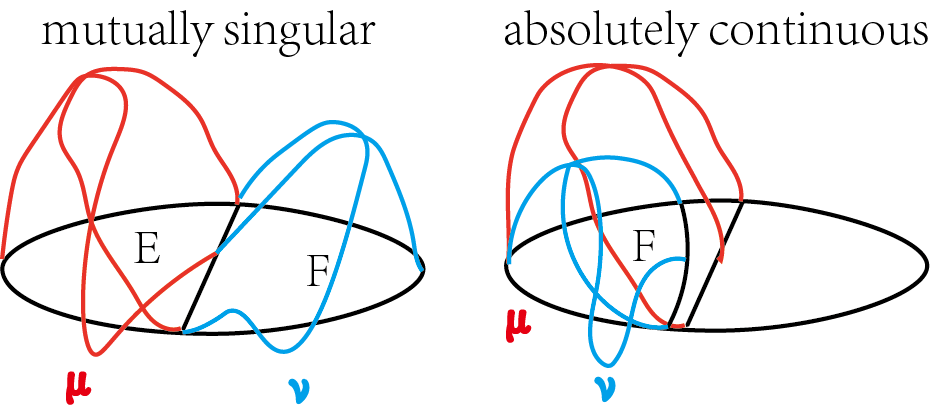
\includegraphics[width=0.5\textwidth]{ch3-pics.assets/absctn.png}
    \caption{mutually singular and absolutely continuous}
    \label{mutually singular and absolutely continuous}
\end{figure}
\textbf{$\nu \bot  \mu$ 表示的是 $\nu$ 和 $\mu$ 出现变化的区域完全不同}, 而 \textbf{$\nu \ll \mu$ 表示的是 $\nu$ 出现变化的区域完全包括在 $\mu$ 出现变化的区域里 }(因为 $\mu$ 不变化的区域被包括在 $\nu$ 不变化的区域里).
 
\begin{example}
    $f \in L^1 (\mu)$, $\nu(E) : = \int_E f \, d\mu$, 由积分定义出的 s.m., 总是满足 \[
    \nu \ll \mu
    \]
\end{example}
\begin{example}\[
    \nu_1 : = m,\quad \nu_2 := \sum_{j=1}^\infty c_j \delta_{x_j},\quad \nu_3 : = \mu_{Cantor}
    \]
    这三个 measure 有 \[
    \nu_i \not \ll \nu_j \quad \forall i\not = j
    \]
    它们是 mutually singular 的. 对于其中任意两个 $\nu_i,\nu_j$, 本身已经存在一个划分使得 $\nu_i$ 在 $E$ 上是 null 的而 $\nu_j$ 在 $E^c$ 上是 null 的. 那么如果 $\nu_i \ll \nu_j$, 则说明 $\nu_i$ 在 $E^c$ 上也是 null 的, 那么 $\nu_i$ 在整个 $X$ 上都是 null 的, 说明 $\nu_i$ 是一个 trivial measure.\\
    显然, 这里三个 measure 都不是 trivial measure, 因而它们之间没有 abs ctn 的关系.
\end{example}

\begin{proposition}{absolutely continuous 的性质}
\begin{itemize}
    \item \[ |\nu | \ll \mu \iff  \nu ^+ \ll \mu \text{ and } \nu^- \ll \mu  \](容易证明)
    \item \[  \nu \bot \mu \text{ and } \nu \ll \mu \implies \nu = 0  \](刚才已经证明)
\end{itemize}    
\end{proposition}
我们可以把 absolutely ctn 的概念从一个 s.m. wrt 一个 p.m. 扩展到一个 s.m. wrt 一个 s.m., by taking 后面这个 s.m. 的 total variation measure: \[
\text{say } \nu \ll \mu, \text{ if }  \nu \ll |\mu|
\]
但是 Folland 表示我们之后并不需要用到这个更 general 的定义. 所以不用在意它.

\subsection{$\nu \ll \mu$ 的等价条件}
We do have a question: 为什么这个定义要叫做 absolutely continuous, 它和 continuous 到底有什么关系. 下面这个 theorem 可以说明.
\begin{theorem}{why it is called "absolutely continuous"}
    令 $\nu$ 为一个 \textbf{finite s.m.}, $\mu$ 为一个 \textbf{p.m.} on $(X,\mathcal{A})$.\\
    Claim: \[\nu \ll \mu \iff \forall \, \epsilon>0,\, \exists  \, \delta > 0 \;\text{s.t.}  \;|\nu(E)| <\epsilon  \text{ whenever } \mu(E)< \delta  \]
\end{theorem}
\begin{remark}
   $\nu$ abs ctn w.r.t. $\mu$ ($\nu$ 出现变化的区域完全包括在 $\mu$ 出现变化的区域里) 等价于: 我们可以用一个集合的 $\mu$ 的大小来控制  $\nu$ 的大小 //TODO
\end{remark} 
\begin{proof}
    (i) to (ii): 我们使用反证, assume (i), 并 suppose for contradiction that (ii) 不成立.\\
    那么存在 $\epsilon > 0$ s.t. 对于任意 $n \in \mathbb{N}$, 都存在一个 seq $E_n \in \mathcal{A}$ s.t. $\mu(E_n) \leq \frac{1}{2^n}$, $\nu(E_n) \geq \epsilon$ for each $n$.\\
    Set  \[
    E :  = \limsup_n E_n  = \bigcap_{n=1}^\infty \bigcup_{k=n}^\infty E_k
    \]
    我们标记后面的每个集合为: \[
    F_n: = \bigcup_{k=n}^\infty E_k
    \]
    于是 \[
    \mu(F_n) \leq \sum_{k=n}^\infty \frac{1}{2^k} = \frac{1}{2^{n}}
    \]
    从而得到, \[
    \mu(E) = 0
    \]
    而由于 $\nu(F_n) \geq \epsilon$ for each $n$, we have \[
    \nu(E) \geq \epsilon
    \]这与 $\nu \ll \mu$ contradict.
\end{proof}


\section{Radon-Nikodym derivative and RN Thm}
\begin{definition}{Radon-Nikodym derivative}
    对于 \(\begin{cases}
        \text{p.m. } \mu\\
        \text{s.m. } \nu
    \end{cases} \) on $(X,\mathcal{A})$, 如果存在一个 function $f \in L^1(\mu)$, 使得 \[
    \nu(E) = \int_E f\, d\mu,\quad \forall E \in \mathcal{A}
    \]
    则称 \textbf{$f$ is the Radon-Nikodym Derivative of $\nu$ w.r.t. $\mu$.} 写作 \[
    f = \frac{d\nu}{d\mu}
    \]或者  \[
    d\nu = f d\mu
    \]
\end{definition}
Radon-Nikodym derivative $f$ 刻画的是\textbf{在每一点 $x\in X$ 上, signed 测度 $\nu$ 相对于测度 $\mu$ 的变化速率.}\\
\begin{example}
 取一个 $\mu_F$ 
\end{example}



Question: 我们如何判断这个 RN derivative 是否存在呢? Radon Nikodym Theorem 正是这个问题的答案. 
\begin{theorem}{Radon-Nikodym Theorem}
    对于 \(\begin{cases}
        \text{p.m. } \mu\\
        \text{s.m. } \nu
    \end{cases} \) on $(X,\mathcal{A})$, 如果 \textbf{$\nu,\mu$ 都 $\sigma$-finite}, 那么 \[
    \nu \ll \mu \iff \exists f = \frac{d\nu}{d\mu}\in L^1(\mu)
    \]
    并且这个 RN derivative \textbf{$f$ 是 \textbf{unique 的, in $\mu$-a.e. sense.} }(即在 $\mu$ 的一个 null set 之外唯一).
\end{theorem}
Radon Nikodym Theorem 表示, 对于 $\sigma$-finite 的 $\nu$ 和 $\mu$, RN derivative 存在(并且)当且仅当 $\nu \ll \mu$.\\
RN Thm 量化了 absolutely continuous 这个概念: \textbf{对于任意两个 abs ctn 的 measure, 只要它们 $\sigma $-finite, 就可以用一个具体的函数 $f$ 来表达它们之间的关系.}\\

要证明 RN Theorem, 我们还需要一些 Lemma.











下一个 lecture: 我们将 upgrade RN Thm to 一个更加 general 的 version: Lebesgue Radon Nikodym Thm.











\chapter{Lebesgue-Radon-Nikodym Theorem}
recall: Given s.m. $\mu, \nu$ on $(X,\mathcal{A})$, 我们称 $\mu$ 和 $\nu$ 是 mutually singular 的:   \[
\mu \bot \nu 
\]if $X = E \sqcup F$, $E$ 是 $\mu$ 的 null set, $F$ 是 $\nu$ 的 null set.
我们称 $\nu$ is absolutely continuous with respect to $\mu$: \[
\nu  \ll \mu 
\]
if 所有 $\mu$ 的 null set 也都是 $\nu$ 的 null set.


Jordan Decomposition Theorem: 任何 signed measure 都可以被拆分为两个 mutually singular 的 p.m. 的 difference \[
\nu = \nu^+ - \nu^-
\]

Radon-Nikodym Theorem: \[
\begin{cases}
    \mu \; \sigma\text{-finite p.m.} \\
     \nu \; \sigma\text{-finite s.m.} \\
     \nu \ll \mu
\end{cases}\implies \begin{cases}
    \exists !\; \text{extended } \mu\text{-integrable}\; f: X\to \mathbb{R}\\
    d\nu = f d\mu
\end{cases}
\]

我们称 $f$ 为 Radon-Nikodym Derivative. \[
\nu(E) = \int_E f \; d\mu
\]


\begin{example}
Application: conditional expectation.\\
\[
(X,\mathcal{A},\mu)  := \bigg([0,1), \mathcal{B}([0,1)), m\bigg)
\]
$f:[0,1) \to \mathbb{R}$ Borel measurable.\\
Define: \[
B: = \{\varnothing, [0,\frac{1}{2}), [\frac{1}{2},1),X  \}
\]
$f$ 并非一定是 $B$-measurable 的. 

\end{example}




\begin{theorem}{Lebesgue-Radon-Nikodym Theorem}
    如果 $\begin{cases}
    \mu \; \sigma\text{-finite p.m.} \\
     \nu \; \sigma\text{-finite s.m.} 
\end{cases}$ on $(X,\mathcal{A})$, 那么存在唯一的 decomposition \[
\nu = \lambda + \rho 
\]where $\lambda, \rho$ 是 $\sigma$-finite 的 signed measure s.t. $\begin{cases}
    \lambda \bot \mu \\
    \rho \ll \mu
\end{cases}$.\\
并且, 存在唯一的 extended $\mu$-integrable $f:X\to \mathbb{R}$ s.t. \[
d \rho = f \,d\mu
\]
(This is the RN part.)
\end{theorem}




\begin{lemma}
    如果 $\mu,\nu$ 是 \textbf{finite p.m.} on $(X,\mathcal{A})$, 那么它们 either $\mu\bot \nu$, or 存在 $\epsilon>0$ 和 measurable $E$ s.t. $\mu(E) > 0$ 并且 $\nu  > \epsilon \mu$ on $E$. 
\end{lemma}



\begin{lemma}
    如果 $\mu,\nu$ 是\textbf{ s.m.} on $(X,\mathcal{A})$, \[\begin{cases}
        \nu \ll \mu \\
        \nu \bot \mu
    \end{cases} \implies \nu  = 0 \]
\end{lemma}


Sktech of proof of LRN theorem: 
Assume for simplicity that $\mu,\nu$ 是 finite p.m.\\
Like last time, look at \[
\mathcal{F} : =  \{f\in L^+ : \int_E f\, d\mu \leq \nu(E) \;\; \forall E\in\mathcal{A}  \} / \sim
\]
Saw: $\mathcal{F} $ 有 max element $f$.\\
Define $\rho$ by $d \rho = f \, d \mu$.\\
Set: \[
\lambda : = \nu - \rho
\]
Want: $\lambda \bot \mu$.\\
Prove by contradiction: 如果 $\lambda \not \bot \mu$, 那么Lemma 2 告诉我们: 存在 $\epsilon > 0$ 和 positive measure 的 $E \in \mathcal{A}$ 使得: \[
\lambda \geq \epsilon \mu
\]
on $E$.\\
Set \[
g: = f + \epsilon\chi_E 
\]
则 \[
\int_F g \, d\mu = \int_{F \cap E} (f + \epsilon)\, d\mu \, + \, \int_{F \cap E^c} f \, d\mu
 \]
因而 \begin{align*}
    \rho (F \cap E)  + \epsilon \mu (F \cap E) + \rho (F \cap E^c) &= \rho(F) + \epsilon \mu(F \cap E) \\
    &\leq \nu(F) - \epsilon \mu(F)  + \epsilon \mu (F\cap E) \\
    &\leq \nu(F)
\end{align*} 
因而 $g \in \mathcal{F}$ 且 $g > f$.\\
从而得证 $\lambda \bot \mu$. 从而 existence proved.\\
Uniqueness part: Suppose we have \[
\nu = \lambda_1 + \rho_1 = \lambda_2 + \rho_2
\]
where $\lambda_i \bot \mu$, $\rho_i \ll \mu$.
那么 \[
\lambda_1  - \lambda_2 =  \rho_2 - \rho_1
\]
我们知道, $\lambda_1  - \lambda_2 $ 和 $ \rho_2 - \rho_1$ 也是 signed measures. 并且, 
\[
(\lambda_1  - \lambda_2) \bot \mu ,\quad ( \rho_2 - \rho_1) \ll \mu 
\]
By Lemma 1: \[
\lambda_1  - \lambda_2 =  \rho_2 - \rho_1 = 0
\]





Properties of the RN derivative:
(P91 in Folland)
\[
\frac{d(\nu_1 + \nu_2)}{d \mu} = \frac{d \nu_1}{d\mu} + \frac{d\nu_2}{d \mu}
\]
\[
\nu \ll \mu ,\mu \ll \mu \implies \frac{d\nu}{d\mu} \frac{d\mu}{d\nu}  = 1
\]
$\mu$-a.e. = $\nu$-a.e.













\chapter{the dual of $L^p$}
对应: Folland 5.1, 5.2, 6.2.\\
原本这是在 lec 25 的位置讲的, 但是当时由于没有 Radon-Nikodym Thm, 没有足够的工具去完成 \[
(L^p)^* = L^q
\]
的证明 (差了一个 proof surjectivity of the isometry $g \to \ell_g$). 不清楚老师为什么要把它放在这里讲. 因而我把它放在 Ch3 讲完后的位置了.\\
我们首先练习一个 example of Hölder's ineq 来回忆一下:\\
recall Hölder's ineq: for $1\leq p,q\leq\infty,\; \frac{1}{p}+\frac{1}{q} = 1\implies$ \[
||fg||_1 \leq ||f||_p ||g||_q
\]
\begin{example}
Prove:\[
    f \in L^3 ([-1,1],m)\implies \int_{-1}^1 \frac{|f(x)|}{\sqrt{|x|}} \,dx < \infty
    \]
\begin{proof}
    Apply Hölder's: 既然 $f\in L^3$, 那么我们就拉满, take $p=3$, correspondingly $ q=3/2$:\begin{align}
        \int_{-1}^1 \frac{|f(x)|}{\sqrt{|x|}} \,dx   &\leq \bigg(\int_{-1}^1 |f(x)|^3\, dx\bigg)^\frac{1}{3} \bigg(\int_{-1}^1  \frac{1}{|x|^{\frac{3}{4}}} \,dx    \bigg)^\frac{2}{3}
    \end{align} both integrals evaluate $<\infty$
\end{proof}
\end{example}

\section{intro to dual space}
这里只讨论 $\mathbb{K} := \mathbb{R}$ or $\mathbb{C}$.\\
recall, 对于一个 $\mathbb{K}$-vector space $V$, 一个 linear functional of $V$ 就是一个 linear function \[
f:V \to \mathbb{K}
\]
对于作为 NVS 的 $V$, 我们还可以定义一个 linear functional 的 boundedness. 
\begin{definition}{bounded linear functional }
 Let $V$ be a $\mathbb{K}$-NVS, $f:V \to \mathbb{K}$ be a linear functional.\\
 我们称 $f$ bounded, if exist $C>0$ s.t. \[
|f(v)| \leq C||v||,\quad \forall \,v \in V
\]
\end{definition}
\begin{remark}
注意, \textbf{linear functional 的 boundedness 和它作为函数的 boundedness 是不一样的概念.}\\
作为函数的 boundedness 表示函数值的有界性, 而\textbf{作为  linear map 的 boundedness (此处) 表示它的作用效果的 boundedness, 不会把一个 vector 放大太多倍.}
\end{remark}

\begin{proposition}{linear functional bounded $\iff$ ctn at $0$}
    if $f:V\to \mathbb{K}$ is a linear functional, TFAE:
    \begin{itemize}
        \item $f$ bounded
        \item $f$ continuous
        \item $f$ continuous at $0\in V$
    \end{itemize}
\end{proposition}
\begin{proof}
    (ii) to (iii): trivial.\\
    (i) to (ii): 假设 $f$ bounded, 那么可以 pick $C$ s.t. $|f(v)| \leq C||v||$.\\
    Pick $v_0\in V, \epsilon > 0$. Set $\delta := \frac{\epsilon}{C}$. Then
\[
    ||v-v_0|| <\delta \implies |f(v)-f(v_0)| = |f(v-v_0)| \leq C||v-v_0|| < \epsilon
    \]
   从而 ctn.\\
    (iii) to (i): $\exists \delta > 0$ s.t. $||v|| \leq \delta\implies |f(v)|\leq 1$.\\
    于是 $\forall v \in V\setminus \{0\}$, 都有 \[
    |f(v)| =   \frac{\big|f(v \cdot \frac{\delta}{||v||} ) \big| }{\frac{\delta}{||v||}}   \leq \frac{\delta}{||v||}
    \] taking $C =\frac{1}{\delta}$, 得到 boundedness.
\end{proof}
\begin{remark}
    这个 proposition 看起来很神奇, 把一个整体性质和局部性质等价了, 但是我们知道 linear map 就是局部决定整体的, by its def.\\
 recall in 395: 实际上这个性质应该对所有的 linear map 都成立, 不只是 linear functionals. \\
 通常我们认为 linear map 总是 ctn 的, 但是其实它 ctn iff bounded, unbounded 的时候就不 ctn.\\
 以及: \textbf{linear map between finite dim spaces 总是 bounded 的, 从而总是 ctn 的}. 不过这里我们要讨论的就是 infinite dim spaces. 比如 $L^p$.
\end{remark}


\begin{definition}{dual space}
If $V$ is a NVS, 我们定义它的 \textbf{dual space} as: \[
    V^* := \{\text{bounded linear functionals }\; f: V \to \mathbb{K}  \}
    \]
\end{definition}



\begin{definition}{norm of dual space: 即 \textbf{dual norm}}
    Given $f \in V^*$, set \[
    ||f||_* : = \sup_{v\in V\setminus \{0\}} \frac{|f(v)|}{||v||} = \sup_{||v||=1} |f(v)|
    \]
  where $\| v\|$ 表示的是 $V$ 上使用的 norm. 这个 norm 被称为 dual norm.
    \end{definition}
        这个形式是我们在各种地方见过非常多次的\textbf{ }operator norm, 只不过这里, 指定一个 NVS, 对于其 dual space 上的 linear functional, 它是固定的, 不需要指定 $v$ 和 $f(v)$使用哪个 norm, 因为 $f(v)$ 就是标量, 而 $v$ from 原  NVS, 已经指定好 norm. 
\begin{remark}
    从定义中我们可知, 对于任意的 $v\in V$, $f\in V^*$, 都有: \[
    |f(v)| \leq \|f \|_*|v|
    \]
\end{remark}
        
\subsection{$V^*$ being a Banach space}
\begin{theorem}{dual space is always Banach}
对于\textbf{任意的 NVS }$V$: $V^*$ 都是一个 Banach space. (not assuming $V$ Banach).
\end{theorem}
\begin{proof}
First we can confirm $V^*$ is a VS, 因为它由 linear functions of the same size 组成. \\
\textbf{Claim 1: $V^*$ 是一个 NVS.}\\
因为任取 $v\in V,\lambda\in\mathbb{K}$ 都有 $|f(\lambda v)| = |\lambda|\cdot |f(v)|$, 从而
\[
f \in V^* ,\lambda \in \mathbb{K}        \implies ||\lambda f||_* = |\lambda| \cdot ||f||_*
\]以及 \[
f,g\in V^*, v\in V \implies |(f+g) (v)| = |f(v) + g(v)|  \leq |f(v)| + |g(v)|
\]因而
\[
f,g\in V^* \implies \|f+g\|_* \leq \|f\|_* + \|g\|_*
\]
下面我们 verify $V^*$ Banach.\\
\textbf{Claim 2: 一个 Cauchy seq in $V^*$ 一定 pointwise converge to some $f 
$}\\
    Pick $(f_n)_1^\infty$, 一个 Cauchy seq in $V^*$. Let $\epsilon < 0$, 存在 $N$ 使得对于任意 $m,n \geq N$ 都有 \( \| f_n - f_m \|_* < \epsilon\), 我们简写为: \[ \|f_n - f_m\|_*  \to 0   \]
因而对于任意 $v\in V$,  we have \[
    |f_n(v) - f_m(v) | \leq \|f_n - f_m\|_*  ||v|| \to 0
    \]
并且我们知道\textbf{ $\mathbb{K}$ 是 complete 的}, 因而 $f_n(v)$ converges in $\mathbb{K}$ to some element, declared to be $f(v)$.\\
即 \textbf{\(f_n \to f \) pointwisely}:\[
    \lim _{n\to \infty} f_n (v )  = f(v)
    \]
(这是自然的, 因为如果 linear function $f-g$ 的 operator norm 是 $0$, 那么说明它们毫无差别, 否则一定有某个地方 $f,g$ 的 image 不一样, 使得这个 norm 不是 $0$.)\\
\textbf{Claim 3: $f$ 是 linear 的, 并且 bounded (从而 ctn), 即 $f\in V^*$. }\\
linearity: 由于每个 \(f_n\) 都是 linear 的, \[
      f_n(x + \alpha y) = f_n(x) + \alpha f_n(y)
      \]
因而 \[
      f(x + \alpha y) 
      = \lim_{n\to\infty} f_n(x+\alpha y) 
      = \lim_{n\to\infty}\bigl(f_n(x) + \alpha f_n(y)\bigr)
      = \lim_{n\to\infty}f_n(x) + \alpha \lim_{n\to\infty}f_n(y)
      = f(x) + \alpha f(y)\]
    因此 \(f\) 是线性的.\\
\textbf{ (Note: 这里证明了 linear map 的 pointwise 极限一定也是 linear map.)}\\
Boundedness: 
Note a standard fact from metric spaces: \textbf{every Cauchy sequence is bounded.}\\
因而 $f_n$ 是一个 bounded seq, 即存在 \(M>0\) such that \(\|f_n\| \le M\) for all \(n\). Then   \[
   |f(x)| = \big|\lim_{n\to\infty} f_n(x)\big|
            \le \lim_{n\to\infty} |f_n(x)|
            \le \lim_{n\to\infty} \|f_n\|_* \|x\|
            \le  M\,\|x\|
   \]
   Hence \(f\) is bounded (continuous), and \(\|f\|_* \le M\).
\textbf{Claim 4: $   \|f_n - f\|_*  \to 0$, proving $V^*$ 是 Banach 的.}
WTS:   \[
   \|f_n - f\| 
   = \sup_{\|x\|=1} |(f_n - f)(x) | \to 0
   \]
//TO BE DONE.
\end{proof}
Actually 这个 Theorem 有更 general 的形式: 

\begin{theorem}
对于任意 nvm $V$ 和 Banach $W$, \( \mathcal{L}(V,W)\) 一定是 Banach 的.
\end{theorem}
Proof 见 Folland 5.4.


\section{$(L^p)^* = L^q$, $\frac{1}{p} + \frac{1}{q} = 1$ }

\begin{theorem}{对于互为 conjugate exponent 的 $p,q$, $L^p$ 是 $L^q$ 的 dual space}
    
\end{theorem}

For $1 < p,q < \infty$ with $\frac{1}{p} + \frac{1}{q} = 1$, we have: \[
(L^p)^* = L^q
\]
In particular the Hilbert space: \[
(L^2)^*  = L^2
\]

\begin{proof}
    Define map \begin{align}
        L^q &\to (L^p)^* \\
        g &\mapsto \varnothing_g
    \end{align}
    where $$\varnothing_g(f) := \int fg,\quad f \in L^p $$
    It is well-defined by Hölder: \[
    f\in L^p, g\in L^q \implies fg \in L^1 
    \]
    and \[
    ||fg||_1 = \int |fg| \leq  ||f||_p ||g||_q
    \]
    Easy: \[
    \varnothing_g (f_1 + f_2) = \varnothing_g (f_1) + \varnothing_g(f_2)
    \]
    Also \[
    |\varnothing_g(f)| =\bigg|\int fg\bigg| \leq \int |fg| \leq ||f||_p\cdot  ||g||_q
    \]
    Thus \[
    \varnothing_g \in (L^p)^*\
    \]
\end{proof}







\end{document}